%\documentclass[a4paper,12pt,BCOR0mm,headsepline,draft,twoside]{scrbook}
\documentclass[a4paper,12pt,BCOR0mm,headsepline,final,oneside]{scrbook}

\usepackage{ifpdf}
\usepackage{ifdraft}

% define the type of the thesis: Studienarbeit/Diplomarbeit
% (uncomment the appropriate type)
\newcommand{\thethesis}[0]{%
  Master Thesis
}

% find all usages of \field and replace the whole expression
\newcommand{\field}[1]{%
  {\itshape \{#1\}}
}

\ifoptiondraft{%
  \usepackage[firsttwo,bottomafter]{draftcopy}
}

% include some useful packages
\usepackage{scrtime}                          % gain access to time stamps
\usepackage{scrpage2}                         % headers and footers
\usepackage{makeidx}                          % support for makeidx
\usepackage{array}                            % better table support
\newcolumntype{C}[1]{>{\centering\arraybackslash}m{#1}}
\usepackage{multicol}                         % spanning columns
\usepackage{multirow}                         % spanning rows
\usepackage{amsfonts}
\usepackage{stmaryrd} % for jump in gradient symbol
\usepackage{siunitx}
\usepackage{amsmath, bm, bbm}
\usepackage{mathtools}
\usepackage{amssymb}
\usepackage{relsize}
\usepackage{enumitem}
\usepackage[usenames, dvipsnames]{color}

\usepackage[T1]{fontenc}
\usepackage[utf8]{inputenc}
\usepackage[backend=biber,style=numeric,sorting=ynt]{biblatex}
\addbibresource{task_1_ref.bib}
\addbibresource{task_2_2_ref.bib}

\renewcommand*{\bibfont}{\small}

\usepackage[nottoc]{tocbibind}
\usepackage[final]{graphicx}
\graphicspath{{./images/}}

\usepackage{tikz,pgfplots}
\usetikzlibrary{spy}
\pgfplotsset{table/search path={./data}} %checks in data folder
\pgfplotsset{compat=newest}	%mention version to avoid warnings
\pgfplotsset{every axis/.append style={
                    label style={font=\small},
                    legend style={font=\small, draw=none, fill=none},
                    tick label style={font=\small}
                    }}
                    
\usepackage{pgfplotstable}

\DeclareMathOperator{\erf}{erf}
\DeclarePairedDelimiterX{\norm}[1]{\lVert}{\rVert}{#1}
\newcommand{\seminorm}[1]{\left\lvert #1 \right\rvert}

\usepackage{breqn}
\usepackage{empheq}
\usepackage[most]{tcolorbox}

{
%\makeatletter
% \renewcommand*\l@subsubsection{\@dottedtocline{5}{1cm}{1cm}}
%\makeatother
% section numbering depth
%\setcounter{secnumdepth}{5} % seting level of numbering (default for "report" is 3). With ''-1'' you have non number also for chapters
%\setcounter{tocdepth}{5} % if you want all the levels in your table of contents
}
% include right printer driver for graphicx
%\ifpdf
%  \usepackage[pdftex]{graphicx}
%  \pdfcompresslevel=9
%\else
%  \usepackage[dvips]{graphicx}
%\fi

\usepackage{caption}
\usepackage{subcaption}
%\usepackage[export]{adjustbox}

\usepackage[ngerman,english]{babel}           % switch language
\usepackage{float}                           
\usepackage{nomencl}                          % list of abbreviations
\usepackage[ruled,vlined,algochapter]{algorithm2e}
%\usepackage{algorithmic}                      % typesetting of algorithms
%\usepackage[ruled,chapter]{algorithm}         % typesetting of algorithms
\usepackage{stfloats}                         % used to have footnotes at bottom of the page
%\usepackage[final]{listings}                  % typesetting of code listings 
\usepackage{hyperref}
\usepackage[capitalise, noabbrev]{cleveref}
\usepackage{xcolor}
\hypersetup{
  colorlinks   = true, %Colours links instead of ugly boxes
  urlcolor     = red, %Colour for external hyperlinks
  linkcolor    = blue, %Colour of internal links
  citecolor    = red,  %Colour of citations
  menucolor    = red
}



% define command \missing
\newcommand{\missing}[1]{\,\,(\marginpar[\hfill!$\longrightarrow$]{$\longleftarrow$!}{\bfseries 
    Missing:}\,\emph{#1})\,\,}
\newcommand{\note}[1]{\marginpar[#1]{#1}}
\newcommand{\code}[1]{\texttt{#1}}

% environment to typeset sub-figures
\newbox\subfigbox
\makeatletter
        \newenvironment{subfloat}
                {\def\caption##1{\gdef\subcapsave{\relax##1}}%
                 \let\subcapsave\@empty
                 \setbox\subfigbox\hbox
                         \bgroup}
                  {\egroup
                 \subfigure[\subcapsave]{\box\subfigbox}}
\makeatother

% list of abbreviations
\let\abbrev\nomenclature
\renewcommand{\nomname}{List of Acronyms}
\setlength{\nomlabelwidth}{.25\hsize}
\renewcommand{\nomlabel}[1]{#1 \dotfill}
\setlength{\nomitemsep}{-\parsep}
\makeglossary
\newcommand{\markup}[1]{\textbf{#1}}

% define new style for TOC
\makeatletter
\renewcommand{\numberline}[1]{%
        \makebox[0.9cm][l]{#1}\hspace{1mm}}
\renewcommand{\l@chapter}[2]{%
        \addvspace{2ex}%
        \pagebreak[3]%
        \noindent%
        \makebox[0pt][l]{%
        \rule[-3pt]{\textwidth}{0pt}}%
        {\large\textsf{\textbf{#1}}}\hfill#2%
        \par%
        \nopagebreak%
        \addvspace{1ex}%
}
\renewcommand{\l@section}[2]{%
        \addvspace{0.5ex}%
        \noindent\hspace{1cm}%
        #1\dotfill#2%
        \par%
        \nopagebreak[2]%
}
\renewcommand{\l@subsection}[2]{%
        \addvspace{0.2ex}%
        \noindent\hspace{2cm}%
        #1\dotfill#2%
        \par%
}       
\makeatother

% define new style for index 
\makeatletter
\newcommand*{\heading}[1]{%
        \makebox[0pt][l]{%
                \rule[-3pt]{\linewidth}{0pt}}%
        \textsf{\textbf{\Large #1}}\hfill\nopagebreak\vspace{4pt}}
\renewenvironment{theindex}{%
        \setlength{\columnseprule}{0.4pt}
        \setlength{\columnsep}{2em}
        \begin{multicols}{2}[\chapter*{\indexname}]
                \parindent\z@
                \parskip\z@ \@plus .3\p@\relax
                \let\item\@idxitem}%
        {\end{multicols}\clearpage}
\makeatother

% page break
\clubpenalty = 10000
\widowpenalty = 10000

% prepare generation of index
\makeindex

% put footnotes below floats at the bottom
\fnbelowfloat

\begin{document}

\frontmatter
\begin{titlepage}

  \begin{center}
    
    {\LARGE \bf
      \textbf{MODELLING OF INSTABILITIES IN MAGNETO-ELASTIC MEMBRANES}\\
    } 
    
    \vspace*{1.5cm}
    {\Large{\textbf{\thethesis} \\in the study programme Computational Engineering}}
    \vspace{1.5cm}
    
    {\large submitted by} \\
    \vspace*{0.5cm}
    {\Large \bf \text{Vinayak Balasaheb Gholap}} \\
    \vspace*{0.2cm}
    {\large \bf \text{Matriculation number: 22065422}} \\
    \vspace*{0.2cm}
    {\large born on \text{01.11.1993} in \text{Pune, India}} 
    
    \vspace{1.5cm}
    
    {\large performed at}

    \vspace{0.5cm}
    
    {\bf 
      %Department  \\
      Lehrstuhl f\"ur Technische Mechanik\\
      Friedrich-Alexander-Universit\"at Erlangen--N\"urnberg \\
      (Prof. Dr.-Ing. habil. Paul Steinmann)
      }
    
    \vspace{1cm}
    \begin{tabular}{rl}
    \textbf{Examiner:}& Prof. Dr.-Ing. habil. Paul Steinmann \vspace{0.5cm} \\    
    \textbf{Supervisors:}& Dr. Jean-Paul Pelteret (FAU Erlangen, Germany)\\
    		 & Dr. Prashant Saxena (University of Glasgow, UK) \vspace{0.5cm} \\    
   % Beginn der Arbeit: \field{Date} \\
    \textbf{Date of submission:}& \today
    \end{tabular}
    
  \end{center}
  
\includegraphics[width=4cm]{ltm.png}\hspace*{4cm}~
\includegraphics[width=7.5cm]{logo_fau.jpg}
\end{titlepage}

\clearpage{\pagestyle{empty}\cleardoublepage}

\thispagestyle{empty}
\selectlanguage{ngerman}
Ich versichere, dass ich die Arbeit ohne fremde Hilfe und ohne Benutzung
anderer als der angegebenen Quellen angefertigt habe und dass die Arbeit in
gleicher oder \"ahnlicher Form noch keiner anderen Pr\"ufungsbeh\"orde
vorgelegen hat und von dieser als Teil einer Pr\"ufungsleistung angenommen
wurde. Alle Ausf\"uhrungen, die w\"ortlich oder sinngem\"a\ss{} \"ubernommen
wurden, sind als solche gekennzeichnet.

\vspace{2cm}

Der Universit\"at Erlangen-N\"urnberg, vertreten durch die Lehrstuhl f\"ur Technische Mechanik, wird f\"ur Zwecke der Forschung und Lehre ein einfaches,
kostenloses, zeitlich und \"ortlich unbeschr\"anktes Nutzungsrecht an den
Arbeitsergebnissen der \thethesis einschlie\ss{}lich etwaiger Schutzrechte und
Urheberrechte einger\"aumt.

\vspace{2cm}
Erlangen, den \today

\vspace{2cm}
\text{Vinayak Gholap} \hfill \ 

\vspace{0,5cm}

\clearpage{\pagestyle{empty}\cleardoublepage}
\pagenumbering{roman}

\selectlanguage{english}
{
\pagestyle{empty}
\begin{center}
\Huge \bf Tasks
\end{center}

\begin{enumerate}
\item[Task 1] Magneto-static magnetic scalar potential (MSP) formulation:
\begin{enumerate}
\item Literature survey on non-linear magneto-elasticity and its finite element modelling \cite{dorfmann2004, dorfmann2005, reddy_toroid, barham}
\item Devise a method of modelling the thin tubular membrane toroidal geometry using the MSP formulation 
\item Set up simulation code for the 3D and axisymmetric (2.5D) problem
\item Validate the axisymmetric formulation 
\end{enumerate}
\item[Task 2] Quasi-static finite strain elasticity problem:
\begin{enumerate}
\item Understand and implement a quasi-static finite-strain elasticity problem for pure mechanical loads and deformations \cite{Pelteret2016a, Pelteret2012}
\item Extend the application code from Task 1 for the axisymmetric formulation of the MSP problem to a coupled magneto-elastic problem known as a vector-valued problem
\item Implement a constitutive material law considering the geometric and material non-linearity of an isotropic continuum elastic body \cite{Wriggers2008}
\item Implement an iterative Newton method with (quasi-static linear) load incrementing algorithm to solve the non-linear system of equations for the vector-valued displacement solution
\item Test the developed code with mechanical test problems that exhibit finite deformations with instability/buckling characteristics
\end{enumerate}
\item[Task 3] Coupled magneto-elasticity problem:
\begin{enumerate}
\item Implement a material model for the coupled problem \cite{pelteret2016, Saxena2015}
\item Extend the application code incorporating the conclusions drawn from Task 1 and Task 2
\item Implement a segregated iterative solver from the literature \cite{Benzi2005} to solve the coupled saddle point system
\item Examine material behaviour at high mechanical and magnetic loads for material instability
\end{enumerate}
\item[Task 4] Path-following solution methods:
\begin{enumerate}
\item Literature survey of the path-following non-linear solvers \cite{Vasios, Wriggers2008, Riks1979, CRISFIELD1981}
\item Implement the Arc-Length solver considering the Crisfield method
\end{enumerate}
\end{enumerate}
\pagestyle{scrheadings}
}
\pagenumbering{roman}
\pagestyle{empty}
\chapter*{Acknowledgments}
\indent This report is the official document of the Master Thesis conducted for 30 ECTS by Vinayak Gholap in the course of M.Sc. Computational Engineering. \par
I would like to specially thank my advisor Dr.\,Jean-Paul Pelteret for providing me this interesting topic and for his continuous support, guidance and honest remarks during the course of this work. He has given me the freedom and time to work on my concepts and help me channelize our ideas into appropriate direction. I also thank my second supervisor Dr.\,Prashant Saxena for his valuable feedbacks on the documentation and his insightful suggestions to overcome the hurdles and difficulties that we faced in the course of this research. This project would have not been possible without the many fruitful discussions and conversations the three of us have had. \par  
I would like to thank Prof.\,Dr.-Ing.\,Paul Steinmann for providing the working environment at his chair. His insightful courses have been instrumental in my personal knowledge development over the past three years. \par 
I would like to sincerely express my gratitude to all the people who have helped me continuously through this exciting journey. A cheerful shout-out to Dr.\,Denis Davydov for introducing me to the \texttt{deal.II} library through a project opportunity which helped me with an easy start to my thesis. I would specially like to thank the \texttt{deal.II} community group and the contributors for the wonderful platform they have build to share and communicate the thoughts with other people. \par 
Above all, I would like to express my sincere gratitude to my family and my brother and sisters in India and my friends in Germany for their kind love and persistent belief in me throughout my studies. The moral support and love that I received from them has made this journey comfortable and worthwhile. \newline\par 

\noindent Vinayak Gholap \par 
\noindent Erlangen, \today

\clearpage{\pagestyle{plain}\cleardoublepage}


\chapter*{Abstract}
 
\clearpage{\pagestyle{plain}\cleardoublepage}

\tableofcontents
\listoffigures
\listoftables
\listofalgorithms

\mainmatter
\pagestyle{scrheadings}
\chapter{Introduction}
\label{chap:1}

\section{Motivation}
Magnetorheological elastomers (MREs) are soft materials which consist of micron sized iron particles dispersed in an elastomeric matrix. Magneto-active polymers (MAPs) termed as smart materials of future are capable to change their mechanical properties under the application of magnetic loads. This is due to the interaction of the ferrous magnetizable particles which gives rise to a coupled magneto-mechanical effect. In the presence of an external magnetic field, the magnetization vectors in iron particles align with the externally applied magnetic field and this causes a change in the mechanical stiffness and the macroscopic deformation of the polymer. Various polymers such as natural and synthetic rubber, hydrogels, silicon elastomers and polyurethanes have been utilized as the matrix material to synthesize MAPs \cite{Hana}. The different magnetic filler particles used are iron particles in micro- and nano-size. The proportion of these filler particles is usually between 0 and 30\% by volume of the entire mixture \cite{Saxena2015}. The finite deformations arising from the coupled interaction of the magnetic and mechanical fields is desired in many industrial applications. MAPs are synthesized and tuned with different micro-structural properties for a variety of applications such as magnetic actuators and vibrational dampers in mechatronic sensors and artificial muscles in the biomedical field. \par 
Motivated by the plethora of applications, the theory of MAPs macroscopic behaviour at continuum level proposed by \cite{tiersten1964coupled, brown1966magnetoelastic} is reviewed again by researchers. New modelling approaches were recently developed by \cite{kovetz2000electromagnetic, KANKANALA, dorfmann2004, dorfmann2005, ogden2011mechanics, Dorfmann2014}. These recent contributions form the theoretical foundation for the present work described in this thesis. In the work by \cite{dorfmann2004, dorfmann2005} it was pointed out that any one of the three magnetic vector fields, namely the magnetic field $\mathbb{H}$, the magnetic induction $\mathbb{B}$ and the magnetization $\mathbb{M}$, can be used as an independent input field to proceed with the mathematical modelling. The other two fields can be obtained through constitutive relations. Two different formulations depending on the choice of the independent field, termed as the scalar magnetic potential formulation and the vector magnetic potential formulation, were presented in \cite{dorfmann2004, dorfmann2005}. The difficulties arising in terms of numerical modelling and the restrictions on the choice of the class of constitutive material models to describe MAPs was also highlighted therein. \par
The solution of non-trivial boundary value problems through numerical modelling was the obvious next step in understanding the nature of the coupled response of these smart materials. The elastic partial differential equations (PDEs) for the material deformation and the magnetic PDEs for the magnetic field are solved using the favourable discretization approach such as Finite Element method (FEM). FE simulations of the deformations of the magneto-elastic materials have been performed considering different geometries of interest in \cite{barham, bustamante2011numerical, Vogel2014}. Due to the applications of MAPs in the critical fields such as aerospace and biomedical engineering, the investigation of the failure and stability analysis of the materials under applied loads is of vital importance. Research studies in understanding the material behaviour near critical limit points and post limit points is carried out both analytically and numerically considering an isotropic and anisotropic material micro-structure in \cite{rudykh2013stability, reddy_toroid, Reddy2018, Barham2008, Miehe2015}. In an isotropic MRE, the iron particles are distributed randomly in the matrix and the resulting macroscopic response is thus isotropic. In an anisotropic MRE, the particles are arranged in chains due to the curing process during the fabrication of the material. Different numerical experiments were carried in this direction considering the chain-like micro-structure \cite{Saxena2015} and a multiscale approach using computational homogenization in \cite{keip2016multiscale}. \par 
Of particular interest to this thesis are the recent studies carried out in \cite{reddy_toroid, Reddy2018} for isotropic MREs with axisymmetric geometries under inflating pressure loads. In case of membranes of finite thickness it is already known from the stability and buckling analysis that the elastic limit points are an important phenomenon during the free inflation of these thin membranes under finite pressure loads. At the critical limit points, the membranes start to deform significantly under a slight increase of pressure load. The material softens and due to reduced stiffness we may observe buckling or wrinkling effects in the membranes. The behaviour of the material beyond these limit points leads to multiple equilibrium states, stable or unstable or both. Hence, it is important to know a priori the limit point and the limit pressure load a membrane can withstand before a structural failure is observed. The instability behaviour of such membranes is also dependent on the constitutive material model employed to describe the magneto-elastic material response. The presence of a magnetic limit point instability, a state where both the stable and unstable equilibriums merge and cease to exist, was described in \cite{Barham2008, reddy_toroid}. \par 
In the macroscopic modelling approaches \cite{bustamante2013, pelteret2016}, the energy contributions arising from the surrounding free space around the magneto-elastic membrane are also taken into consideration. The forces arising from the Maxwell stress developed in the free space by the permeating magnetic field are significant and thus need to be taken into account. The approach of a FE mesh with truncated free space from \cite{pelteret2016} was adopted in this thesis. The magneto-elastic membrane geometry along with the truncated surrounding free space was discretized using finite element basis in order to capture a more accurate response of the deformable membrane and the free space. The free space was modelled as an elastic deformable solid with relatively low elastic stiffness compared to the magneto-elastic membrane stiffness. \par 
The research plan for this thesis is to make an attempt to model the instabilities in the finite thickness torus membranes employing the h-adaptive mesh refinement finite elements. The lack of research in the numerical modelling of axisymmetric magneto-elastic solids modelled with the surrounding free space employing FEM is the main motivation for the thesis. Development of a robust and computationally efficient multi-physics, fully coupled finite element framework for the magneto-elasticity problems employing open-source, high-performance C++ FEM library such as \texttt{deal.II} \cite{BangerthHartmannKanschat2007, dealII90} is the basic goal. The developed framework tested with various sample models and unit tests to proof-check the correct functioning may be useful as a starting point for the further research. \par

\section{Research objectives}
The research direction and the discrete objectives aimed to achieve in this thesis are precisely listed below.
\begin{itemize}
\item Magneto-static magnetic scalar potential (MSP) formulation:
\begin{enumerate}
\item Devise a method of modelling the thin tubular membrane toroidal geometry using the MSP formulation 
\item Set up simulation code for the 3D and axisymmetric (2.5D) problem
\item Validate the axisymmetric formulation 
\end{enumerate}
\item Quasi-static finite strain elasticity problem:
\begin{enumerate}
\item Understand and implement a quasi-static finite-strain elasticity problem for pure mechanical loads and deformations \cite{Pelteret2016a, Pelteret2012}
\item Extend the application code from previous task to include finite elasticity
\item Implement a constitutive material law considering the geometric and material non-linearity of an isotropic continuum elastic body \cite{Wriggers2008}
\item Implement an iterative Newton method with (quasi-static linear) load incrementing algorithm to solve for the vector-valued displacements
\item Test the developed code with mechanical test problems that exhibit finite deformations with instability/buckling characteristics
\end{enumerate}
\item Coupled magneto-elasticity problem:
\begin{enumerate}
\item Implement a material model for the coupled problem \cite{pelteret2016, Saxena2015}
\item Extend the application code incorporating the conclusions drawn from both of the previous decoupled problems
\item Implement a segregated iterative solver from the literature \cite{Benzi2005} to solve the coupled saddle point system
\item Examine material behaviour at high mechanical and magnetic loads for material instability
\end{enumerate}
\end{itemize}

\section{Outline of the thesis}
This thesis is organised into four chapters. The first chapter introduced the magneto-active polymers and presents a short summary of the research performed and undergoing in these smart materials. It motivates the need to model the unstable behaviour of inflating membranes of finite thickness and also points to its importance in practical applications in different industries. As mentioned briefly above in the research objectives, the thesis was carried out in three major milestones described in the next three chapters. In the second chapter, the theory for non-linear magneto-elasticity is laid out. A particular axisymmetric (2.5D) and a 3D geometry for the membrane and the free space is developed. Different experiments are performed to model a magnetic field closely fitting to the desired results from the existing literature. Validation of the axisymmetric formulation is carried out by comparing the results against the results of a 3D model simulation. The third chapter is dedicated to the finite deformations of the membrane along with the free space under quasi-static inflating pressure loads. Here, the membrane is modelled employing a standard Neo-Hookean constitutive material law and the surrounding free space as another non-linear complaint elastic solid. The considered solution field is the vector-valued displacement field only. Linearisation of the non-linear quantities is carried out and a non-linear Newton solver is implemented. A number of mechanical test problems are presented to proof-check the implementation at various stages of code development and to validate the behaviour of the modelling approach. Test models are also developed from the literature to study the instability behaviour under finite strain elasticity framework and to demonstrate the failure of Newton method at/near critical limit points. The fourth chapter deals with coupling of the problems from Chapter 2 and Chapter 3. Different conclusions drawn from the results of previous chapters are taken into consideration to modify the approach in order to model the instabilities. The implemented material model in Chapter 3 is extended to account for the additional energy contribution from the magnetic loads and the coupled interaction of the elastic and magnetic fields. Corresponding linearisations for the updated material model are derived and implemented to form a linear system of equations. The solution strategies of the resulting saddle point system are discussed in detail. A test model for the coupled problem to gain understanding of the behaviour of the material under combined loads is simulated. Finally, an attempt is made to initiate and model the buckling instability in the membrane near the limit points.
\chapter{Magneto-static magnetic scalar potential}

\section{Kinematics}
We consider a magneto-elastic solid body $\mathcal{B}_0$ in a three-dimensional Euclidean space that is initially in stress-free configuration, not subjected to any mechanical or magnetic field loads. On application of a magnetic load defined by a magnetic field $\mathbb{H}$ and an associated magnetic induction $\mathbb{B}$ and magnetization vector $\mathbb{M}$, in the absence of any mechanical load, the body will undergo some deformation due to this magnetic load. This phenomenon is referred to as \textit{magnetostriction}. Let the resulting deformed configuration from the magnetostriction be denoted as $\mathcal{B}_t$. This configuration will depend on the choice of the initial magnetic field $\mathbb{H}$. \par 
Let any point in the reference configuration $\mathcal{B}_0$ be identified by the position vector $\mathbf{X}$ and it's position in the deformed configuration $\mathcal{B}_t$ be given as $\mathbf{x} = \bm{\varphi} (\mathbf{X})$. The field $\bm{\varphi}$ is a one-to-one mapping describing the deformation of the body. The associated deformation gradient $\mathbf{F}$ relative to $\mathcal{B}_0$ is defined as $\mathbf{F} := \nabla_0 \bm{\varphi}$ and it's determinant is $J = \text{det}\mathbf{F} > 0$ (non-negative to avoid material self-penetration). The gradient w.r.t. the reference configuration $\mathcal{B}_0$ is denoted as $\nabla_0$ and the gradient w.r.t. the deformed configuration $\mathcal{B}_t$ be denoted as $\nabla$. The magnetic vector fields in the deformed configuration are denoted as $\mathbbm{b}, \mathbbm{h}$ and $\mathbbm{m}$.\par 

\begin{figure}[h]
\centering 
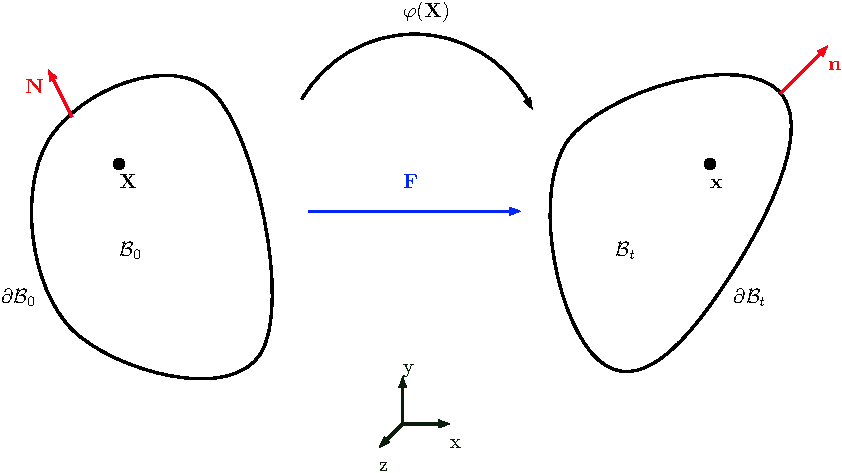
\includegraphics[width=0.65\textwidth]{kinematics_potato.pdf}
\caption{Kinematics}
\label{fig:1.1}
\end{figure} 

\section{Balance equations}
\subsection{Magnetic balance laws}
In the absence of any deformation ($\mathbf{F} = \mathbf{I}$), the magnetic quantities $\mathbbm{b}, \mathbbm{h}, \mathbbm{m}$ are related by the standard formula
\begin{equation}
\mathbbm{b} = \mu_0 (\mathbbm{h} + \mathbbm{m}),
\label{eq:1.1}
\end{equation}
where $\mu_0 = 4\pi \times 10^{-7} \text{Hm}^{-1}$ is the magnetic permeability in vacuum. \par 
For the case of time-independent problems and in the absence of external currents, from the Ampere's law we have \cite{KANKANALA} 
\begin{equation}
\text{curl} (\mathbbm{h}) = \nabla \times (\mathbbm{h}) = \mathbf{0}.
\label{eq:1.2}
\end{equation}
For the case of magneto-statics (absence of time varying electromagnetic fields), from the assumption of the absence of magnetic monopoles we have \cite{KANKANALA}\begin{equation}
\text{div}(\mathbbm{b}) = \nabla \cdot \mathbbm{b} = 0.
\label{eq:1.3}
\end{equation}
Both the Equations \eqref{eq:1.2} and \eqref{eq:1.3} are the specializations of Maxwell's equations. Equation \eqref{eq:1.1} defines the third vector field when one field is used as an independent variable and the other field is provided by an appropriate constitutive law. 

\subsection{Mechanical balance laws}
The balance law for mass conservation is given as 
\begin{equation}
\frac{d\rho}{dt} + \nabla \cdot [\rho \mathbf{\dot{x}}] = 0,
\end{equation}
where $\rho$ is the mass density in $\mathcal{B}_t$. \par 
From the balance law for linear momentum assuming that the inertial effects are negligible, we have the equilibrium equation 
\begin{equation}
\text{div} \bm{\sigma} + \bm{b}_t = \mathbf{0} \ \ \text{in} \ \mathcal{B}_t,
\end{equation}
where $\bm{\sigma}$ is the Cauchy stress tensor and $\bm{b}_t$ is the body load per unit current volume. The balance of angular momentum leads to the requirement that $\bm{\sigma}$ is symmetric. 

\section{Boundary conditions}
In order to formulate a boundary-value problem we need constitutive laws in which $\bm{\sigma}$ and $\mathbbm{b}$ are given in terms of the variables $\mathbf{F}$ and $\mathbbm{h}$. Additionally, appropriate boundary conditions must be satisfied by the fields $\mathbbm{b}, \bm{\sigma}$ and $\bm{\varphi}$. At a bounding surface of the material body in the deformed configuration, the vector fields $\mathbbm{b}$ and $\mathbbm{h}$ satisfy the standard jump conditions
\begin{equation}
\mathbf{n} \cdot \llbracket \mathbbm{b} \rrbracket = 0, \ \ \mathbf{n} \times \llbracket \mathbbm{h} \rrbracket = \mathbf{0} \ \ \text{on} \ \partial\mathcal{B}_t,
\label{eq:1.4}
\end{equation}
where the square brackets indicate a jump across the surface and $\mathbf{n}$ is the outward pointing unit normal vector to the surface in the deformed configuration $\mathcal{B}_t$. These boundary conditions enforce that the tangential component of the magnetic field, as well as the normal component of the magnetic induction, remain continuous on the boundary \cite{pelteret2016}.

\section{Magnetic scalar potential (MSP) formulation}
The magnetic field quantities ($\mathbbm{b}, \mathbbm{h}, \mathbbm{m}$) are all discontinuous over boundaries and material interfaces: $b_{1t} \neq b_{2t}, h_{1n} \neq h_{2n}$ when $\mu_1 \neq \mu_2$ (where $t$ and $n$ denote the tangential and normal components, respectively). These discontinuities are difficult to model using the finite element method simulations. Thus, a fictitious quantity such as the magnetic scalar potential $\phi$ is used in solving the magneto-elastic problems using FEM. The magnetic scalar potential formulations can be used only in the case where there are no free currents in the domain. We define a scalar potential related to the curl-free magnetic field by \cite{pelteret2016}
\begin{equation}
\mathbbm{h} := -\nabla \phi \ \ \text{in} \ \mathcal{B}_t. 
\label{eq:1.5}
\end{equation}
The continuity condition associated with $\phi$ is 
\begin{equation}
\llbracket \phi \rrbracket = 0 \ \ \text{on} \ \partial\mathcal{B}_t.
\end{equation}
The magnetic induction vector $\mathbbm{b}$ is modelled in terms of magnetic field $\mathbbm{h}$, taking $\mathbbm{h}$ as the independent field
\begin{equation}
\mathbbm{b} = \mathbbm{b}(\mathbbm{h}).
\end{equation}
We consider the magnetization ($\mathbbm{m}$) and the magnetic field $(\mathbbm{h})$ are aligned. For a material with relative permeability $\mu_r$ we have
\begin{equation}
\mathbbm{h} + \mathbbm{m} = \mathbbm{h} + (\mu_r - 1)\mathbbm{h} = \mu_r \mathbbm{h}.
\end{equation}
The relation for the magnetic induction in terms of the magnetic field using the above relation is
\begin{equation}
\mathbbm{b} = \mu_0 \mu_r \mathbbm{h}.
\label{eq:1.7}
\end{equation}

\section{Variational formulation}
In this section, we will derive the axisymmetric weak form of the magnetic balance law:
\begin{equation}
 \text{div}\mathbbm{b} = 0,
 \end{equation} 
with the body symmetric about the Y-axis in the cylindrical co-ordinate system. The boundary condition is
\begin{align}
\mathbf{n} \cdot \llbracket \mathbbm{b} \rrbracket = 0 \ \ \text{on} \ \partial\mathcal{B}_t \ (\text{Natural boundary condition}).
\label{eq:1.10}
\end{align}
Taking integration of the strong form over the whole domain we have 
\begin{equation}
\int\limits_{z} \int\limits_{y} \int\limits_{x} \nabla \cdot \mathbbm{b} \ \mathrm{d}z \ \mathrm{d}y \ \mathrm{d}x = 0 \ \ \text{in} \ \mathcal{B}_t. 
\end{equation}
The rules for co-ordinate transformation between Cartesian and Cylindrical co-ordinate system are:
\begin{align}
x &= r \cos \theta, \ y = r \sin \theta, \ z = z, \nonumber\\
\mathrm{d}x &= \mathrm{d}r, \ \mathrm{d}y = r \mathrm{d}\theta, \ \mathrm{d}z = \mathrm{d}z, \nonumber\\
\text{with} \ r &= \sqrt{x^2 + y^2} \ \text{and} \ \tan \theta = \frac{y}{x}.
\end{align}
Applying the rules for co-ordinate transformation, we have:
\begin{equation}
\int\limits_{z} \int\limits_{\theta} \int\limits_{r} \nabla \cdot \mathbbm{b} \ \mathrm{d}z \ r \ \mathrm{d}\theta \ \mathrm{d}r = 0 \ \ \text{in} \ \mathcal{B}_t.
\end{equation}
For a magnetic field (induction) invariant w.r.t. the $\theta$ co-ordinate, i.e. symmetric field about the Y-axis, we have:
\begin{align}
\int\limits_{\theta} \mathrm{d}\theta = 2 \pi \implies \int\limits_{z} \int\limits_{r} \nabla \cdot \mathbbm{b} \ \mathrm{d}z \ 2 \pi r \ \mathrm{d}r = 0 \ \ \text{in} \ \mathcal{B}_t.
\label{eq:1.6}
\end{align}
Employing the relation given by Equation \eqref{eq:1.7} we have
\begin{equation}
\int\limits_{z} \int\limits_{r} \mu_0 \mu_r \ 2 \pi r \ \nabla \cdot \mathbbm{h} \ \mathrm{d}z \ \mathrm{d}r = 0 \ \ \text{in} \ \mathcal{B}_t.
\label{eq:1.8}
\end{equation}
Equation \eqref{eq:1.8} represents the axisymmetric formulation for the considered strong form \eqref{eq:1.3} in the Cartesian co-ordinate system. \par 

\section{Finite element approximation}
For modelling using the finite element method, as stated earlier, we use the magnetic scalar potential formulation. Using the definition for the magnetic field in terms of the virtual scalar potential as given in Equation \eqref{eq:1.5}, we have
\begin{equation}
-\int\limits_{z} \int\limits_{r} \mu_0 \mu_r \ 2 \pi r \ \nabla \cdot \nabla \phi \ \mathrm{d}z \ \mathrm{d}r = 0 \ \ \text{in} \ \mathcal{B}_t.
\label{eq:1.9}
\end{equation}
We now introduce a test function $\eta$, which is an element of the function space $V$ of test functions. The unknown function $\phi$ is an element of the function space $S$:
\begin{equation}
\phi \in S \ \text{and} \ \eta \in V.
\end{equation}
Multiplying Equation \eqref{eq:1.9} with the test function $\eta$:
\begin{equation}
\int\limits_{z} \int\limits_{r} \mu_0 \mu_r \ 2 \pi r \ [(\nabla \cdot \nabla \phi)] \eta \ \mathrm{d}z \ \mathrm{d}r = 0 \ \ \forall \eta \in V.
\end{equation}
We observe different continuity requirements hold concerning the solution function $\phi$ and the test function $\eta$; $\phi$ is required to have second derivatives thus indicating continuous first derivatives, whereas there is no derivative on $\eta$. Thus the two function spaces $S$ and $V$ are not the same. This leads to an unsymmetrical formulation. To avoid this, we reformulate the above equation using integration by parts to have a symmetric formulation:
\begin{equation}
\int\limits_{z} \int\limits_{r} \mu_0 \mu_r \ 2 \pi r \ [ \nabla \cdot (\nabla\phi \ \eta) - (\nabla \phi \cdot \nabla \eta) ] \ \mathrm{d}z \ \mathrm{d}r = 0 \ \ \forall \eta \in V.
\end{equation}
Applying the Gauss divergence theorem on the first term we have:
\begin{equation}
\int\limits_{\partial \Omega} \mu_0 \mu_r \ 2 \pi r \ \nabla \phi \cdot \mathbf{n} \ \eta \ \mathrm{d}\sigma - \int\limits_{z} \int\limits_{r} \mu_0 \mu_r \ 2 \pi r \ (\nabla \phi \cdot \nabla \eta) \ \mathrm{d}z \ \mathrm{d}r = 0 \ \ \forall \eta \in V,
\end{equation}
where $\mathbf{n}$ is the outward pointing unit normal vector to the surface. Since the test function $\eta$ have to vanish on the part of boundary prescribed by Dirichlet boundary condition and considering the natural boundary condition \eqref{eq:1.10} on the rest boundary, we get the symmetric weak form
\begin{equation}
\int\limits_{z} \int\limits_{r} \mu_0 \mu_r \ 2 \pi r \ (\nabla \phi \cdot \nabla \eta) \ \mathrm{d}z \ \mathrm{d}r = 0 \ \ \forall \eta \in V.
\label{eq:1.11}
\end{equation}
We now look at the discretization of the above axisymmetric weak formulation by finite element approximation. The function spaces $S$ and $V$ belong to the Sobolev space given as
\begin{equation}
H^1 = \left\lbrace \phi : \Omega \mapsto \mathbb{R} \,\middle\vert\, \int\limits_{\Omega} \seminorm{\phi}^2 + \seminorm{\nabla \phi}^2 \mathrm{d}\mathbf{x} < \infty \right\rbrace.
\end{equation}
Let the solution space be
\begin{equation}
S = \{ \phi \in H^1, \phi|_{\partial \Omega_{D}} = \overline{\phi} \},
\end{equation}
and the test functions space be
\begin{equation}
V = \{ \eta \in H^1, \eta|_{\partial \Omega_{D}} = 0\}.
\end{equation}
The approximation of $\phi$ and $\eta$ through linear combinations of $M$ shape functions $N_i (\mathbf{x})$ with $i =1,...,M$ is given as
\begin{align}
\phi \approx \phi^h \ \text{and} \ \nabla \phi \approx \nabla \phi^h, \nonumber\\
\eta \approx \eta^h \ \text{and} \ \nabla \eta \approx \nabla \eta^h.
\end{align}
The approximate solutions $\phi^h$ and test functions $\eta^h$ have to be chosen from the discrete function spaces 
\begin{align}
S^h &= \left\{\phi^h \in S : \phi^h(\textbf{x}) = \sum_{i=1}^{\textit{M}} \phi_i N_i (\textbf{x}), \ \phi_i \in \mathbb{R} \right\} \ \text{and} \nonumber\\
V^h &= \left\{\eta^h \in V : \eta^h(\textbf{x}) = \sum_{j=1}^{\textit{M}} \eta_j N_j (\textbf{x}), \ \eta_j \in \mathbb{R} \right\}.
\end{align}
The shape functions $N_i (\mathbf{x})$ are chosen such that the approximations $\phi^h$ and $\eta^h$ follow the continuity requirements and the prescribed boundary conditions. Inserting the approximations in Equation \eqref{eq:1.11}, we have
\begin{equation}
\int\limits_{z} \int\limits_{r} \sum\limits_{i=1}^{M} \sum\limits_{j=1}^{M} \mu_0 \mu_r \ 2 \pi r \ \phi_i \ \eta_j \Big( \nabla N_i (\mathbf{x}) \cdot \nabla N_j (\mathbf{x}) \Big) \ \mathrm{d}z \ \mathrm{d}r = 0 \ \ \forall \eta_j \in V^h.
\end{equation}
Applying the Gauss quadrature rule for numerical integration
\begin{equation}
\sum\limits_{q} \sum\limits_{i=1}^{M} \sum\limits_{j=1}^{M} \mu_0 \mu_r \ 2 \pi r(q) \ (\nabla N_i (q) \cdot \nabla N_j (q)) \ J w(q) \ \phi_i(q)= 0,
\label{eq:1.12}
\end{equation}
where $q$ are the quadrature points with the corresponding weights $w(q)$. Equation \eqref{eq:1.12} is the final FE discretized axisymmetric formulation.

\section{Input mesh generation}
The input mesh for the axisymmetric (2.5D) geometry and the 3D geometry were created using the CUBIT Geometry and Mesh Generation Toolkit \cite{cubit} developed and released by Sandia National Laboratories, USA. \par 

The input structured grids were generated using quadrilateral (2D) and hexahedral (3D) mesh elements. Different material id's were set to the elements belonging to the free-space region (material id = 2) and the magneto-elastic material tube region (\href{https://www.dealii.org/current/doxygen/deal.II/structCellData.html#a7d4a093cec27f2f8c947dd97d3aab290}{material\_id} = 1). The magnetic field was generated by applying a linearly varying potential function in a circular disk in 3D/rectangular box in 2D region (\href{https://www.dealii.org/current/doxygen/deal.II/structCellData.html#a7d4a093cec27f2f8c947dd97d3aab290}{material\_id} = 3) at the center of the geometry. \par 

Consider the Euclidean origin is on the left edge at the center (see Figure \eqref{fig:1.2}) and the relative distances are measured from the origin. The major radius of torus membrane is 0.5. The minor inner edge radius of the torus membrane is 0.195 and the minor outer radius is 0.2. Thus, in modelling the thin membrane of magneto-elastic material we consider a toroid tube of finite thickness (0.005). The free space is of considerably large size (length = 5, height = 10) in order to have a uniform magnetic field in the region far away from the permanent magnet that generates this field. \par 

\begin{figure}[h]
\centering
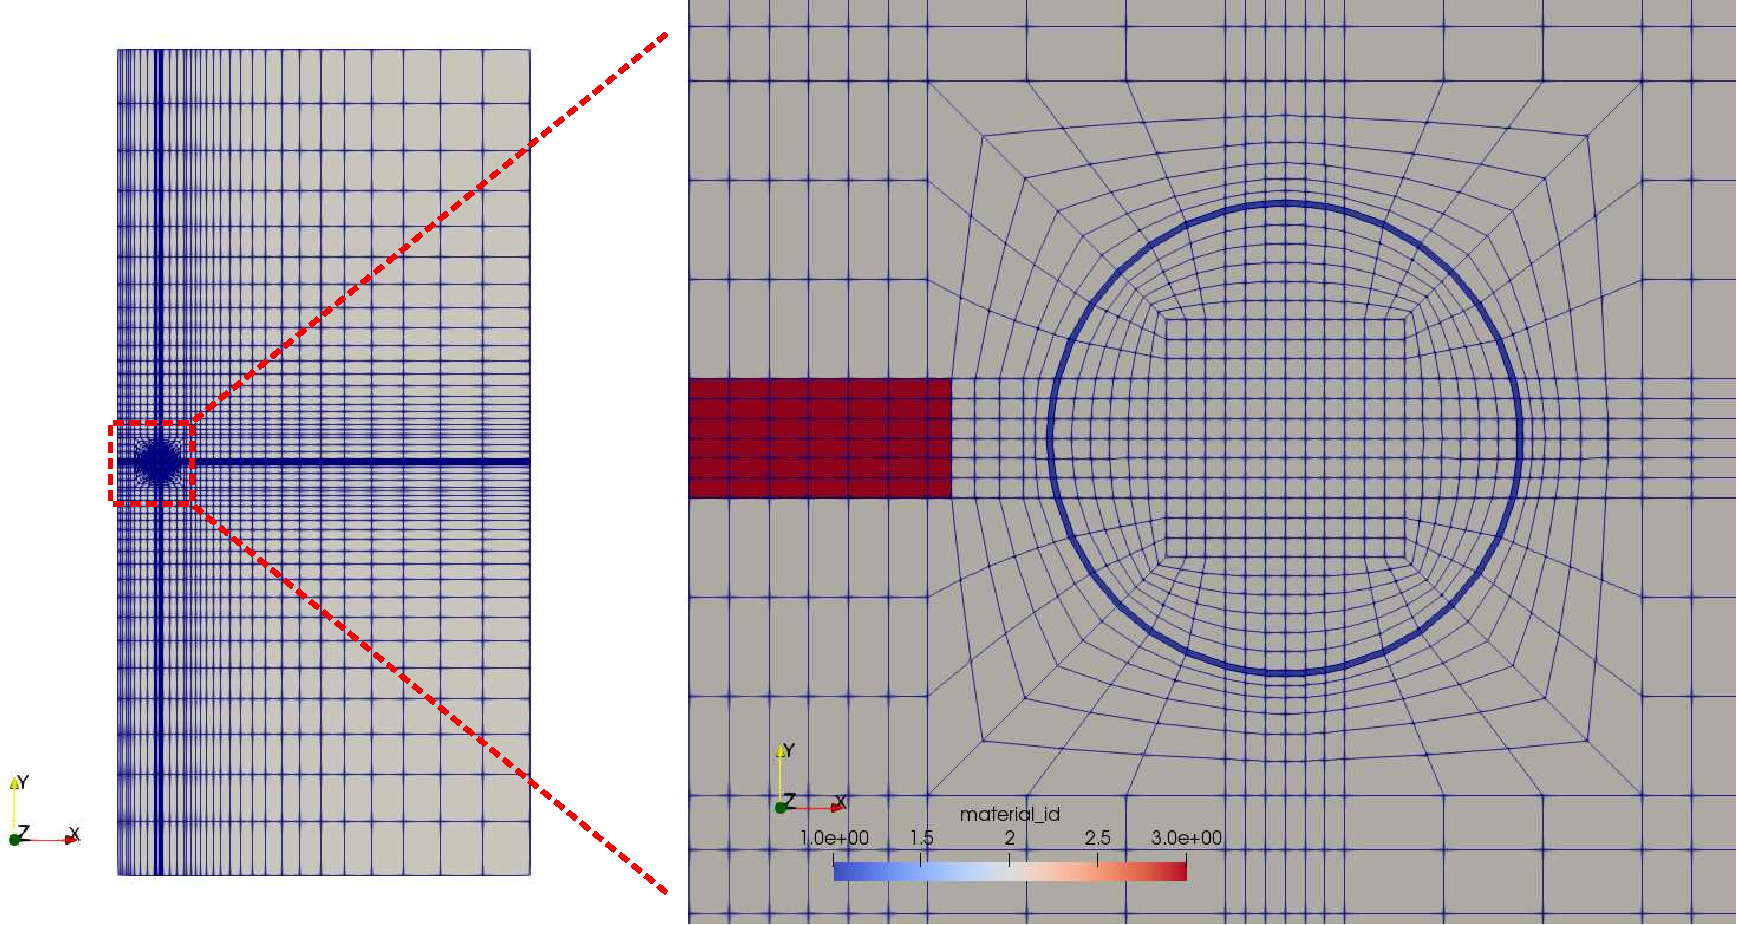
\includegraphics[width=0.7\textwidth]{2d_mesh.pdf}
\caption{Axisymmetric (2.5D) mesh geometry of toroid tube material modelled with surrounding free space (Red region: permanent magnet, blue region: torus magneto-elastic material and remaining region is the free space)}
\label{fig:1.2}
\end{figure}

\begin{figure}[htb]
\centering
\begin{subfigure}[b]{0.39\textwidth}
\centering
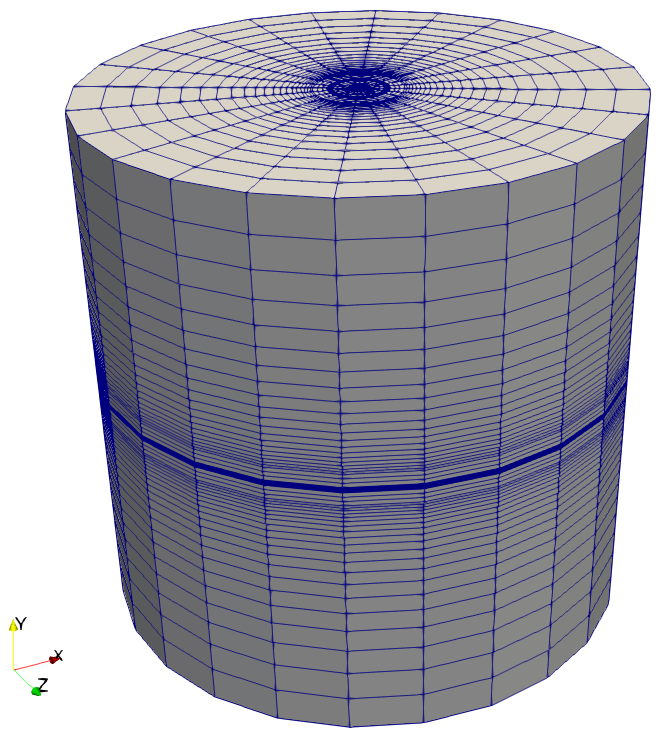
\includegraphics[width=0.9\textwidth]{3d_mesh_1.png}
\caption{3D mesh with free space}
\label{fig:1.3.1}
\end{subfigure}
\begin{subfigure}[b]{0.29\textwidth}
\centering
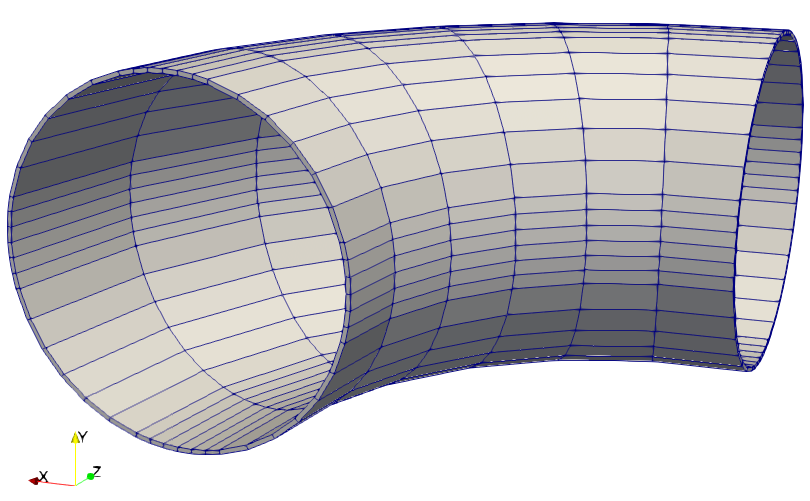
\includegraphics[width=0.85\textwidth]{3d_mesh_3.png}
\label{fig:1.3.2}
\caption{Cut section of toroid tube}
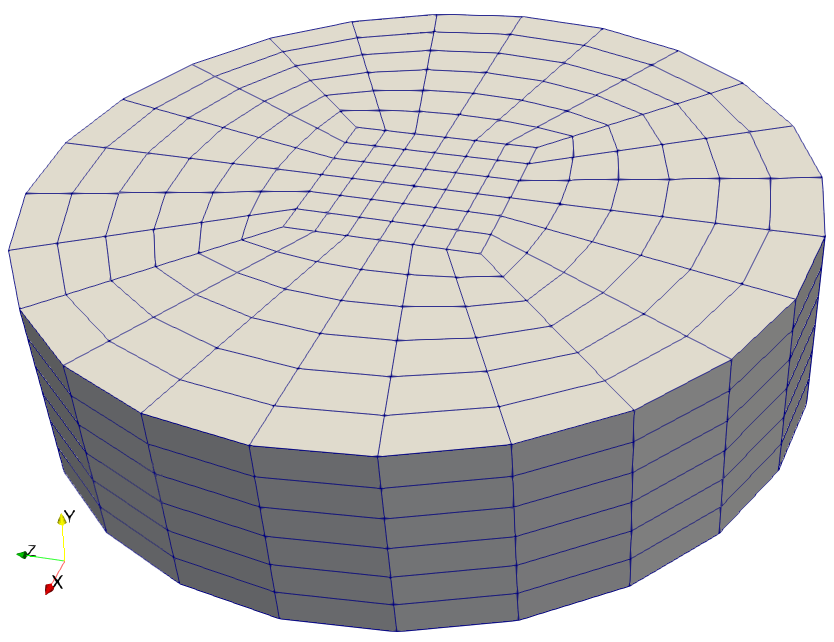
\includegraphics[width=0.85\textwidth]{3d_mesh_5.png}
\caption{Permanent magnet region}
\label{fig:1.3.4}
\end{subfigure}
\begin{subfigure}[b]{0.29\textwidth}
\centering
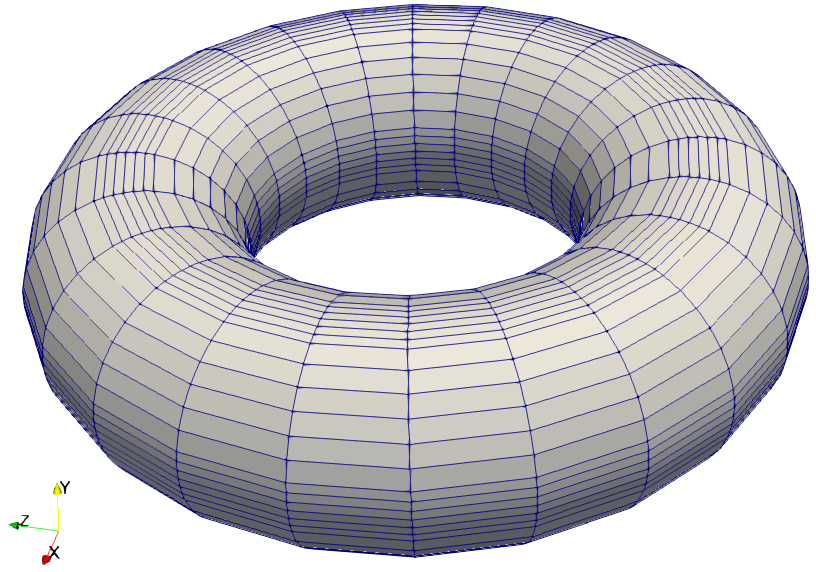
\includegraphics[width=0.75\textwidth]{3d_mesh_4.png}
\caption{Toroid tube}
\label{fig:1.3.3}
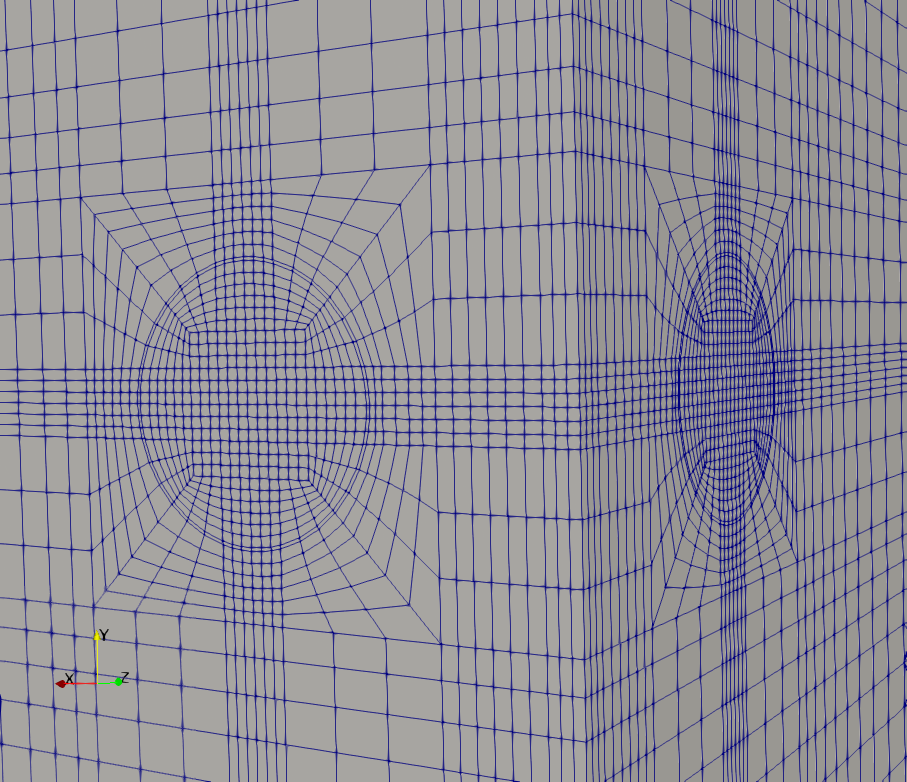
\includegraphics[width=0.75\textwidth]{3d_mesh_6.png}
\caption{Zoomed cross-section}
\label{fig:1.3.5}
\end{subfigure}
\caption{3D mesh geometry}
\label{fig:1.3}
\end{figure}

\section{Implementation details}
The open-source, high performance finite element library deal.II \cite{BangerthHartmannKanschat2007,dealII90} is used to model and simulate the magneto-elastic material with the free space around the toroid tube. Trilinos \cite{trilinos} vectors, matrices, preconditioners and solvers are used. The use of class  \href{https://www.dealii.org/current/doxygen/deal.II/classparallel_1_1shared_1_1Triangulation.html}{parallel$::$shared$::$Triangulation} for automatic partitioning of the domain among all the involved MPI processes (in parallel context) is done. To perform adaptive h-/p-refinement of the coarse mesh for a certain number of refinement iterations we employ the class \href{https://www.dealii.org/current/doxygen/deal.II/classhp_1_1DoFHandler.html}{hp$::$DoFHandler} to manage the distribution and enumeration of the degrees of freedom. In adaptive p-refinement we can have a different finite element on every cell of our mesh, whereas in h-refinement we can reduce the size of the mesh element where the error in solution is large. To mark the fraction of cells with largest error that would be then refined, we use the standard Kelly error estimator from the literature which is suitable and efficient for a large class of elliptic PDE's including the Laplace problem that we solve here. \par 
To generate a circulating magnetic field around the toroid tube we apply a linearly varying potential function to a region at the center of the body. This region of constrained degrees of freedom with the potential values has a shape of a rectangular box (in 2D), see the red box region in Figure \eqref{fig:1.2} or circular disk (in 3D) at the center of the domain, see Figure \eqref{fig:1.3.4}. The dimensions for this permanent magnet box/disk region to constrain the degrees of freedom and the linear potential function with which these DoFs will be constrained are user input parameters. \par 

\section{Numerical results}
\subsection{Validation of the axisymmetric formulation}
In order to validate the results of the axisymmetric formulation with the 3D simulation results we compute and compare an energy metric (scalar) contained in the magneto-elastic toroid tube material. The energy is computed as
\begin{equation}
E = \sum\limits_{cells \in \mathcal{B}_{tube}} \sum\limits_{q} \frac{1}{2} \mu_0 \ \mu_r \ \alpha \ \norm{-\nabla \phi(q)}^2 \ J \ w(q),
\end{equation}
where $\alpha$ is the co-ordinate transformation scaling factor which has the value of $2 \pi r$ for the axisymmetric formulation (2.5D) and 1 for the 3D simulation.\par 

\begin{figure}[t!]
\begin{subfigure}[t]{0.49\linewidth}
\centering
\resizebox{\linewidth}{!}{
\begin{tikzpicture}
\begin{semilogxaxis}[
xlabel = $\text{Number of cells}$,
ylabel = $\text{Total energy in membrane}$,
%grid =both,
%grid style=dashed,
%minor grid style ={gray!30},
%major grid style ={gray!30},
%width=0.8\linewidth,
legend pos=north east,
]
\addplot[
color=red,
mark=square,
line width=1pt,
]
table[x=NumberOfCells,y=TotalEnergy]{ref_sol_2d_energy_ncells.dat};
\addlegendentry{Total energy}
\end{semilogxaxis}
\end{tikzpicture}
}
\caption{Axisymmetric formulation}
\label{fig:1.4.1}
\end{subfigure}
\begin{subfigure}[t]{0.46\linewidth}
\centering
\resizebox{\linewidth}{!}{
\begin{tikzpicture} 
\begin{semilogxaxis}[
xlabel = $\text{Number of cells}$,
%ylabel = $\text{}$,
%grid =both,
%grid style=dashed,
%minor grid style ={gray!30},
%major grid style ={gray!30},
%width=0.8\linewidth,
legend pos=north east,
]
\addplot[
color=red,
mark=square,
line width=1pt,
]
table[x=NumberOfCells,y=TotalEnergy]{3d_3ref_energy_ncells.dat};
\addlegendentry{Total energy}
\end{semilogxaxis}
\end{tikzpicture}
}
\caption{3D simulation}
\label{fig:1.4.2}
\end{subfigure}
\caption{Total energy in the magneto-elastic toroid membrane for each refinement cycle}
\label{fig:1.4}
\end{figure} \par 

We observe the total energy in the magneto-elastic membrane due to the applied magneto-static magnetic scalar potential for the axisymmetric formulation for 4 refinement cycles in Figure \eqref{fig:1.4.1} and for the 3D simulation for 3 refinement cycles in Figure \eqref{fig:1.4.2} (less number of refinement cycles due to memory bottleneck with vastly growing number of cells). 4 MPI processes were employed to obtain the results. As can be observed, the total energy by both the approaches are comparable with a maximum relative error of 15\%. We observe a convergence in the total energy with each h-adaptive mesh refinement cycle. High computational cost for the 3D simulation is clearly observable when comparing the number of cells in the domain against the number of cells in axisymmetric (2.5D) simulation result. \par 

\subsection{Experiment with the permanent magnet region and the applied potential}
We carried out a study on the size of the permanent magnet region in which we constrain the DoFs to a linearly varying magnetic potential. This region, as explained earlier, is a rectangular box in 2D/circular disk in 3D. In addition to studying the behaviour of results on the dependence of the size of this magnet region, we also experimented with the change in the linear potential function values. The magnet region dimensions (length and height) and the potential function to apply are user input parameters and are varied in this study. This experiment was carried out for the axisymmetric (2.5D) model only.\par 

\begin{figure}[h]
\centering
\begin{subfigure}{0.32\textwidth}
\centering
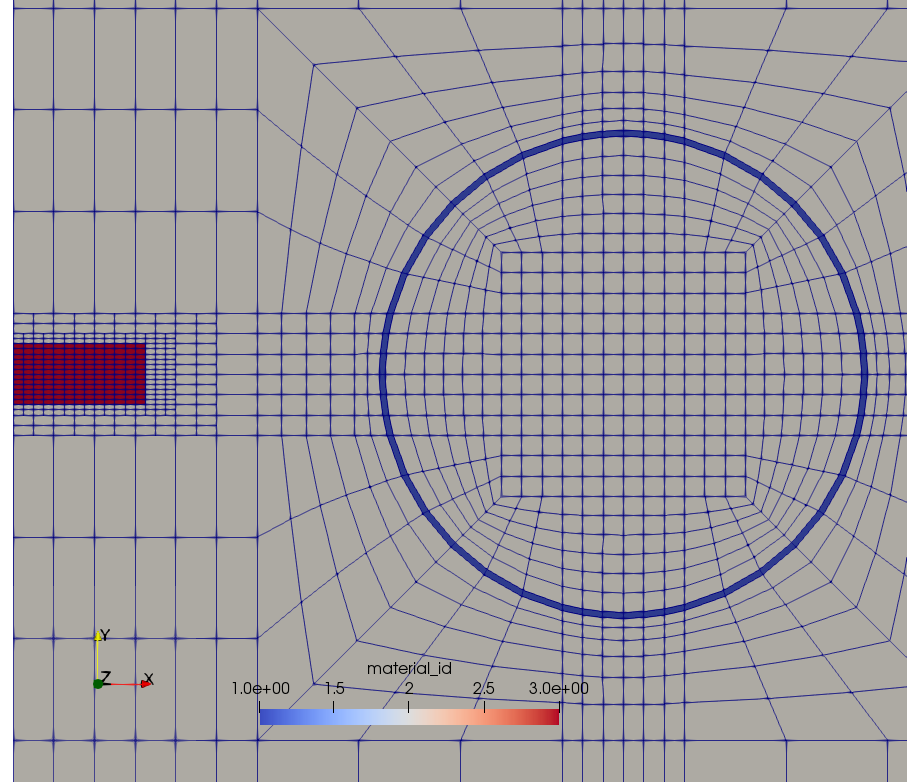
\includegraphics[width=0.87\textwidth]{magnet_x_p.png}
\caption{\scriptsize Magnet x=0.11,y=0.0255 \\(red block)}
\label{fig:1.5.1}
\end{subfigure}
\begin{subfigure}{0.33\textwidth}
\centering
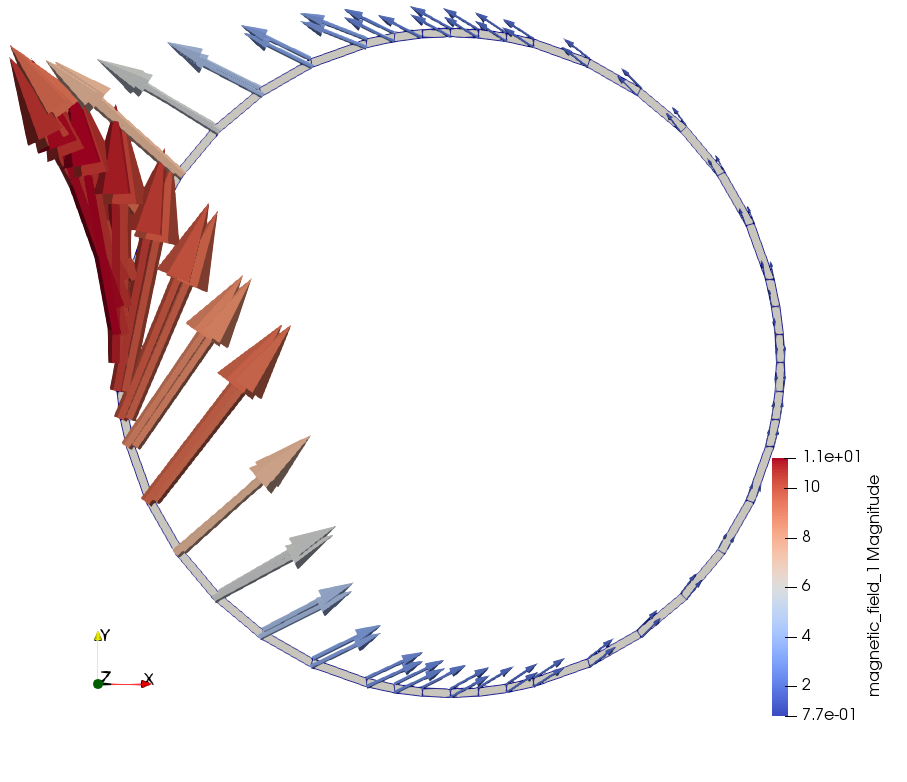
\includegraphics[width=0.85\textwidth]{x_p.png}
\caption{\scriptsize Pot. diff.= 1000 \\ Max. $\mathbbm{h}$= 1.1e+01, Min. $\mathbbm{h}$= 7.7e-01}
\label{fig:1.5.2}
\end{subfigure}
\begin{subfigure}{0.33\textwidth}
\centering
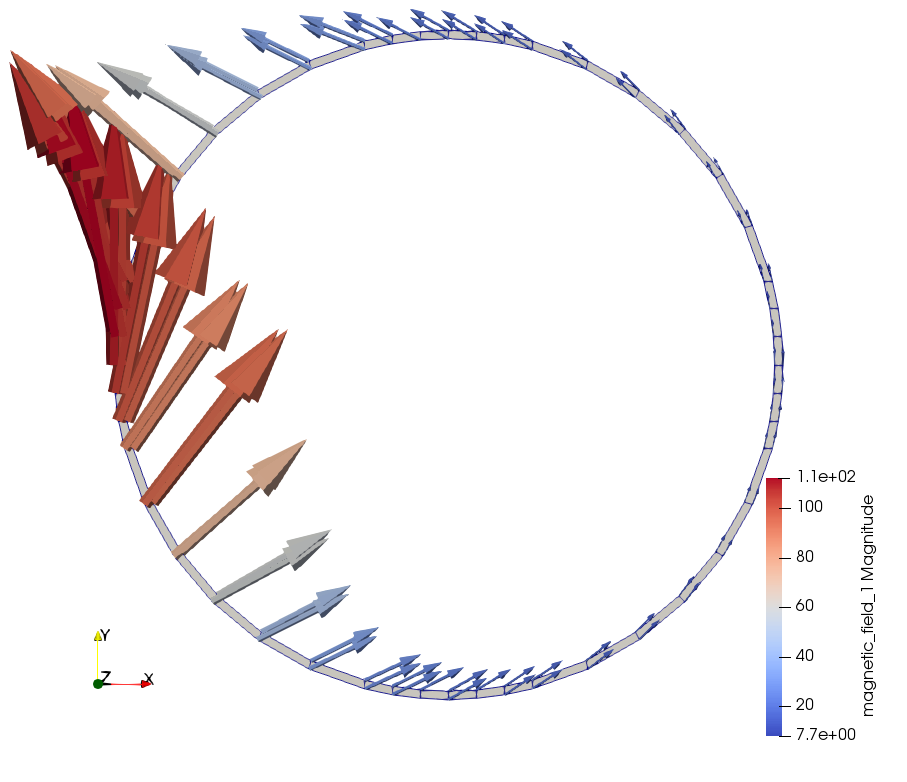
\includegraphics[width=0.85\textwidth]{x_10p.png}
\caption{\scriptsize Pot. diff.= 10000 \\ Max. $\mathbbm{h}$= 1.1e+02, Min. $\mathbbm{h}$= 7.7e+00}
\label{fig:1.5.3}
\end{subfigure}
\vspace{0.5cm}
\begin{subfigure}{0.32\textwidth}
\centering
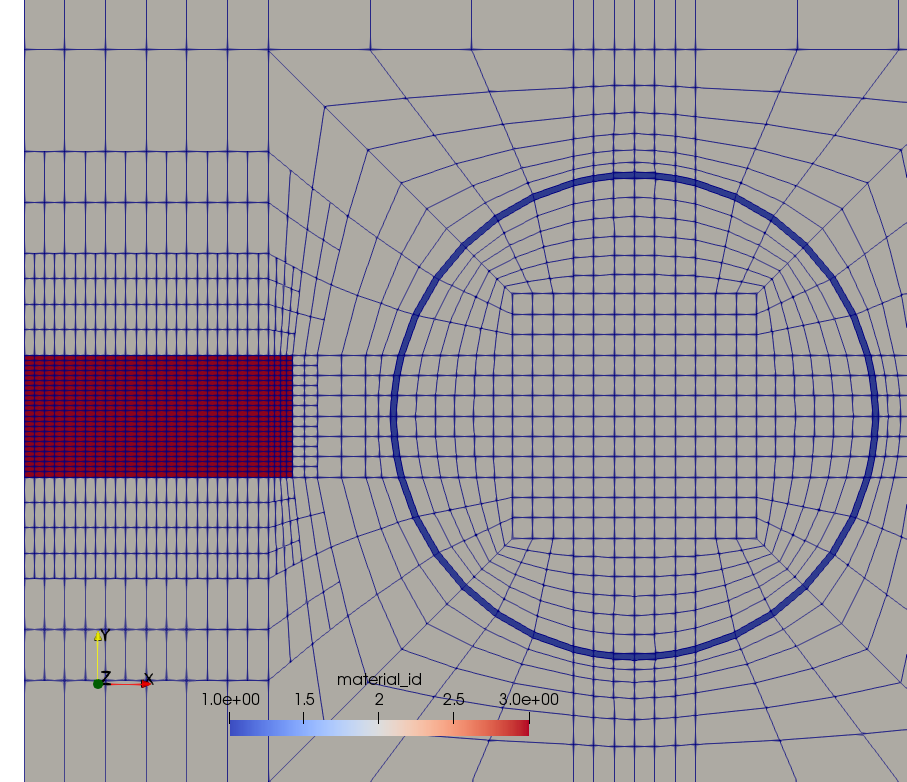
\includegraphics[width=0.87\textwidth]{magnet_2x_p.png}
\caption{\scriptsize Magnet x=0.22,y=0.051 \\(red block)}
\label{fig:1.5.4}
\end{subfigure}
\begin{subfigure}{0.33\textwidth}
\centering
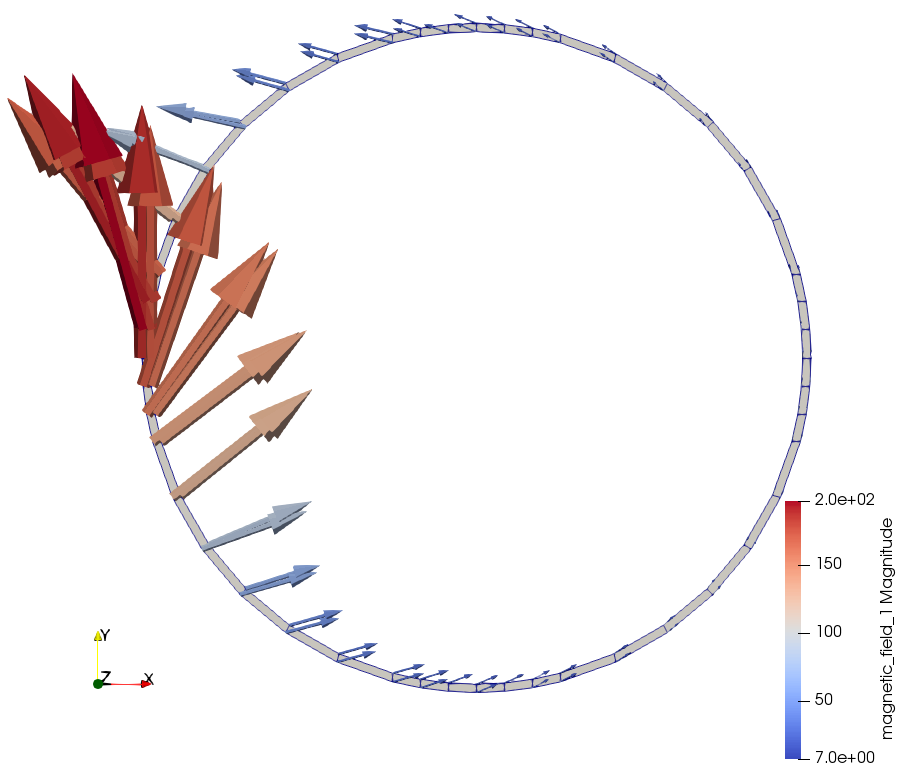
\includegraphics[width=0.85\textwidth]{2x_p.png}
\caption{\scriptsize Pot. diff.= 1000 \\ Max. $\mathbbm{h}$= 2.0e+02, Min. $\mathbbm{h}$= 7.0e+00}
\label{fig:1.5.5}
\end{subfigure}
\begin{subfigure}{0.33\textwidth}
\centering
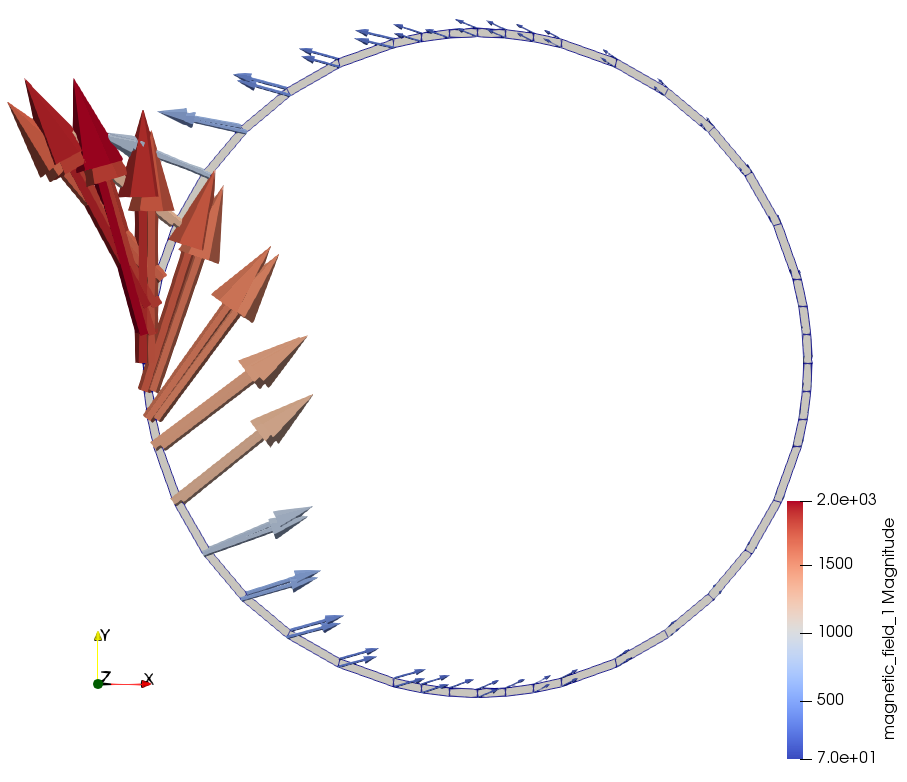
\includegraphics[width=0.86\textwidth]{2x_10p.png}
\caption{\scriptsize Pot. diff.= 10000 \\ Max. $\mathbbm{h}$= 2.0e+03, Min. $\mathbbm{h}$= 7.0e+01}
\label{fig:1.5.6}
\end{subfigure}
\caption{Effect of magnet size and applied magnetic potential in torus membrane field}
\label{fig:1.5}
\end{figure}

In the above figures we observe the resulting magnetic field $\mathbbm{h}$ for the input magnet region and applied magnetic potential parameters. Figure \eqref{fig:1.5.4} has double the magnet size when compared to the magnet size in Figure \eqref{fig:1.5.1}. When comparing the results for this effect of increased magnet size, we observe in Figure \eqref{fig:1.5.5} an increase in the magnitude of the magnetic field against the result in Figure \eqref{fig:1.5.2}. In Figure \eqref{fig:1.5.3} we increase the applied magnetic potential ten times of that used in the result for Figure \eqref{fig:1.5.2} keeping the size of the permanent magnet region the same. We observe the magnetic field has proportionally increased by same magnitude. Combined increase in the magnet region (twice as original size) and magnetic potential (10 times the original value) we observe the magnetic field has increased by a significantly large magnitude, see Figure \eqref{fig:1.5.6}. It is important to observe that the direction of magnetic field near the torus membrane did not change in any of the variation case. The aim of this study is to find appropriate values for the above three parameters such that we have a tangential magnetic field in the torus membrane to satisfy the curl free condition as given in Equation \eqref{eq:1.2}. \par 

The results with appropriately chosen values of these parameters for future work are depicted in Figure \eqref{fig:1.6} and \eqref{fig:1.7}.

\begin{figure}[h]
\centering
\begin{subfigure}{0.49\textwidth}
\centering
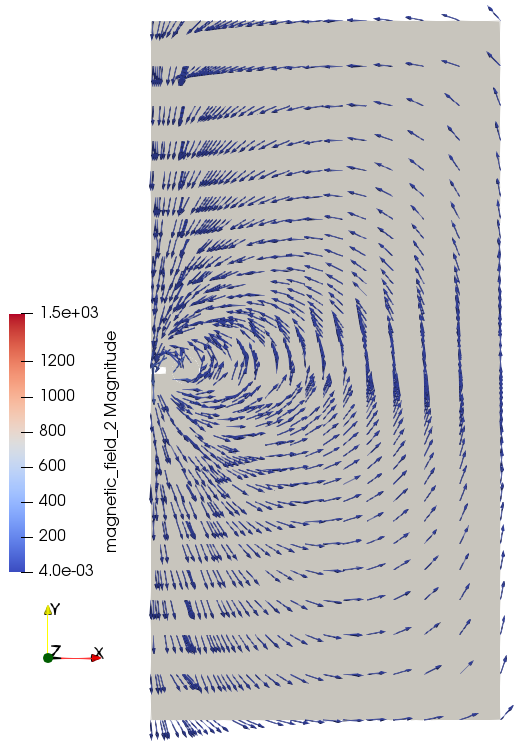
\includegraphics[width=0.55\textwidth]{2d_free_space.png}
\caption{Magnetic field in free space}
\label{fig:1.6.1}
\end{subfigure}
\begin{subfigure}{0.49\textwidth}
\centering
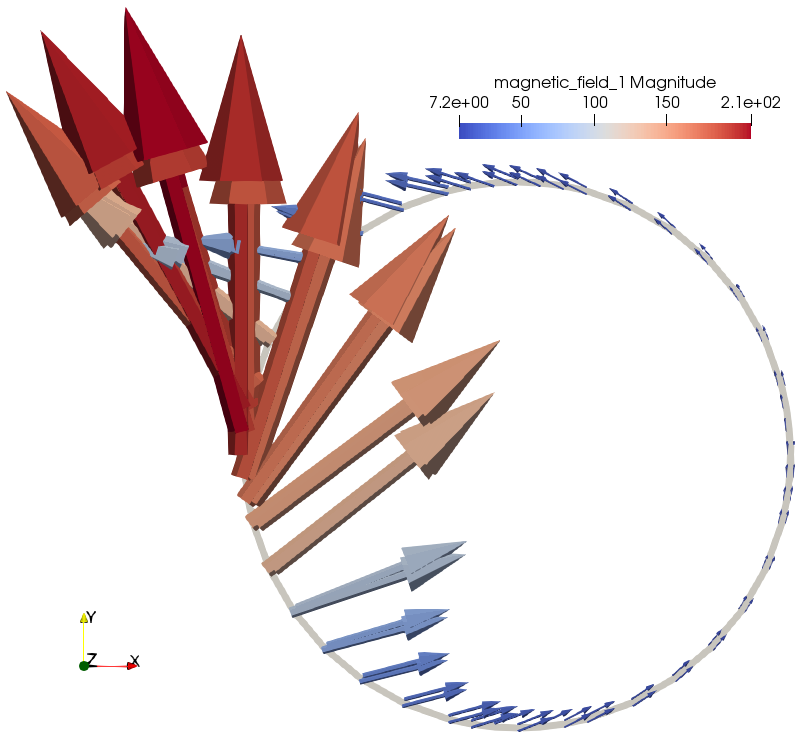
\includegraphics[width=0.85\textwidth]{2d_toroid_field_2.png}
\caption{Magnetic field in torus membrane}
\label{fig:1.6.2}
\end{subfigure}
\caption{Axisymmetric (2.5D) formulation}
\label{fig:1.6}
\end{figure}

\begin{figure}[h]
\centering
\begin{subfigure}{0.49\textwidth}
\centering
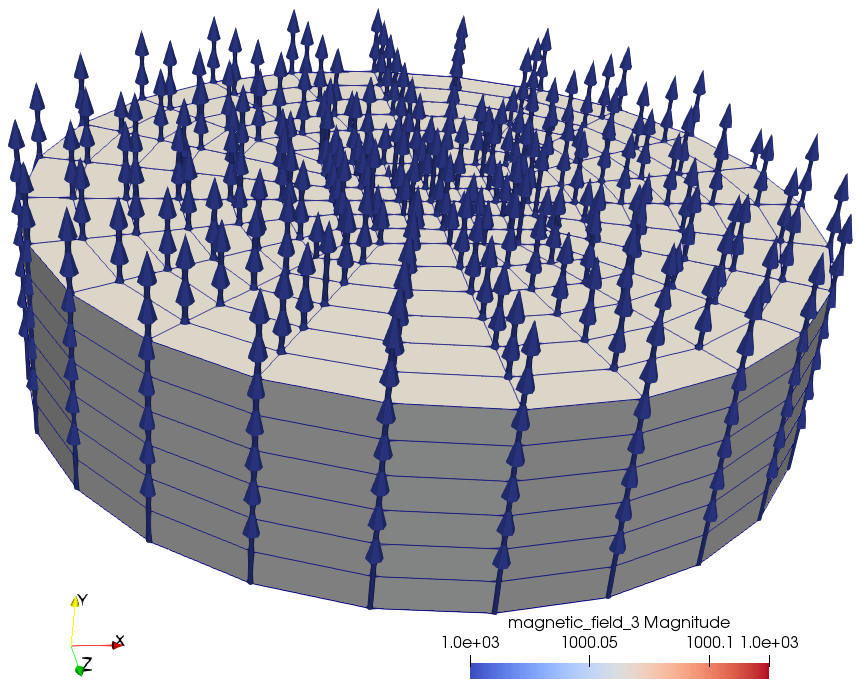
\includegraphics[width=0.8\textwidth]{3d_1quar_magnet_field.png}
\caption{Magnetic field in permanent magnet}
\label{fig:1.7.1}
\end{subfigure}
\begin{subfigure}{0.49\textwidth}
\centering
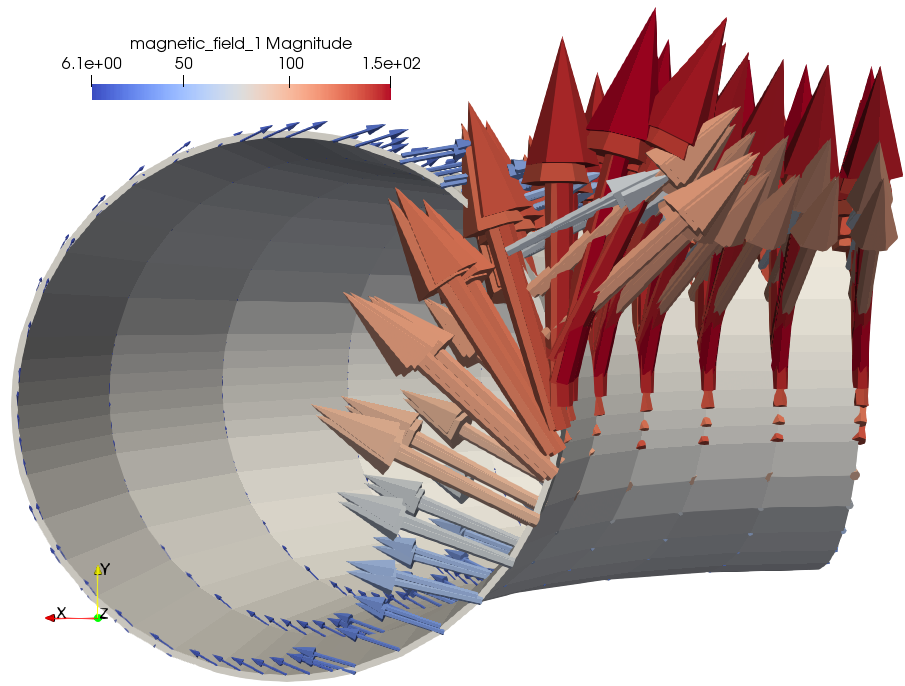
\includegraphics[width=0.85\textwidth]{3d_1quar_toroid_field_2.png}
\caption{Magnetic field in torus membrane}
\label{fig:1.7.2}
\end{subfigure}
\caption{3D simulation}
\label{fig:1.7}
\end{figure}

\chapter{Quasi-static finite-strain compressible elasticity}

\section{Kinematics}
Consider a continuum body $\mathcal{B}_0$ in a three dimensional Euclidean space. Let any point in this reference configuration $\mathcal{B}_0$ be identified by the position vector $\mathbf{X}$. The configuration after some time $t > 0$ is termed as deformed configuration $\mathcal{B}_t$ and the corresponding position vector $\mathbf{x}$ is given by a non-linear one-to-one deformation map $\mathbf{x} = \bm{\varphi} (\mathbf{X}, t)$. The material description of the displacement of the particle at the position $\mathbf{X}$ is defined as
\begin{equation}
\mathbf{u}(\mathbf{X}, t) := \mathbf{x}(\mathbf{X}, t) - \mathbf{X}.
\end{equation}
A tensor $\mathbf{F}$ which describes the deformation process locally relates the tangent vectors of reference and current configuration to each other. It maps a material line element of the reference configuration $\bm{\mathrm{d}}\mathbf{X}$ in $\mathcal{B}_0$ to a line element $\bm{\mathrm{d}\mathbf{x}}$ in $\mathcal{B}_t$ as 
\begin{equation}
\bm{\mathrm{d}\mathbf{x}} = \mathbf{F} \cdot \bm{\mathrm{d}\mathbf{X}}.
\end{equation} 
This tensor $\mathbf{F}$ is called the deformation gradient and is the material gradient of the motion defined as
\begin{equation}
\mathbf{F}(\mathbf{X}, t) := \dfrac{\partial \bm{\varphi}(\mathbf{X}, t)}{\partial \mathbf{X}} = \nabla_0 \mathbf{x}(\mathbf{X}, t) = \mathbf{I} + \nabla_0 \mathbf{u}.
\label{eq:2.3}
\end{equation}
The gradient w.r.t. the reference configuration $\mathcal{B}_0$ is denoted as $\nabla_0$ and the gradient w.r.t. the deformed configuration $\mathcal{B}_t$ be denoted as $\nabla$ and are related as 
\begin{equation}
\nabla \{ \cdot \} = \dfrac{\partial \{ \cdot \} }{\partial \mathbf{x}} = \dfrac{\partial \{ \cdot \} }{\partial \mathbf{X}} \cdot \dfrac{\partial \mathbf{X}}{\partial \mathbf{x}} = \nabla_0 \{ \cdot \} \cdot \mathbf{F}^{-1}.
\end{equation} 
The transformation of surface area elements between $\mathcal{B}_0$ and $\mathcal{B}_t$ is given by the \textbf{Nanson's formula}
\begin{equation}
\bm{\mathrm{d}}\mathbf{a} = \mathbf{n} \cdot \mathrm{d}a = J \ \mathbf{F}^{-T} \cdot \mathbf{N} \mathrm{d}A = J \ \mathbf{F}^{-T} \cdot \bm{\mathrm{d}}\mathbf{A},
\end{equation}
where $\mathbf{n}$ is the normal vector of the surface in $\mathcal{B}_t$, $\mathbf{N}$ is the normal vector in $\mathcal{B}_0$ and $\mathrm{d}a$ and $\mathrm{d}A$ are the corresponding area elements. The determinant of the deformation gradient, known as the Jacobian, $J(\mathbf{X}, t) := \text{det} \mathbf{F}(\mathbf{X}, t) > 0$ (non-negative to avoid material self-penetration) maps the volume elements in material and spatial configurations $\mathrm{d}V$ and $\mathrm{d}v$, respectively, as 
\begin{equation}
\mathrm{d}v = J(\mathbf{X}, t) \ \mathrm{d}V.
\end{equation} 
The strain tensor in the material configuration $\mathcal{B}_0$ is defined as
\begin{equation}
\mathbf{E} := \frac{1}{2} (\mathbf{F}^T \cdot \mathbf{F} - \mathbf{I}) = \frac{1}{2} (\mathbf{C} - \mathbf{I}),
\end{equation}
and is called as the Green-Lagrange strain tensor. The tensor $\mathbf{C}:= \mathbf{F}^T \cdot \mathbf{F}$ is known as the right Cauchy-Green deformation tensor which expresses the square of the line element $\bm{\mathrm{d}}\mathbf{x}$ by the material line element $\bm{\mathrm{d}}\mathbf{X}$ as $\bm{\mathrm{d}}\mathbf{x} \cdot \bm{\mathrm{d}}\mathbf{x} = \bm{\mathrm{d}}\mathbf{X} \cdot \mathbf{C} \cdot \bm{\mathrm{d}}\mathbf{X}$. $\mathbf{C}$ is \textit{symmetric} and \textit{positive definite} at each $\mathbf{X} \in \mathcal{B}_0$. Thus the Green-Lagrange strain $\mathbf{E}$ is also symmetric. The strain $\mathbf{E}$ describes the change of the square of the line elements from $\mathcal{B}_0$ to $\mathcal{B}_t$. Using the definition of $\mathbf{F}$ from \Cref{eq:2.3}, we can express the Green-Lagrange strain in terms of the displacement gradient as 
\begin{equation}
\mathbf{E} = \frac{1}{2} ( \nabla_0 \mathbf{u} + [\nabla_0 \mathbf{u}]^T + [\nabla_0 \mathbf{u}]^T \cdot \nabla_0 \mathbf{u} ).
\end{equation}

\section{Kinetics}
The Cauchy stress theorem states that the Cauchy traction $\mathbf{t}$ acting on an infinitesimal surface element $\mathrm{d}a$ in the current configuration $\mathcal{B}_t$ is the product of the Cauchy stress tensor $\bm{\sigma}$, a spatial quantity, and the outward unit normal vector to the surface $\mathrm{d}a$ as 
\begin{equation}
\mathbf{t}(\mathbf{x}, t, \mathbf{n}) = \bm{\sigma}(\mathbf{x}, t) \cdot \mathbf{n}.
\end{equation}
Following the result of balance of angular momentum, it is known that the Cauchy stress tensor is symmetric. Similar relation in the material configuration is given as 
\begin{equation}
\mathbf{T}(\mathbf{X}, t, \mathbf{N}) = \mathbf{P}(\mathbf{X}, t) \cdot \mathbf{N},
\end{equation}
where $\mathbf{T}$ is the first Piola-Kirchhoff traction acting on an infinitesimal surface element $\mathrm{d}A$ and $\mathbf{P}$ is the first Piola-Kirchhoff stress tensor. $\mathbf{P}$ is a two-point tensor indicating that it is neither a material or a spatial quantity. The first Piola-Kirchhoff stress tensor is related to the Cauchy stress tensor as 
\begin{equation}
\mathbf{P} = J \ \bm{\sigma} \cdot \mathbf{F}^{-T}.
\end{equation}
The Cauchy traction $\mathbf{t}$ and the first Piola-Kirchhoff traction $\mathbf{T}$ are related as 
\begin{equation}
\mathbf{T} \ \bm{\mathrm{d}}\mathbf{A} = \mathbf{t} \ \bm{\mathrm{d}}\mathbf{a},
\end{equation}
such that
\begin{equation}
\int\limits_{\mathcal{B}_0} \left[ \mathbf{P} \cdot \mathbf{N} \right] \mathrm{d}A = \int\limits_{\mathcal{B}_0} \left[ J \ \bm{\sigma} \cdot \mathbf{F}^{-T} \right] \cdot \mathbf{N} \ \mathrm{d}A = \int\limits_{\mathcal{B}_0} \bm{\sigma} \cdot \left[ J \ \mathbf{F}^{-T} \cdot \mathbf{N} \right] \mathrm{d}A \stackrel{\text{Nanson's}}{=} \int\limits_{\mathcal{B}_t} \bm{\sigma} \cdot \mathbf{n} \ \mathrm{d}a.
\end{equation}
A completely material stress measure is also introduced known as the second Piola-Kirchhoff stress tensor given as
\begin{equation}
\mathbf{S} = \mathbf{F}^{-1} \cdot \mathbf{P}.
\end{equation}
The second Piola-Kirchhoff stress tensor is symmetric tensor.

\section{Constitutive material model}
\label{sec:const_law}
The kinematical relations and balance laws are not sufficient to solve a boundary value or initial value problem. For a complete set of equations, a constitutive equation needs to be formulated which can appropriately characterize the material response of a body. \par 

Hyperelastic materials are the purely elastic material behaviour under the assumption of the so-called Green elasticity. The material response is characterised by a Helmholtz free energy function $\Psi = \Psi(\mathbf{F}) = \Psi(\mathbf{C}) $ which serves as a potential for the stress. $\Psi$ describes the strain energy stored in the body and hence also known as the strain energy function (S.E.F.). When S.E.F. is described in terms of the right Cauchy-Green tensor $\mathbf{C}$ then the isotropic hyperelastic material response is 
\begin{equation}
\mathbf{S} = 2 \dfrac{\partial \Psi (\mathbf{C})}{\partial \mathbf{C}}.
\end{equation}
A Neo-Hookean solid is a hyperelastic material model that can be used for predicting the non-linear behaviour of materials undergoing large deformations under loads. The Neo-Hookean material model is usable for plastics and rubber-like materials. The S.E.F. corresponding to a compressible Neo-Hookean material is given as
\begin{equation}
\Psi \equiv \dfrac{\mu}{2} [\mathbf{C} : \mathbf{I} - \mathbf{I} : \mathbf{I} - 2 \ln J] + \dfrac{\lambda}{2} (\ln J)^2,
\label{eq:2.2}
\end{equation}
where $\mu$ and $\lambda$ are the Lam\'e parameters. For the considered S.E.F. for the Neo-Hookean material as stated in \Cref{eq:2.2}, the second Piola-Kirchhoff stress is:
\begin{align}
\mathbf{S} = 2 \left\{ \dfrac{\mu}{2} \left[\dfrac{\partial (\mathbf{C} : \mathbf{I})}{\partial \mathbf{C}} - 0 - 2 \dfrac{\partial \ln J}{\partial \mathbf{C}}\right] + \dfrac{\lambda}{2} \dfrac{\partial (\ln J)^2}{\partial \mathbf{C}} \right\}
\end{align}
Employing the chain rule for the intermediate partial derivatives
\begin{align}
\dfrac{\partial (\mathbf{C} : \mathbf{I})}{\partial \mathbf{C}} &= \mathbf{I} \label{eq:2.4.1} \\ 
\dfrac{\partial \ln J}{\partial \mathbf{C}} &= \dfrac{1}{J} \dfrac{\partial J}{\partial \mathbf{C}} \label{eq:2.4.2} \\ 
\dfrac{\partial (\ln J)^2}{\partial \mathbf{C}} &= 2 \dfrac{\partial \ln J}{\partial \mathbf{C}} = 2 \dfrac{1}{J} \dfrac{\partial J}{\partial \mathbf{C}}
\label{eq:2.4.3}
\end{align}
The partial derivative of the Jacobian w.r.t. the right Cauchy-Green deformation tensor is given as \cite[see][page 46 Equation (3.124)]{Wriggers2008}:
\begin{equation}
\dfrac{\partial J}{\partial \mathbf{C}} = \dfrac{1}{2} \ J \ \mathbf{C}^{-1}.
\label{eq:2.5}
\end{equation}
Rearranging the terms with the use of the results from \Crefrange{eq:2.4.1}{eq:2.4.3} and \Cref{eq:2.5}, we have
\begin{equation}
\mathbf{S} = \mu \mathbf{I} - \left[ \mu - \lambda \ln J \right] \mathbf{C}^{-1}.
\label{eq:2.6}
\end{equation}
The fourth-order elasticity tensor in the material description is defined as 
\begin{equation}
\mathfrak{C} := 2 \dfrac{\partial \mathbf{S}(\mathbf{C})}{\partial \mathbf{C}} = 4 \dfrac{\partial^2 \Psi (\mathbf{C})}{\partial \mathbf{C} \otimes \partial \mathbf{C}}.
\label{eq:2.6.2}
\end{equation}
Using the derived form for the second Piola-Kirchhoff stress from \Cref{eq:2.6}, we have
\begin{equation}
\mathfrak{C} = \left[ 2 \lambda \ln J - 2 \mu \right]\dfrac{\partial \mathbf{C}^{-1}}{\partial \mathbf{C}} + \lambda \mathbf{C}^{-1} \otimes \mathbf{C}^{-1},
\end{equation}
with the standard result \cite[see][page 519]{Wriggers2008}
\begin{equation}
\dfrac{\partial C^{-1}_{IJ}}{\partial C_{KL}} := \dfrac{-1}{2} \left[ C^{-1}_{IK} \ C^{-1}_{LJ} + C^{-1}_{IL} \ C^{-1}_{KJ} \right].
\end{equation}
The fourth-order elasticity tensor for hyperelastic materials possess both major and minor symmetries, i.e. $\mathfrak{C} = C_{IJKL} = C_{KLIJ} = C_{JIKL} = C_{IJLK}$.

\section{Weak formulation in the referential configuration}
For the analysis of (non-)linear initial boundary value problems in continuum theory, a coupled system of partial differential equations needs to be solved consisting of kinematical relations, the local balance law of linear momentum and the constitutive equations. The description of the strong form of these equations, here, will be with respect to the initial configuration of the bodies. 
\begin{align*}
\text{Kinematics}&: \ \mathbf{F}, \ \mathbf{E} = \dfrac{1}{2} (\mathbf{F}^T \cdot \mathbf{F} - \mathbf{I}) \\
\text{Equilibrium}&: \ \text{Div}(\mathbf{F} \cdot \mathbf{S}) + \mathbf{b}^p = \mathbf{0} \\
\text{Constitutive equation}&: \ \mathbf{S} = 2\dfrac{\partial \Psi}{\partial \mathbf{C}}.
\end{align*}
In addition the boundary conditions for the displacements have to be imposed on $\partial \mathcal{B}_{0,u}$ and for tractions on the boundary $\partial \mathcal{B}_{0,t}$, with $\partial \mathcal{B}_{0,u} \cap \partial \mathcal{B}_{0,t} = \emptyset$.
\begin{equation*}
\text{Boundary conditions} : \ \mathbf{u} = \mathbf{u}^p \ \text{on} \ \partial \mathcal{B}_{0,u} \ \& \ \mathbf{F} \cdot \mathbf{S} \cdot \mathbf{N} = \mathbf{t}^p \ \text{on} \ \partial \mathcal{B}_{0,t}.
\end{equation*}
$\mathbf{b}^p$ is the prescribed body force and $\mathbf{t}^p$ is the prescribed traction force per unit area. The finite element method, which is based on a variational formulation of the equations, can be fulfilled in a weak sense minimizing the error of the finite element approximation for arbitrarily chosen test functions. Let $\mathbf{u}^h$ be the approximation of the exact solution $\mathbf{u}$. Since the approximate solution is usually not the same as the exact solution, an error $\mathbf{R}$ will occur when satisfying the strong form of the above equations.
\begin{equation}
\text{Div}(\mathbf{F}(\mathbf{u}^h) \cdot \mathbf{S}) + \mathbf{b}^p = \mathbf{R}.
\end{equation}
The error $\mathbf{R}$ will be minimized in a weak sense by multiplying the residual by a vector-valued weighting function $\bm{\eta}$ and integrating the residual over the whole domain. This vector-valued function $\bm{\eta}$ is called as test function. Thus, we have
\begin{equation}
\int\limits_{\mathcal{B}_0} \text{Div}(\mathbf{F} \cdot \mathbf{S}) \cdot \bm{\eta} \ \mathrm{d}V + \int\limits_{\mathcal{B}_0} \mathbf{b}^p \cdot \bm{\eta} \ \mathrm{d}V = 0 \ \ \forall \bm{\eta}.
\label{eq:2.7}
\end{equation}
By doing integration by parts of the first term in \Cref{eq:2.7}, with the application of divergence theorem and the boundary conditions for displacement and traction, we have the weak form as 
\begin{equation}
\int\limits_{\mathcal{B}_0} \mathbf{F} \cdot \mathbf{S} \cdot \nabla_0 \bm{\eta} \ \mathrm{d}V - \int\limits_{\mathcal{B}_0} \mathbf{b}^p \cdot \bm{\eta} \ \mathrm{d}V - \int\limits_{\mathcal{\partial B}_{0,t}} \mathbf{t}^p \cdot \bm{\eta} \ \mathrm{d}A = 0 \ \ \forall \bm{\eta}.
\label{eq:2.8}
\end{equation}
Simplifying the first term in \Cref{eq:2.8} using the fact that the scalar product of a symmetrical tensor with an anti-symmetrical tensor is zero, we have
\begin{align}
\mathbf{F} \cdot \mathbf{S} \cdot \nabla_0 \bm{\eta} = \mathbf{S} \cdot \mathbf{F}^T \cdot \nabla_0 \bm{\eta} = \mathbf{S} \cdot \dfrac{1}{2} (\mathbf{F}^T \cdot \nabla_0 \bm{\eta} + \nabla_0^T \bm{\eta} \cdot \mathbf{F}) = \mathbf{S} \cdot \delta \mathbf{E}.
\label{eq:2.9}
\end{align}
$\delta \mathbf{E}$ denotes the variation of the Green-Lagrange strain tensor which is obtained as the directional derivative
\begin{align}
D\mathbf{E} \cdot \bm{\eta} &= \dfrac{1}{2} \dfrac{\mathrm{d}}{\mathrm{d\alpha}} \left[ \mathbf{F}^T (\bm{\varphi} + \alpha \bm{\eta}) \cdot \mathbf{F}(\bm{\varphi} + \alpha \bm{\eta}) - \mathbf{I} \right] \Big|_{\alpha = 0} \nonumber \\
&= \dfrac{1}{2} \left[ \dfrac{\partial \mathbf{F}^T (\bm{\varphi} + \alpha \bm{\eta})}{\partial \alpha} \cdot \mathbf{F}(\bm{\varphi} + \alpha \bm{\eta}) + \mathbf{F}^T (\bm{\varphi} + \alpha \bm{\eta}) \cdot \dfrac{\partial \mathbf{F}(\bm{\varphi} + \alpha \bm{\eta})}{\partial \alpha} - \dfrac{\partial \mathbf{I}}{\partial \alpha} \right] \Bigg|_{\alpha = 0} \nonumber \\
&= \dfrac{1}{2} \left[ \dfrac{\partial \left[ \mathbf{I} + \nabla_0^T (\bm{\varphi} + \alpha \bm{\eta}) \right]}{\partial \alpha} \cdot \mathbf{F}(\bm{\varphi} + \alpha \bm{\eta}) + \mathbf{F}^T (\bm{\varphi} + \alpha \bm{\eta}) \cdot \dfrac{\partial \left[ \mathbf{I} + \nabla_0 (\bm{\varphi} + \alpha \bm{\eta}) \right]}{\partial \alpha} - \mathbf{0} \right] \Bigg|_{\alpha = 0} \nonumber \\
&\stackrel{\alpha = 0}{=} \dfrac{1}{2} \left[ (\nabla_0 \bm{\eta})^T \cdot \mathbf{F} (\bm{\varphi}) + \mathbf{F}^T (\bm{\varphi}) \cdot \nabla_0 \bm{\eta} \right] = \delta \mathbf{E}.
\label{eq:2.10}
\end{align}
Using the result of \Cref{eq:2.9} and \Cref{eq:2.10} in \Cref{eq:2.8}, we have
\begin{equation}
G(\bm{\varphi},\bm{\eta}):= \int\limits_{\mathcal{B}_0} \mathbf{S} \cdot \delta \mathbf{E} \ \mathrm{d}V - \int\limits_{\mathcal{B}_0} \mathbf{b}^p \cdot \bm{\eta} \ \mathrm{d}V - \int\limits_{\mathcal{\partial B}_{0,t}} \mathbf{t}^p \cdot \bm{\eta} \ \mathrm{d}A = 0 \ \ \forall \bm{\eta}.
\label{eq:2.11}
\end{equation}
The first term in \Cref{eq:2.11} denotes the internal virtual work performed by the body. The last two terms are the virtual work of the applied traction and the inertia load.

\subsection{Variational principles}
\textbf{Principle of stationary potential energy}: The S.E.F. for the considered hyperelastic material model describes the stored energy in the continuum body. Based on this S.E.F. we can find the equilibrium configuration by the principle of minimum potential energy. The total potential energy of the system $\Pi$ is the sum of the internal and external potential energies and is defined as 
\begin{equation}
\Pi = \Pi_{int} + \Pi_{ext},
\label{eq:2.12}
\end{equation}
where 
\begin{align}
\Pi_{int} &= \int\limits_{\mathcal{B}_0} \Psi (\mathbf{C}) \ \mathrm{d}V \\
\Pi_{ext} &= - \int\limits_{\mathcal{B}_0} \mathbf{b}^p \cdot \bm{\varphi} \ \mathrm{d}V - \int\limits_{\mathcal{\partial B}_{0,t}} \mathbf{t}^p \cdot \bm{\varphi} \ \mathrm{d}A.
\end{align}
The value of $\bm{\varphi}$ which makes $\Pi$ stationary satisfies the equilibrium configuration, i.e. find $\bm{\varphi}$ such that $\min\limits_{\bm{\varphi}} \Pi \to \text{stat.}$. The stationary value of \Cref{eq:2.12} is found by the variation of $\Pi$ w.r.t. the deformation
\begin{align}
\delta \Pi = D \Pi \cdot \bm{\eta} &= \dfrac{\partial \Pi}{\partial \mathbf{u}} \cdot \delta \mathbf{u} =: R(\mathbf{u}; \delta \mathbf{u})\nonumber \\
&= \int\limits_{\mathcal{B}_0} \dfrac{\partial \Psi (\mathbf{C})}{\partial \mathbf{C}} \cdot D \mathbf{C} \cdot \bm{\eta} \ \mathrm{d}V - \int\limits_{\mathcal{B}_0} \mathbf{b}^p \cdot \delta \mathbf{u} \ \mathrm{d}V - \int\limits_{\mathcal{\partial B}_{0,t}} \mathbf{t}^p \cdot \delta \mathbf{u} \ \mathrm{d}A = 0
\end{align}
with 
\begin{equation}
\dfrac{\partial \Psi (\mathbf{C})}{\partial \mathbf{C}} = \dfrac{1}{2} \mathbf{S} \ \ \text{and} \ \ D \mathbf{C} \cdot \bm{\eta} = 2 \ D \mathbf{E} \cdot \bm{\eta} = 2 \delta \mathbf{E}
\label{eq:2.12.2}
\end{equation}
\begin{align}
R(\mathbf{u}; \delta \mathbf{u}) =\delta \Pi = \int\limits_{\mathcal{B}_0} \mathbf{S} \cdot \delta \mathbf{E} \ \mathrm{d}V - \int\limits_{\mathcal{B}_0} \mathbf{b}^p \cdot \delta \mathbf{u} \ \mathrm{d}V - \int\limits_{\mathcal{\partial B}_{0,t}} \mathbf{t}^p \cdot \delta \mathbf{u} \ \mathrm{d}A = 0 
\label{eq:2.13}
\end{align}
Hence the variational form $R(\mathbf{u}; \delta \mathbf{u})$ in \Cref{eq:2.13} is equivalent to the weak form $G(\bm{\varphi},\bm{\eta})$ in \Cref{eq:2.11} when the material energy is defined by a strain energy function. 

\section{Linearisation}
The variational form $R$ in \Cref{eq:2.13} is a non-linear equation. Geometrical non-linearity occurs due to the non-linear Green-Lagrange strain tensor. Linearisations of the associated non-linear terms is necessary in the algorithmic treatment of the solution process for the non-linear boundary value problems. Assuming the state of the system is known at some load or time step $t_{n-1}$, the linearisation of the non-linear residual $R$ by an iterative solution method (such as Newton-Raphson) is given as: Find increment $\Delta \mathbf{u}$ such that 
\begin{equation}
\mathbf{L}\left[ R \right]_{\mathbf{u}_{i+1} = \mathbf{u}_{i} + \Delta \mathbf{u}_i} \ = \ R(\mathbf{u}_{i}) + D_{\Delta\mathbf{u}} R(\mathbf{u}_i; \delta \mathbf{u}) \cdot \Delta\mathbf{u} = R(\mathbf{u}_{i}) + D^2_{\Delta\mathbf{u}, \delta\mathbf{u}} \Pi(\mathbf{u}_{i}) \cdot \Delta\mathbf{u} = 0,
\label{eq:2.14}
\end{equation}
where, the value of a quantity at the current iteration $i$ under an iterative solver regime is denoted as ${\left\lbrace \cdot \right\rbrace}_{i}^{n} = {\left\lbrace \cdot \right\rbrace}_{i}$ at the currently unknown state $t_n$ (i.e. the load or time step at $n$). The incremental change between iterative solver iterations $i$ and $i+1$ is denoted as $\Delta \left\lbrace \cdot \right\rbrace := {\left\lbrace \cdot \right\rbrace}_{i+1} - {\left\lbrace \cdot \right\rbrace}_{i}$. \par 

After a certain convergence criteria is reached at each Newton step, we update the solution at the current load step $t_n$ as $\mathbf{u}_{i+1} = \mathbf{u}_i + \Delta \mathbf{u}$. The tangent matrix $\mathbf{K}$ in \Cref{eq:2.14} is given as 
\begin{equation}
D^2_{\Delta\mathbf{u}, \delta\mathbf{u}} \Pi(\mathbf{u}_{i}) = D_{\Delta\mathbf{u}} R(\mathbf{u}_i; \delta \mathbf{u}) \cdot \Delta\mathbf{u} =: \mathbf{K}(\mathbf{u}_i; \Delta\mathbf{u}, \delta \mathbf{u}).
\end{equation}
Assuming dead loading for the sake of simplicity to derive the tangent matrix, i.e. the body load and traction do not change due to the deformation of the body, we have
\begin{align}
\mathbf{K}(\mathbf{u}_i; \Delta\mathbf{u}, \delta \mathbf{u}) = \int\limits_{\mathcal{B}_0} D_{\Delta\mathbf{u}} \left[ \mathbf{S} \cdot \delta \mathbf{E} \right] \cdot \Delta\mathbf{u} \ \mathrm{d}V.
\label{eq:2.15}
\end{align}
The kinematical quantity Green-Lagrange strain $\mathbf{E}$ and the constitutive relation quantity second Piola-Kirchhoff stress tensor $\mathbf{S}$ are non-linear tensors. In order to form a system of linear equations from \Cref{eq:2.15} and the solution of it, we require the linearised forms of the non-linear terms $\mathbf{E}$ and $\mathbf{S}$.
\subsection{Basic concept of linearisation process}
To demonstrate the basic idea of linearisations for non-linear problems, consider a non-linear $C^1$ mapping $\mathbf{G}: \mathcal{E} \mapsto \mathcal{F}$, where $\overline{\mathbf{x}}$ and $\Delta\mathbf{x}$ are points of the abstract space $\mathcal{E}$. The elements of the spaces $\mathcal{E}$ and $\mathcal{F}$ can be scalar-, vector- or tensor-fields. The Taylor series expansion of this mapping about a point $\overline{\mathbf{x}} + \Delta\mathbf{x}$ is given as
\begin{equation}
\mathbf{G}(\overline{\mathbf{x}} + \Delta\mathbf{x}) = \mathbf{G}(\overline{\mathbf{x}}) + D \mathbf{G}(\overline{\mathbf{x}}) \cdot \Delta\mathbf{x} + \mathbf{R}.
\end{equation}
The term $\mathbf{R}$ refers to the higher-order truncated terms. The linear part of the mapping $\mathbf{G}$ at $\overline{\mathbf{x}}$ is 
\begin{equation}
\mathbf{L} \left[ \mathbf{G} \right]_{\mathbf{x} = \overline{\mathbf{x}}} = \mathbf{G}(\overline{\mathbf{x}}) + D \mathbf{G}(\overline{\mathbf{x}}) \cdot \Delta\mathbf{x}.
\end{equation} 
Thus, the first-order Taylor series expansion corresponds to the linearisation of the weak form in the finite element applications. 
\subsection{Linearisation of Kinematical quantity}
The linearisation of the variation of Green-Lagrange strain tensor is 
\begin{equation}
\mathbf{L}\left[ \mathbf{E} \right] = \mathbf{E}(\overline{\bm{\varphi}}) + D \mathbf{E}(\bm{\varphi}) \cdot \Delta \mathbf{u},
\label{eq:2.17}
\end{equation}
where the directional derivative in the direction of increment $\Delta \mathbf{u}$ is given as in the result of \Cref{eq:2.10}
\begin{equation}
D \mathbf{E}(\bm{\varphi}) \cdot \Delta\mathbf{u} = \dfrac{1}{2} \left[ \Delta(\nabla_0^T \mathbf{u}) \cdot \mathbf{F} + \mathbf{F}^T \cdot \Delta(\nabla_0 \mathbf{u}) \right] = \Delta \mathbf{E},
\label{eq:2.18}
\end{equation}
with $\Delta\mathbf{E}$ being the increment of the Green-Lagrange deformation tensor.
\subsection{Linearisation of Constitutive equation}
The constitutive equation for the hyperelastic Neo-Hookean material model in \Cref{sec:const_law} was derived in terms of the right Cauchy-Green deformation tensor $\mathbf{C}$ and thus the second Piola-Kirchhoff stress tensor also depends on $\mathbf{C}$. The linearisation of $\mathbf{S}$ is
\begin{align}
\mathbf{L}\left[ \mathbf{S} \right]_{\bm{\varphi} = \overline{\bm{\varphi}}} \ &= \ \mathbf{S}(\overline{\bm{\varphi}}) + D \mathbf{S}(\bm{\varphi}) \cdot \Delta\mathbf{u} \nonumber \\
&= \ \mathbf{S}(\overline{\bm{\varphi}}) + \dfrac{\partial \mathbf{S}}{\partial \mathbf{C}} \Big|_{\bm{\varphi} = \overline{\bm{\varphi}}} : \left[ D \mathbf{C}(\overline{\bm{\varphi}}) \cdot \Delta\mathbf{u} \right].
\label{eq:2.16}
\end{align}
Using the results of \Cref{eq:2.6.2} and \Cref{eq:2.12.2} in \Cref{eq:2.16}, we get
\begin{equation}
\mathbf{L}\left[ \mathbf{S} \right]_{\bm{\varphi} = \overline{\bm{\varphi}}} \ = \mathbf{S}(\overline{\bm{\varphi}}) + \mathfrak{C}(\overline{\bm{\varphi}}) : \left[ \Delta \mathbf{E}(\overline{\bm{\varphi}}) \right]
\label{eq:2.19}
\end{equation} \newline 
The first term in \Cref{eq:2.19} is \Cref{eq:2.9} with $\mathbf{F}$ and $\mathbf{S}$ evaluated at the fixed point $\overline{\bm{\varphi}}$ instead of $\bm{\varphi}$. With the assumption that the applied load is conservative, the directional derivative in \Cref{eq:2.14} can be computed by taking only the first term in \Cref{eq:2.9} into account
\begin{align}
D_{\Delta\mathbf{u}} R(\mathbf{u}_i; \Delta \mathbf{u}) \cdot \Delta\mathbf{u} &= \int\limits_{\mathcal{B}_0} \left[ D \{ \mathbf{F}(\overline{\bm{\varphi}}) \cdot \mathbf{S}(\overline{\bm{\varphi}})\} \cdot \Delta\mathbf{u} \right] \cdot \nabla_0 \delta\mathbf{u} \ \mathrm{d}V \ \ \forall \delta\mathbf{u} \nonumber \\
&= \int\limits_{\mathcal{B}_0} \Big\lbrace \nabla_0 (\Delta\mathbf{u}) \cdot \mathbf{S}(\overline{\bm{\varphi}}) + \mathbf{F}(\overline{\bm{\varphi}}) \cdot \left[ D \mathbf{S}(\overline{\bm{\varphi}}) \cdot \Delta\mathbf{u} \right] \Big\rbrace \cdot \nabla_0 \delta\mathbf{u} \ \mathrm{d}V \ \ \forall \delta\mathbf{u}
\label{eq:2.20}
\end{align}
The directional derivative of $\mathbf{S}$ at $\overline{\bm{\varphi}}$ as taken from the linearisation of constitutive equation in \Cref{eq:2.19} is 
\begin{equation}
D \mathbf{S}(\overline{\bm{\varphi}}) \cdot \Delta\mathbf{u} = \mathfrak{C}(\overline{\bm{\varphi}}) : \left[ \Delta \mathbf{E}(\overline{\bm{\varphi}}) \right],
\label{eq:2.21}
\end{equation}
where $\Delta \mathbf{E}$ is the linearisation of kinematical quantity from \Cref{eq:2.18} evaluated at the fixed point $\overline{\bm{\varphi}}$.  Substituting \Cref{eq:2.21} in \Cref{eq:2.20} and by using the symmetry of $\mathfrak{C}$ along with the result of \Cref{eq:2.10}, we have the final linearised form of the variational formulation as
\begin{equation}
D_{\Delta\mathbf{u}} R(\mathbf{u}_i; \Delta \mathbf{u}) \cdot \Delta\mathbf{u} = \int\limits_{\mathcal{B}_0} \Big\lbrace \nabla_0 (\Delta\mathbf{u}) \cdot \mathbf{S}(\overline{\bm{\varphi}}) \cdot \nabla_0 \delta \mathbf{u} + \delta \mathbf{E}(\overline{\bm{\varphi}}) \cdot \mathfrak{C}(\overline{\bm{\varphi}}) : \left[ \Delta\mathbf{E}(\overline{\bm{\varphi}}) \right] \Big\rbrace \ \mathrm{d}V \ \ \forall \delta\mathbf{u}.
\label{eq:2.22}
\end{equation}
The final linearised form is symmetric in $\delta\mathbf{u}$ and $\Delta\mathbf{u}$. The first term in \Cref{eq:2.22} is known as \textit{the geometrical tangent} due to the direct appearance of stress at the given state. The second term is known as \textit{the material tangent} since it contains along with the incremental constitutive tensor $\mathfrak{C}$, the variation $\delta \mathbf{E} := \dfrac{1}{2} \Big(\left[\nabla_0 \delta\mathbf{u} \right]^T \cdot \mathbf{F}(\overline{\bm{\varphi}}) + \mathbf{F}^T (\overline{\bm{\varphi}}) \cdot \nabla_0 \delta\mathbf{u} \Big)$ and the increment $\Delta \mathbf{E} := \dfrac{1}{2} \Big(\left[\nabla_0 \Delta\mathbf{u}\right]^T \cdot \mathbf{F}(\overline{\bm{\varphi}}) + \mathbf{F}^T (\overline{\bm{\varphi}}) \cdot \nabla_0 \Delta\mathbf{u} \Big)$ of the Green-Lagrange strain tensor.  
 
\section{Discretization by the finite element method}
For the considered linearised weak formulation at Newton increment $i$ and time step $t_n$ from \Cref{eq:2.14}
\begin{equation}
D_{\Delta \mathbf{u}} R(\mathbf{u}_i; \Delta \mathbf{u}) \cdot \Delta\mathbf{u} = -R(\mathbf{u}_{i}) ,
\label{eq:2.24}
\end{equation}
with the tangent matrix and the residual evaluated at $\overline{\bm{\varphi}} = \bm{\varphi}(t_n,i)$ given by
\begin{align*}
D_{\Delta\mathbf{u}} R(\mathbf{u}_i; \Delta \mathbf{u}) \cdot \Delta\mathbf{u} &= \int\limits_{\mathcal{B}_0} \Big\lbrace \nabla_0 (\Delta\mathbf{u}) \cdot \mathbf{S}(\overline{\bm{\varphi}}) \cdot \nabla_0 \delta\mathbf{u} + \delta \mathbf{E}(\overline{\bm{\varphi}}) \cdot \left[ \mathfrak{C}(\overline{\bm{\varphi}}) : \Delta\mathbf{E}(\overline{\bm{\varphi}}) \right] \Big\rbrace \ \mathrm{d}V \ \ \forall \delta\mathbf{u} \\
\text{and} \ \ R(\mathbf{u}_i; \Delta \mathbf{u}) &= \int\limits_{\mathcal{B}_0} \mathbf{S}(\overline{\bm{\varphi}}) \cdot \delta \mathbf{E}(\overline{\bm{\varphi}}) \ \mathrm{d}V,
\end{align*}
we can now discretize it using the finite element approximation: find $\mathbf{u} \in \mathbf{W} = H^1_0 (\mathcal{B}_0; \mathbb{R}^{\text{dim}})$ such that for all $\delta\mathbf{u} \in \mathbf{V} = H^1 (\mathcal{B}_0; \mathbb{R}^{\text{dim}})$ it holds
\begin{equation}
\int\limits_{\mathcal{B}_0} \Big\lbrace \nabla_0 (\Delta\mathbf{u}) \cdot \mathbf{S}(\overline{\bm{\varphi}}) \cdot \nabla_0 \delta\mathbf{u} + \delta \mathbf{E}(\overline{\bm{\varphi}}) \cdot \left[ \mathfrak{C}(\overline{\bm{\varphi}}) : \Delta\mathbf{E}(\overline{\bm{\varphi}}) \right] \Big\rbrace \ \mathrm{d}V = -\int\limits_{\mathcal{B}_0} \mathbf{S}(\overline{\bm{\varphi}}) \cdot \delta \mathbf{E}(\overline{\bm{\varphi}}) \ \mathrm{d}V \ \ \forall \delta\mathbf{u}.
\label{eq:2.23}
\end{equation}
The Sobolev space is given as 
\begin{equation}
H^1 = \Big\lbrace \mathbf{u}: \Omega \mapsto \mathbb{R} \Bigg| \int\limits_{\Omega} \norm{\mathbf{u}}^2 + \norm{\nabla \mathbf{u}}^2 \ \mathrm{d}\Omega < \infty \Big\rbrace.
\end{equation}
The vector-valued function spaces are given as 
\begin{align}
\mathbf{W} &= \left\lbrace \mathbf{u} \in H^1, \mathbf{u} \big|_{\partial \Omega_D} = \overline{\mathbf{u}} \right\rbrace, \\
\mathbf{V} &= \left\lbrace \delta\mathbf{u} \in H^1, \delta\mathbf{u} \big|_{\partial \Omega_D} = \mathbf{0} \right\rbrace.
\end{align}
The approximates in the discrete function spaces $\mathbf{W}^h \subset \mathbf{W}$ and $\mathbf{V}^h \subset \mathbf{V}$ is given as a linear combination of $M$ vector-valued shape functions
\begin{align}
\mathbf{W}^h &= \left\lbrace \mathbf{u}^h \in \mathbf{W} : \mathbf{u}^h (\mathbf{x}) = \sum\limits_{I=1}^{M} u_I \ \mathbf{N}_I (\mathbf{x}), \ u_I \in \mathbb{R} \right\rbrace, \nonumber\\
\mathbf{V}^h &= \left\lbrace \delta\mathbf{u}^h \in \mathbf{V} : \delta\mathbf{u}^h (\mathbf{x}) = \sum\limits_{J=1}^{M} \delta u_J \ \mathbf{N}_J (\mathbf{x}), \ \delta u_J \in \mathbb{R} \right\rbrace.
\end{align}
The increments, derivatives and derivatives of increments of the functions in the function space $\mathbf{W}^h$ are given as
\begin{align}
\Delta\mathbf{W}^h &= \left\lbrace \Delta\mathbf{u}^h \in \mathbf{W} : \Delta\mathbf{u}^h (\mathbf{x}) = \sum\limits_{I=1}^{M} \Delta u_I \ \mathbf{N}_I (\mathbf{x}), \ \Delta u_I \in \mathbb{R} \right\rbrace, \\
\nabla\mathbf{W}^h &= \left\lbrace \nabla\mathbf{u}^h \in \mathbf{W} : \nabla\mathbf{u}^h (\mathbf{x}) = \sum\limits_{I=1}^{M} u_I \ \nabla\mathbf{N}_I (\mathbf{x}), \ u_I \in \mathbb{R} \right\rbrace, \\
\nabla \Delta\mathbf{W}^h &= \left\lbrace \nabla \Delta\mathbf{u}^h \in \mathbf{W} : \nabla \Delta\mathbf{u}^h (\mathbf{x}) = \sum\limits_{I=1}^{M} \Delta u_I \ \nabla\mathbf{N}_I (\mathbf{x}), \ \Delta u_I \in \mathbb{R} \right\rbrace.
\end{align}
Inserting the descritized approximations $\Delta \mathbf{u}\approx \Delta \mathbf{u}^h$ and $\delta \mathbf{u} \approx \delta \mathbf{u}^h$ in \Cref{eq:2.23}, we have
\begin{align}
&\int\limits_{\mathcal{B}_0} \left\lbrace \sum\limits_{I=1}^{M} \Delta u_I \nabla_0 \mathbf{N}_I(\mathbf{x}) \cdot \mathbf{S}_{IJ}(\overline{\bm{\varphi}}) \cdot \sum\limits_{J=1}^{N} \delta u_J \nabla_0 \mathbf{N}_J(\mathbf{x}) + \sum\limits_{I=1}^{M} \sum\limits_{J=1}^{N} \delta \mathbf{E}_{IJ}(\overline{\bm{\varphi}}) \cdot \left[ \mathfrak{C}(\overline{\bm{\varphi}}) : \Delta \mathbf{E}(\overline{\bm{\varphi}}) \right]_{IJ} \right\rbrace \mathrm{d}V \nonumber \\
&= -\int\limits_{\mathcal{B}_0} \sum\limits_{I=1}^{M} \sum\limits_{J=1}^{N} \mathbf{S}_{IJ}(\overline{\bm{\varphi}}) \cdot \delta \mathbf{E}_{IJ}(\overline{\bm{\varphi}}) \ \mathrm{d}V \ \ \forall \delta \mathbf{u}^h \in \mathbf{V}^h.
\end{align}
Applying the Gauss quadrature rule for numerical integration, the final cellwise FE discretized form is given as
\begin{align}
&\sum\limits_q \sum\limits_{I,J} \left\lbrace \left(\nabla_0 \mathbf{N}^T_I(q) \cdot \nabla_0 \mathbf{N}_J(q) \cdot \mathbf{S}_{IJ}(\overline{\bm{\varphi}}) \right) \Delta u_I \delta u_J J w(q) + \left( \delta \mathbf{E}_{IJ}(\overline{\bm{\varphi}}) \cdot \left[ \mathfrak{C}(\overline{\bm{\varphi}}) : \Delta \mathbf{E}(\overline{\bm{\varphi}}) \right]_{IJ} \right) J w(q) \right\rbrace \nonumber \\
&= -\sum\limits_q \sum\limits_{I,J} \left( \mathbf{S}_{IJ}(\overline{\bm{\varphi}}) \cdot \delta \mathbf{E}_{IJ}(\overline{\bm{\varphi}}) \right) J \ w(q),
\end{align}
where $q$ are the quadrature points and $w(q)$ their corresponding weights.  

\section{Implementation details}
\subsection{Newton's method for non-linear problems}
The discretization of the quasi-static finite strain elasticity problem leads to a non-linear system of algebraic equations. A direct solution of such a non-linear equation is in general not possible and hence iterative solution procedures are considered. One such iterative solution procedure is the Newton's method, also known as the Newton-Raphson method. \par 

Newton's method uses first and second derivatives of the objective function, here the total potential energy function $\Pi$. The general idea of this method is: Given an initial guess (close to the minimizer of the objective function), we construct a quadratic approximation to the objective function that matches the first and second derivative values at this point. We then minimize the approximate (quadratic) function instead of the original objective function. We use the minimizer of the approximate function as the starting point in the next iteration step and repeat the procedure iteratively \cite{EdwinK.P.Chong2013}. \par

We will consider here the load controlled Newton-Raphson scheme for this discussion. The term \textit{load control} means that the applied external loads are prescribed and increased in a stepwise manner. For each of these load steps, the unknown displacements are then computed by the non-linear solver. The Newton-Raphson scheme relies on a Taylor series expansion of the non-linear equation $\mathbf{R} (\mathbf{u}) = \bm{0}$ at a known state, i.e. at the last known equilibrium state. The Taylor series expansion with linearisation as given in \Cref{eq:2.24} can be written as 
\begin{equation}
\mathbf{K}_i \cdot d\mathbf{u} + \mathbf{R}(\mathbf{u}_i) = \bm{0},
\end{equation}
for the iteration $i$. The unknown increment in the solution $\Delta\mathbf{u}$ is the difference in the unknown solution at the current state $\mathbf{u}_{i+1}$ and solution at the known state $\mathbf{u}_i$. This is obtained by the solution of the resulting discretized linear system of equations by direct or iterative solution methods. The updated solution is then derived as 
\begin{equation}
\mathbf{u}_{i+1} = \mathbf{u}_i + \Delta\mathbf{u}.
\end{equation}
With the updated solution, the residuum $\mathbf{R}$ is computed again and the procedure is repeated until the norm of the residuum is under a specified numerical tolerance. The algorithm for Newton-Raphson method is presented in \Cref{alg:2.1}. \par 

The rate of convergence of the Newton-Raphson method is given by the inequality $\norm{\mathbf{u}_{i+1} - \mathbf{u}} \leq C \norm{\mathbf{u}_i - \mathbf{u}}^2$ \cite{Wriggers2008}, where $\mathbf{u}$ is the actual solution of $\mathbf{R}(\mathbf{u}) = \mathbf{0}$ and $C$ is a positive constant. The quadratic convergence of this scheme is only valid near the solution point. An advantage of this property is a converged solution is obtained within a few iterations. As a disadvantage, as one can observe in the algorithmic steps in \Cref{alg:2.1}, one needs to assemble the tangent matrix $\mathbf{K}$ and solve the linear system of equations at each iteration step. This can be time consuming and also computationally expensive for a system with large number of unknowns. \par 

\begin{algorithm}[h]
\SetKwInOut{Input}{Given}
\SetKwInOut{Output}{Return} 
\Input{Number of load steps $n$, numerical tolerance value $tol$ and maximum Newton-Raphson iterations $i_{max}$}
\Output{Equilibrium solution for the total applied load}
\BlankLine
\ForEach{Load step $n$}
{
	\begin{itemize}
	\item Prescribe the external load for current load step $n$\;
	\item Compute the residuum $\mathbf{R}(\mathbf{u})^1_{n+1}$\;
	\end{itemize}

	\ForEach{Newton-Raphson iteration $i < i_{max}$}
	{
		\While{$\norm{\mathbf{R}(\mathbf{u}^{i+1}_{n+1})} > tol$}
		{
		\begin{itemize}
		\item Impose boundary conditions corresponding to the NR iteration $i$\;
		\item Assemble the tangent matrix $\mathbf{K}^{i}_{n+1}$\;
		\item Solve the linear system: $\mathbf{K}^{i}_{n+1} \cdot \Delta\mathbf{u} = -\mathbf{R}(\mathbf{u}^i_{n+1})$\;
		\item Update solution $\mathbf{u}_{i+1} = \mathbf{u}_i + \Delta\mathbf{u}$\;
		\item Update quadrature point data: $\mathbf{F}$ and corresponding stress, strain measures\;
		\item Compute residuum $\mathbf{R}(\mathbf{u}^{i+1}_{n+1})$\;
		\end{itemize}
		}
		\If{$\norm{\mathbf{R}(\mathbf{u}^{i+1}_{n+1})} \leq tol$}
		{Break and move to next load step\;}			
	}
	\If{$i \geq i_{max}$}
	{No convergence! Break and throw error message;}
}
\caption{\textbf{NEWTON-RAPHSON METHOD}}
\label{alg:2.1}
\end{algorithm} \par

\subsection{Transformations needed for axisymmetric problem}
The three-dimensional problem can be reduced to a two-dimensional problem if the loading, geometry and material behaviour do not change with a third coordinate. Such a class of problems is called \textit{axisymmetric} where the analysis domain is a three-dimensional body of revolution defined in cylindrical coordinates ($r, z, \theta$) but the deformations are two-dimensional functions of $r, z$ only \cite{Zienkiewicz2013}. The body is three-dimensional but defined by a surface of revolution such that the properties and boundaries are independent of $\theta$ coordinate. For the chosen cylindrical coordinate system in the reference configuration
\begin{equation}
\mathbf{X} = \begin{bmatrix}
R \\
\Theta \\
Z
\end{bmatrix},
\end{equation}
the displacement field for the (torsionless) axisymmetric problem may be taken as 
\begin{equation}
\mathbf{u} = \begin{bmatrix}
u_R \\
u_Z
\end{bmatrix}.
\label{eq:2.25}
\end{equation}
The rules for coordinate transformation between Cartesian and Cylindrical coordinate system are:
\begin{align}
X &= R \cos \Theta, \ Y = R \sin \Theta, \ Z = Z, \nonumber \\
\mathrm{d}X &= \mathrm{d}R, \ \mathrm{d}Y = R \ \mathrm{d} \Theta, \ \mathrm{d}Z = \mathrm{d}Z, \nonumber \\
\text{with} \ R &= \sqrt{X^2 + Y^2} \ \text{and} \ \tan \Theta = \frac{Y}{X}.
\end{align}
The 3D volume integral is then transformed for an axisymmetric formulation as
\begin{align}
\int\limits_{\mathcal{B}_0} \mathrm{d} V &= \int\limits_{X} \int\limits_{Y} \int\limits_{Z} \mathrm{d} Z \ \mathrm{d} Y \ \mathrm{d} X = \int\limits_{R} \int\limits_{\Theta} \int\limits_{Z} \mathrm{d} Z \ R \mathrm{d} \Theta \ \mathrm{d} R \nonumber \\
\text{with} \ \int\limits_{\Theta} \mathrm{d} \Theta &= 2 \pi \ \text{(independent of $\Theta$ coordinate)} \nonumber \\
\int\limits_{\mathcal{B}_0} \mathrm{d} V &= \int\limits_{R} \int\limits_{Z} 2 \pi \ R \ \mathrm{d} R \ \mathrm{d} Z. 
\end{align}
For the (torsionless) axisymmetric problem with the given displacement field as in \Cref{eq:2.25}, the required deformation gradient (a $2^{nd}$ order tensor) is given as \cite{Zienkiewicz2013}
\begin{equation}
\mathbf{F} = \begin{bmatrix}
r_{, R} & r_{, Z} & 0 \\
z_{, R} & z_{, Z} & 0 \\
0 & 0 & r/R
\end{bmatrix} = \begin{bmatrix}
(1 + u_{r, R}) & u_{r, Z} & 0 \\
u_{z, R} & (1 + u_{z, Z}) & 0 \\
0 & 0 & (1 + u_r / R)
\end{bmatrix}.
\label{eq:2.26}
\end{equation}
This results in a $2^{nd}$ order $[(dim + 1) \times (dim + 1)]$ tensor $\mathbf{F}$ in a $dim = 2$ dimensional problem (axisymmetric).  Further, the derived quantities using the deformation gradient $\mathbf{F}$ such as second Piola-Kirchhoff stress $\mathbf{S}$ and Green-Lagrange strain $\mathbf{E}$ are also $3 \times 3$ tensors whereas the fourth order material elasticity tensor $\mathfrak{C}$ is a $3 \times 3 \times 3 \times 3$ tensor in a 2D axisymmetric problem.

\subsection{Data structures employed}
\subsubsection{Constitutive material model (CMM)}
As described in depth in \Cref{sec:const_law}, we consider the entire continuum body to be composed of a compressible hyperelastic material. The corresponding Neo-Hookean strain energy density function were stated in \Cref{eq:2.2} for a purely non-linear compressible hyperelastic material. We implement this material model using a data structure which is stored at each local quadrature point of the cell/element. Within each object of this data structure we store the current state characterized by the values of solution fields and use these current state values to compute the kinematic, kinetic quantities and the resulting stresses at the given load/time step.\par 
The quantities stored within an object of this material model data structure are as given in \Cref{tab:2.1}. This data structure is provided with two functionalities: to update the material quantities such as the Jacobian $J$ using the deformation dependent data such as deformation gradient $\mathbf{F}$, and to compute the values of the different quantities such as the second Piola-Kirchhoff stress $\mathbf{S}$ and the fourth order material elasticity tensor $\mathfrak{C}$ at the current load/time step. This data structure also has a consistency check for a positive value of the bulk modulus $\kappa$ and positive Jacobian (to avoid material self-penetration) for each deformation state of the body. \par 

\begin{table}[ht]
\centering
\begin{tabular}[c]{|C{4cm}|C{2cm}|C{2cm}|}
\hline
\textbf{Quantity} & \textbf{Symbol} & \textbf{SI Unit} \\
\hline
Shear modulus & $\mu$ & Pa \\
\hline
Bulk modulus & $\kappa$ & Pa \\
\hline
Poisson's ratio & $\nu$ & - \\
\hline
Lam\'e 1st parameter & $\lambda$ & Pa \\
\hline 
Jacobian & $J$ & - \\
\hline 
\end{tabular} 
\caption{Material parameters and quantities stored at each local quadrature point}
\label{tab:2.1}
\end{table}

\subsubsection{Local Quadrature point history data (LQPH)}
A data structure to store data items at each local quadrature point was used and adapted to our needs from \cite{Pelteret2012}. This data structure stores a pointer (in our case a std$::$shared\_ptr) to the CMM object at each quadrature point. It also stores the material quantities evaluated at the quadrature point such as the deformation gradient $\mathbf{F}$, the second Piola-Kirchhoff stress and the fourth order material elasticity tensor $\mathfrak{C}$. This data structure is provided with two functionalities: first, to initialize each cell of $q$ number of quadrature points with $q$ copies of this object and set-up the CMM object data at each of these $q$ points with user input material quantities such as shear modulus $\mu$ and Poisson's ratio $\nu$. Secondly, update the CMM object using the computed kinematic quantity such as $\mathbf{F}$ from the current solution state. The LQPH data structure also provides ``getter" functions to access the current values of quantities such as $\mathbf{F}, \mathbf{S} \ \text{and} \ \mathfrak{C}$ that can be directly accessed, for e.g., during the assembly of the system matrix and R.H.S. vector.\par 
Using a generic data structure implementation one can have different material models with individual material property values for $\mu$ and $\nu$ in different regions of the simulation domain. For example, in our modelling case for the quasi-static compressible finite strain elasticity problem, we model the torus-shaped magneto-elastic membrane along with the surrounding free space (through which the magnetic field permeates). Both, the free space and membrane, are considered to be composed of an elastic material. In this scenario one can employ separate material models for the free space and the magneto-elastic membrane and also use comparative values for the material parameters $\mu$ and $\nu$ (e.g. use low stiffness parameter to idealize the free space as a very complaint elastic solid). 

\subsubsection{Load step}
Within the scope of finite strain elasticity, in order to capture the non-linear material behaviour undergoing finite deformations for large loads using a non-linear solver such as Newton Raphson method, it is necessary to apply the total load in small increments considering the quadratic convergence of the Newton Raphson method when near the solution point. Thus, one needs to control the applied load in each load step and such a method is called a load controlled Newton Raphson method. Here, we consider a uniformly increasing load in each load step with a constant load step size. User input parameters taken are the total load $\mathbf{F}_{ext}$ to be applied at the end of the load cycle and the load step size $\Delta \mathbf{F}_{ext}$ that is applied in each of these load steps. \par 
The data structure implemented for the load stepping stores the current load step number, current load value, final/total load to be applied $\mathbf{F}_{ext}$ and the increment of the load $\Delta \mathbf{F}_{ext}$ in each load cycle. Use of this data structure can be observed in \Cref{alg:2.1} at the first algorithmic loop. Once the Newton Raphson solver has converged (arrived at the equilibrium state of the continuum body) for the applied load increment, the load step data structure increments the current load step number and the current applied load.
 
\section{Test models and Results}

\subsection{Unit testing with CTest}
For consistency checks and reproducibility of the results of the different implementation steps, various unit tests were set up. A \textbf{unit test} is a software testing method to test an individual module (in object-oriented programming, a function or a class) to determine whether it is fail-proof and thus fit to use. Unit tests are short code fragments written by a software developer to test the individual blocks of the software and benchmark the functioning of the unit block during a software development cycle. The primary goal of unit testing is to find problems in the early stage of the development cycle. This is performed by isolating individual parts of the program and show that these individual parts function correctly and continue to function properly through the software development cycle. We employ one such testing tool, \href{https://gitlab.kitware.com/cmake/community/wikis/doc/ctest/Testing-With-CTest}{CTest}, that is distributed as a part of CMake build process application. \par 

\subsection{Mechanical problem test models}
Tests with different geometries and loading and boundary conditions were set up to verify the correctness and fail-proof behaviour of the different individual functions implemented. We also set up a test to check the quality of the solution for the finite element used on a simple geometry consisting of few elements for which the exact solution is known and can be manually reproduced. Such a test in the numerical approximation technique such as the finite element method is known as \textbf{patch test for finite elements.} The employed finite elements pass the patch test if the finite element solution is the same as or relatively close (under a given tolerance) to the exact known solution. Further tests were set up to check the implementation of the non-linear solution method and the ability of the solver to capture the instability behaviour of the structure for given loads. All of the mentioned tests were performed on some mechanical \textbf{axisymmetric} problems. The results are for the total Lagrangian formulation with the loads applied on the undeformed/reference domain. \par 

\subsubsection{Patch test}

\begin{figure}[h]
\centering
\begin{subfigure}{0.4\textwidth}
\centering
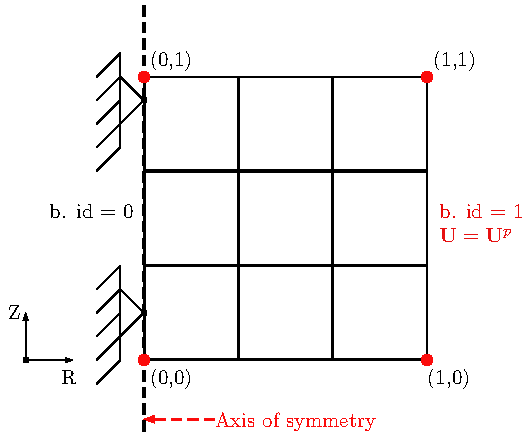
\includegraphics[width=0.95\textwidth]{patch_test_grid.pdf}
\caption{Uniform grid}
\label{fig:2.1.1}
\end{subfigure}
\begin{subfigure}{0.4\textwidth}
\centering
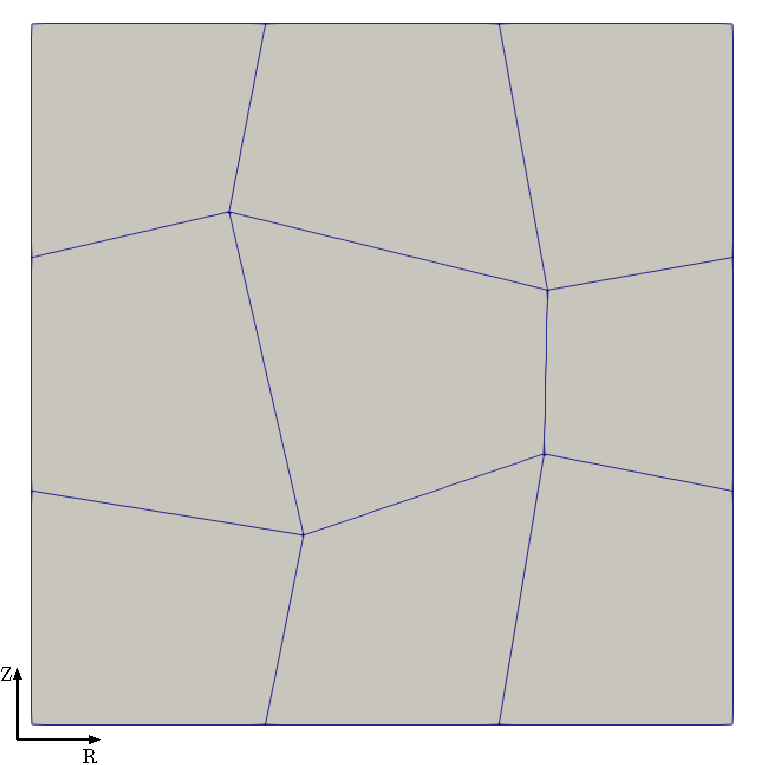
\includegraphics[width=0.8\textwidth]{patch_distort_grid.pdf}
\caption{Distorted grid}
\label{fig:2.1.2}
\end{subfigure}
\caption{Patch test unit cube geometry}
\label{fig:2.1}
\end{figure}

We consider an axisymmetric geometry with unit cube cross section which is discretized into nine elements, cf. \Cref{fig:2.1.1}. To check for the discretization error in the numerical solution using a selected finite element, we also have a distorted grid with the grid points in the interior of mesh distorted in a random way, cf. \Cref{fig:2.1.2}. The hyperelastic Neo-Hookean material model as given in \Cref{eq:2.2} was considered for the patch material. The material parameters chosen for this test were $\mu = 3e^{-2}$ Pa and $\nu = 0.4$. The considered boundary conditions are: homogeneous Dirichlet boundary condition on the boundary along the axis of symmetry (boundary id = 0) and inhomogeneous Dirichlet boundary condition (tensile load) on boundary id = 1. The prescribed displacement of $0.1 $m was applied in a uniformly increasing step of $0.025 $m. Lagrange finite elements with bi-linear and bi-quadratic shape functions were employed for this patch test. One h-adaptive mesh refinement cycle was performed to compare the quality of solution between the coarse mesh and once h-adaptively refined mesh for the distorted grid geometry. \par 

\begin{figure}[h]
\centering
\begin{subfigure}[b]{0.35\textwidth}
\centering
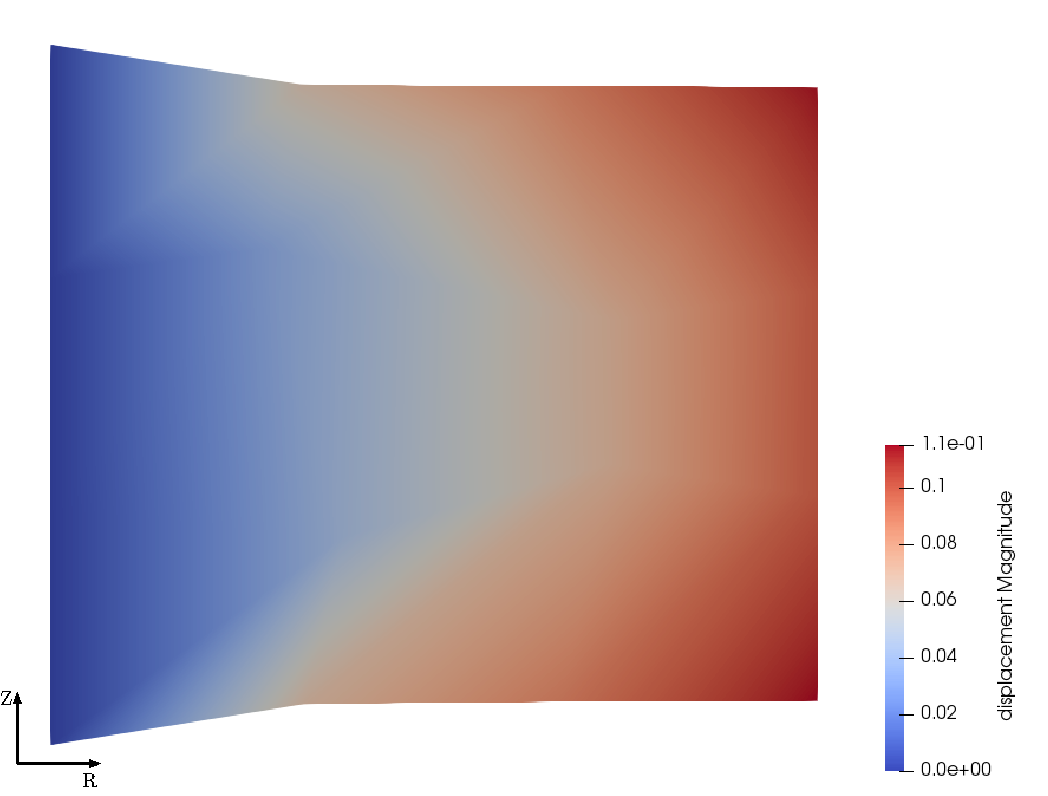
\includegraphics[width=0.9\textwidth]{patch_distort_grid_ref_0.pdf}
\caption{Linear element: Ref. cycle 0}
\label{fig:2.2.1}
\end{subfigure}
\begin{subfigure}[b]{0.35\textwidth}
\centering
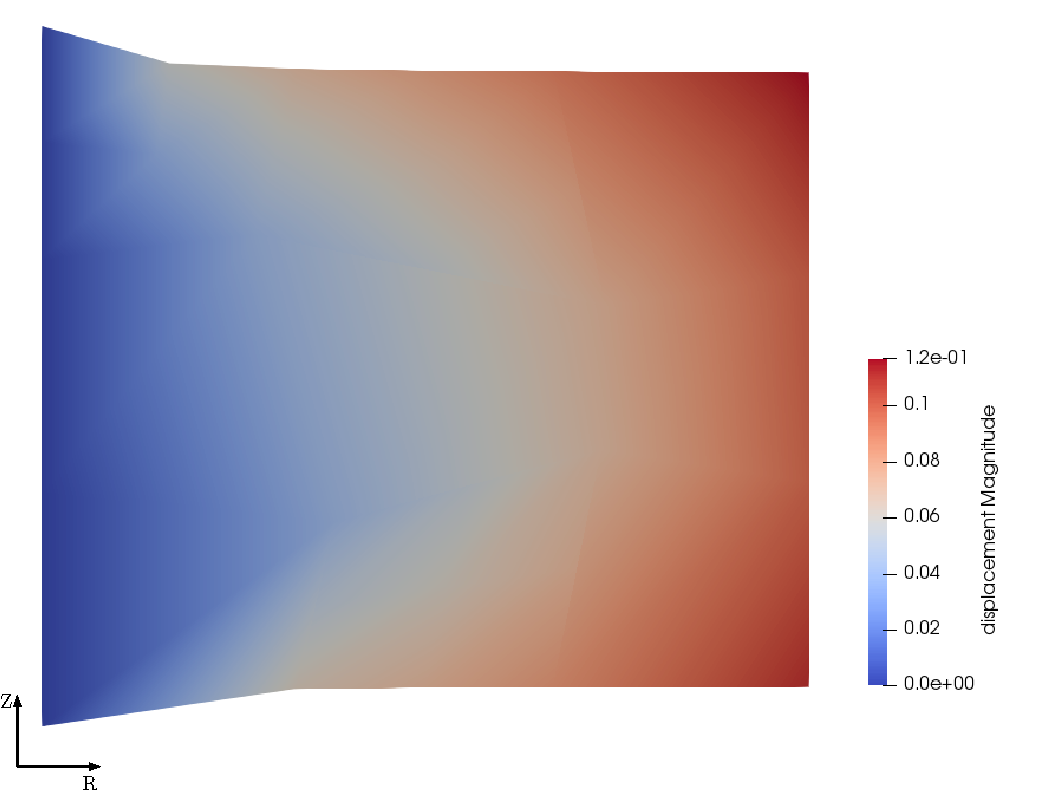
\includegraphics[width=0.9\textwidth]{patch_distort_grid_ref_1.pdf}
\caption{Linear element: Ref. cycle 1}
\label{fig:2.2.2}
\end{subfigure}
\begin{subfigure}[b]{0.35\textwidth}
\centering
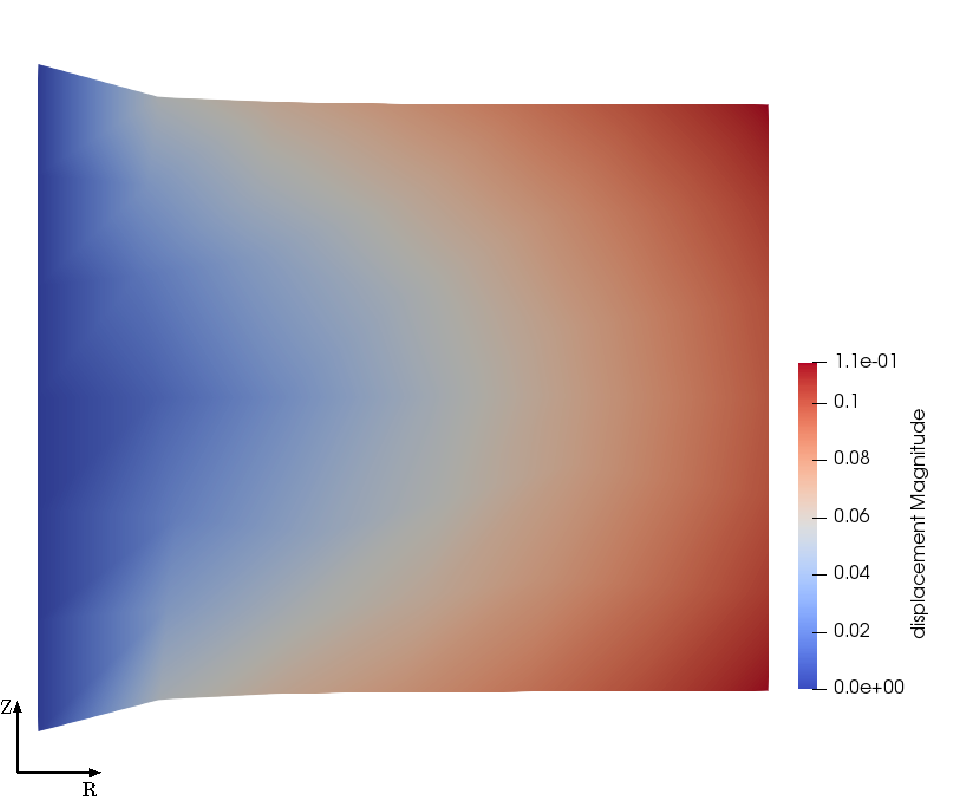
\includegraphics[width=0.9\textwidth]{patch_distort_grid_ref_0_quad.pdf}
\caption{Quadratic element: Ref. cycle 0}
\label{fig:2.2.3}
\end{subfigure}
\begin{subfigure}[b]{0.35\textwidth}
\centering
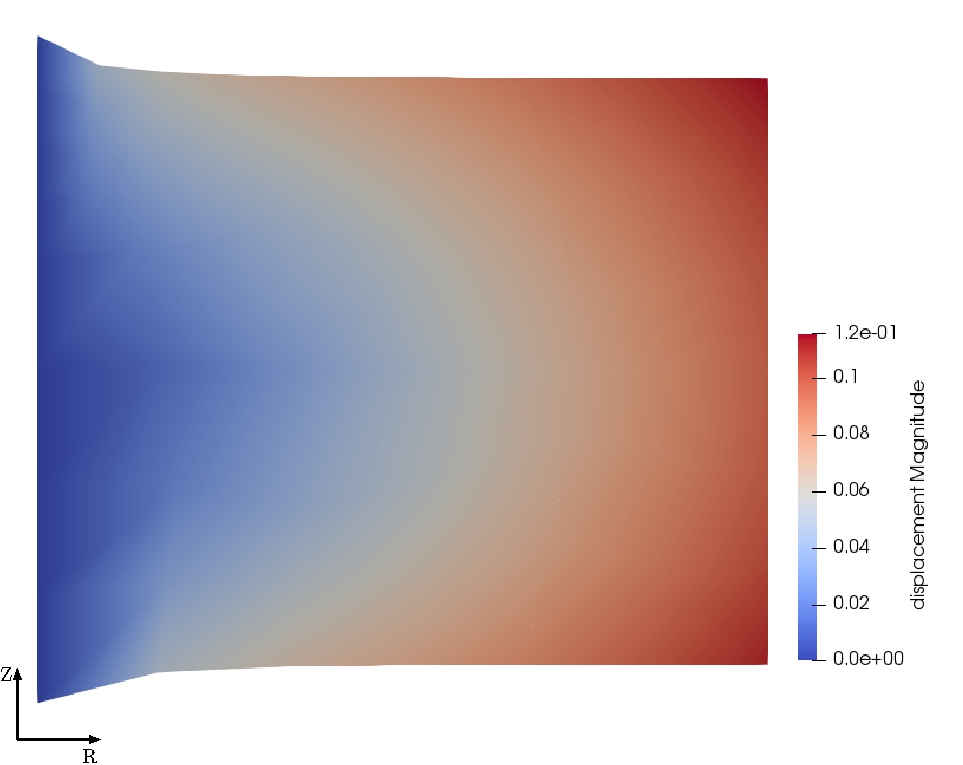
\includegraphics[width=0.9\textwidth]{patch_distort_grid_ref_1_quad.pdf}
\caption{Quadratic element: Ref. cycle 1}
\label{fig:2.2.4}
\end{subfigure}
\caption{Distorted grid displacement at total load}
\label{fig:2.2}
\end{figure}

\begin{figure}[h!]
\centering
\begin{subfigure}[b]{0.35\textwidth}
\centering
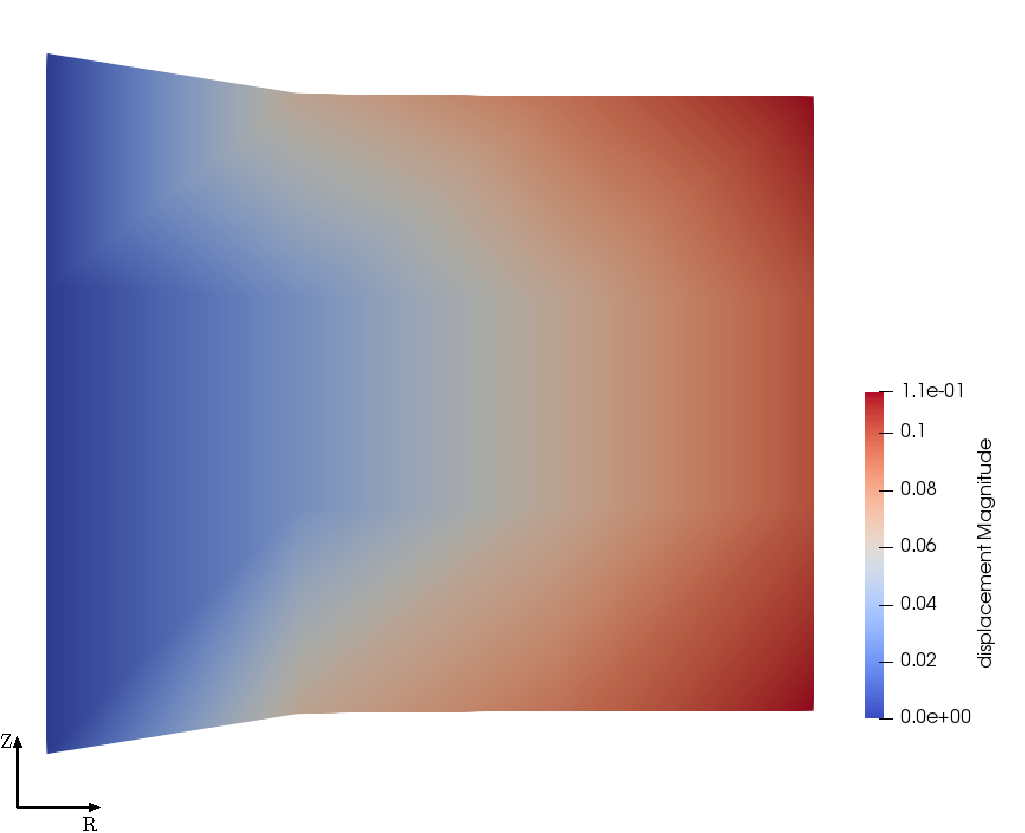
\includegraphics[width=0.9\textwidth]{patch_uniform_grid_ref_0.pdf}
\caption{Linear element: Ref. cycle 0}
\label{fig:2.3.1}
\end{subfigure}
\begin{subfigure}[b]{0.35\textwidth}
\centering
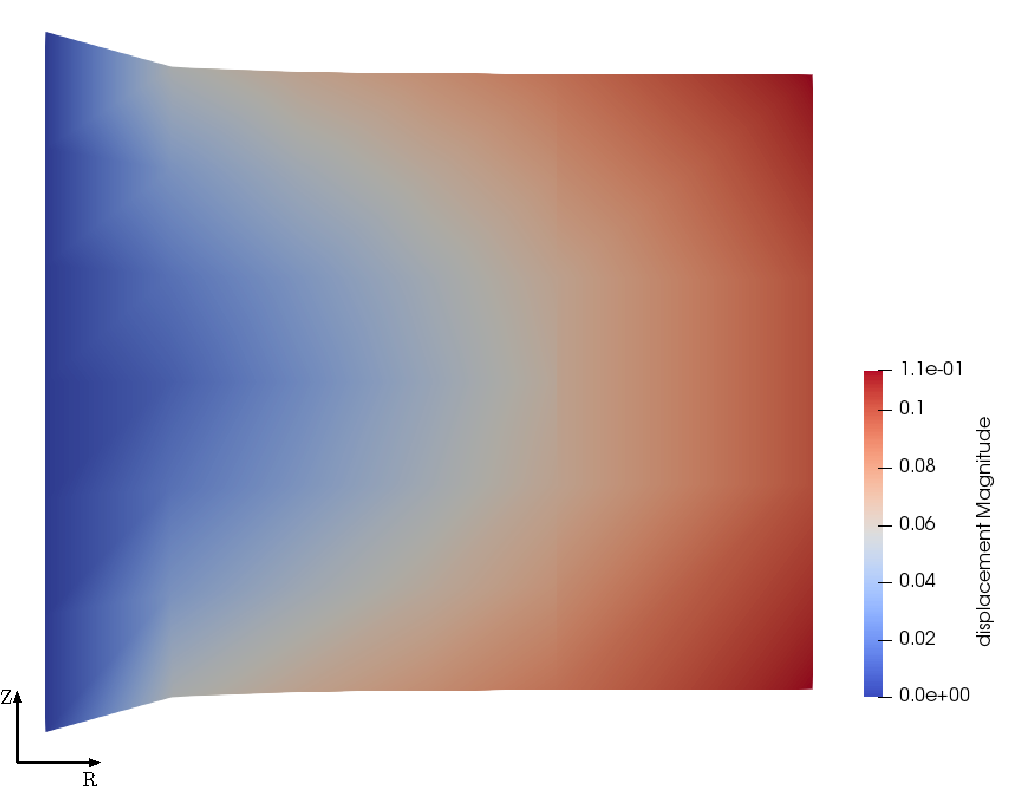
\includegraphics[width=0.9\textwidth]{patch_uniform_grid_ref_1.pdf}
\caption{Linear element: Ref. cycle 1}
\label{fig:2.3.2}
\end{subfigure}
\begin{subfigure}[b]{0.35\textwidth}
\centering
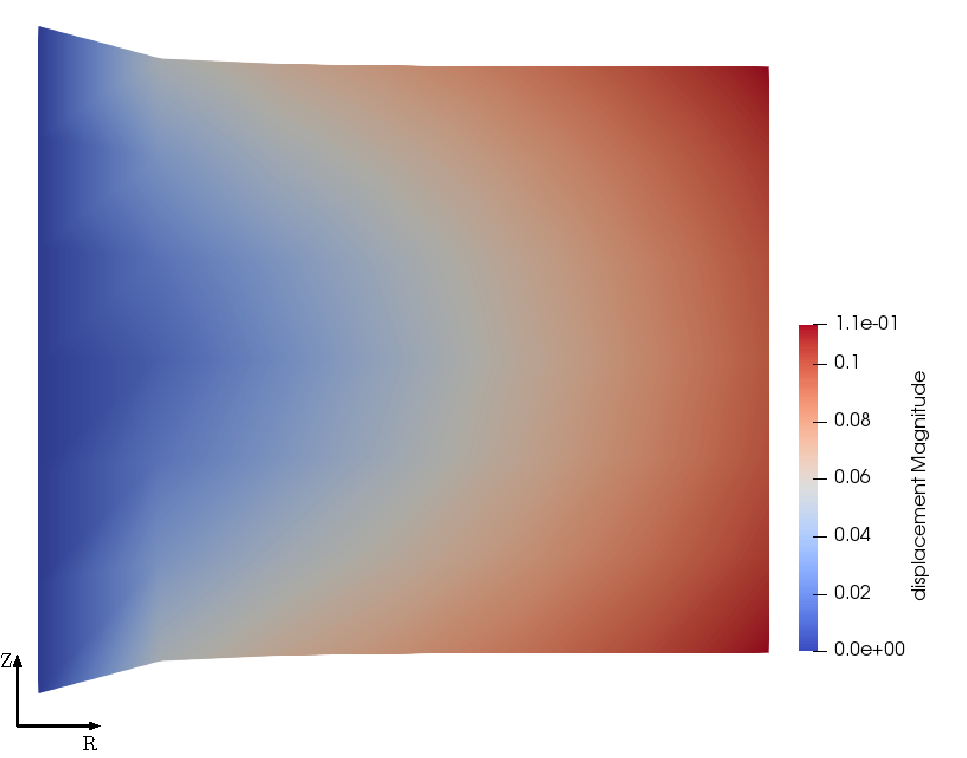
\includegraphics[width=0.9\textwidth]{patch_uniform_grid_ref_0_quad.pdf}
\caption{Quadratic element: Ref. cycle 0}
\label{fig:2.3.3}
\end{subfigure}
\begin{subfigure}[b]{0.35\textwidth}
\centering
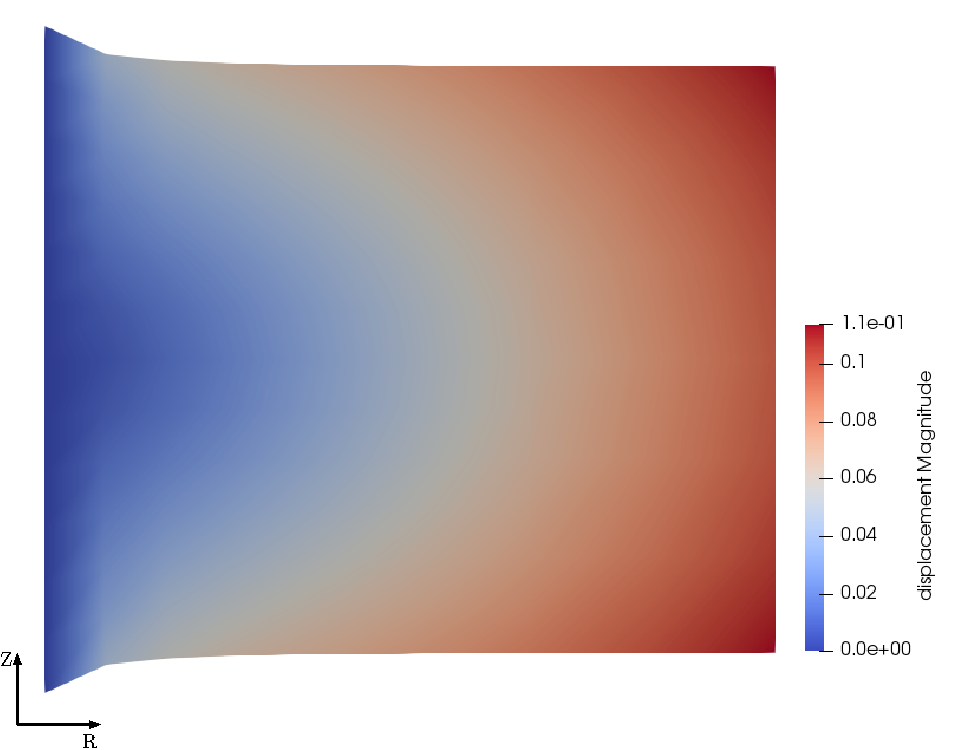
\includegraphics[width=0.9\textwidth]{patch_uniform_grid_ref_1_quad.pdf}
\caption{Quadratic element: Ref. cycle 1}
\label{fig:2.3.4}
\end{subfigure}
\caption{Uniform grid displacement at total load}
\label{fig:2.3}
\end{figure}

Comparing the results for the final deformed states for the distorted mesh in \Cref{fig:2.2} and the uniform grid patch in \Cref{fig:2.3}, we can confirm that the employed bi-linear (vector-valued) shape functions $(Q_1 \times Q_1)$ for the displacement field lead to qualitatively similar results (under given tolerance) as the ones for the bi-quadratic shape functions $(Q_2 \times Q_2)$. In the regions with high solution gradient (here the cells near the boundary with boundary id $= 0$), an increase in the number of degrees of freedom due to h-adaptive mesh refinement would lead to a higher accuracy solution. Thus, the deformed states after one refinement cycle for the distorted grid are different compared to the uniform grid results. But the nature of the displacement field is similar irrespective of the employed bi-linear or bi-quadratic shape functions. \par 

\subsubsection{Traction boundary condition test}
A unit test to check the traction boundary condition implementation was set up with an axisymmetric beam geometry problem. The considered beam is of length $2$ m and height $1$ m. The beam is discretized into 8 elements along the length and 4 elements along the height, thus giving a total of 32 elements in the coarse mesh. The hyperelastic Neo-Hookean material model as given in \Cref{eq:2.2} was considered for the beam material. The chosen material parameters for this test were $\mu = 3e^{-2}$ Pa and $\nu = 0.4$. The considered boundary conditions are: homogeneous Dirichlet boundary condition on the boundary along the axis of symmetry with boundary id = 0 and a uniformly distributed traction load (-Z) on the right half of the top boundary of the beam with boundary id = 6, cf. \Cref{fig:2.4}. The considered traction load has a magnitude of $1e^{-3} \frac{\text{N}}{\text{m}}$ distributed uniformly over a length of $1 \ \text{m}$. Employing uniformly increasing load stepping, this traction load was applied in four load steps. \par    

\begin{figure}[h]
\centering 
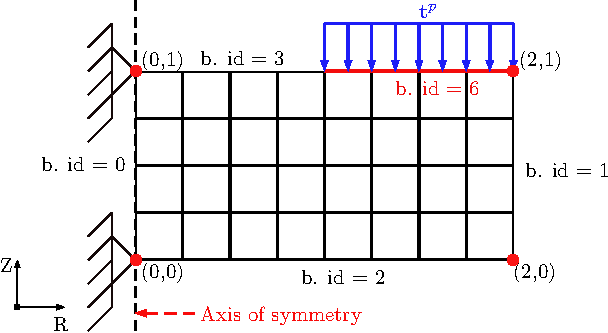
\includegraphics[width=0.5\textwidth]{beam_grid.pdf}
\caption{Beam problem with traction load}
\label{fig:2.4}
\end{figure} 

\begin{figure}[h]
\centering
%\begin{subfigure}[b]{0.45\textwidth}
%\centering
%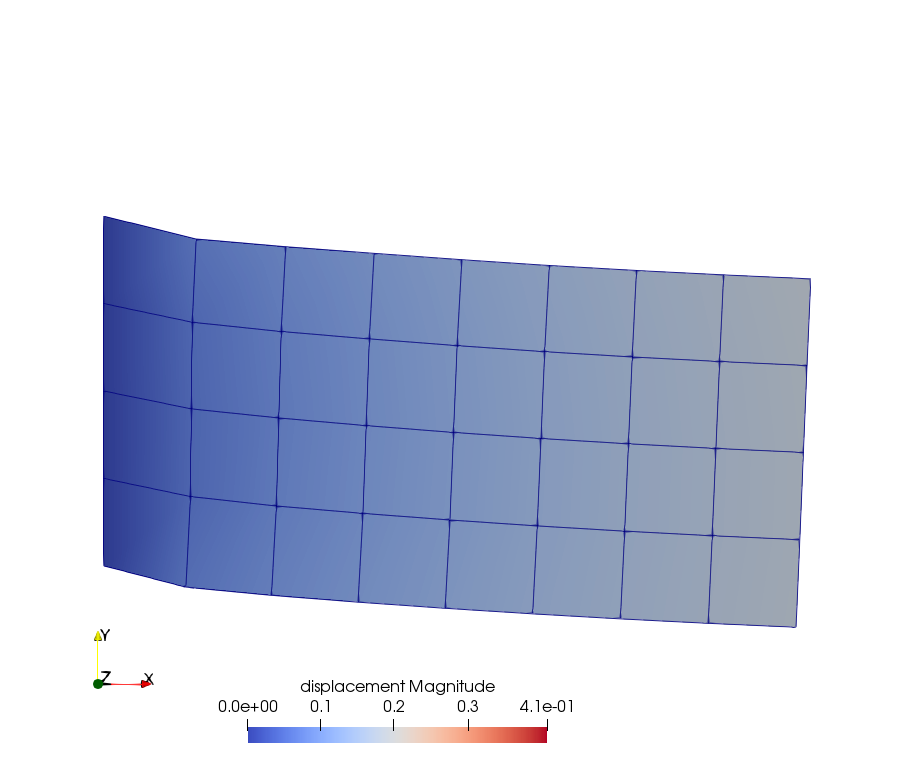
\includegraphics[width=0.9\textwidth]{beam_ref_0_load_half.png}
%\caption{Ref. cycle 0 (half load)}
%\label{fig:1.5.1}
%\end{subfigure}
\begin{subfigure}[b]{0.45\textwidth}
\centering
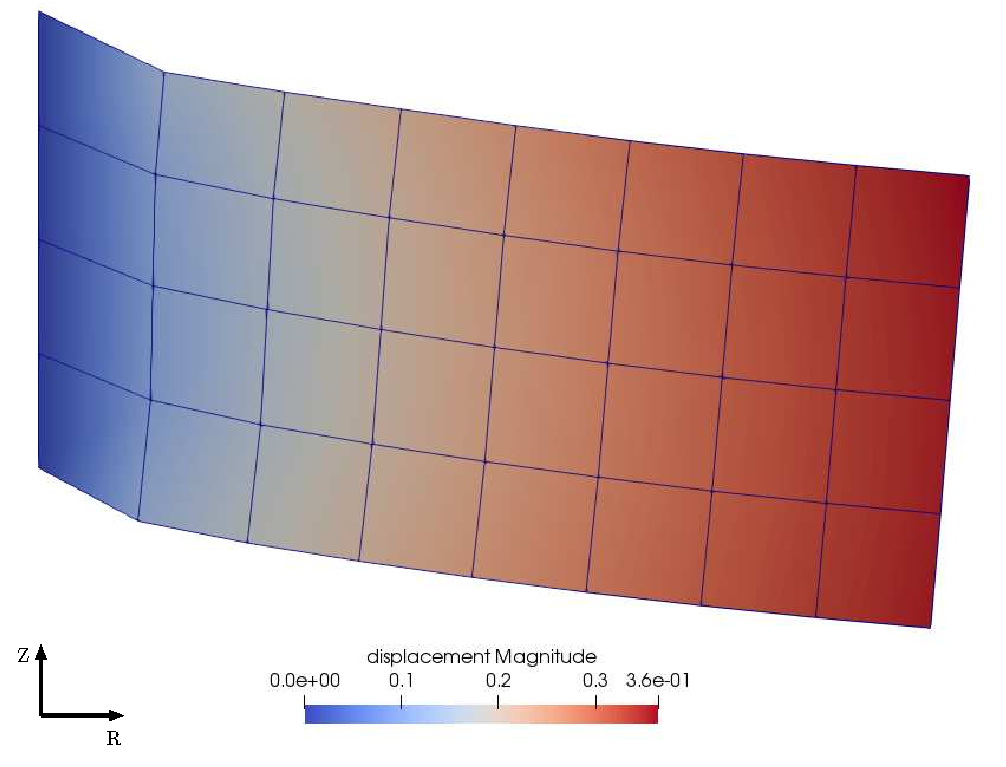
\includegraphics[width=0.9\textwidth]{beam_ref_0_full_load.pdf}
\caption{Ref. cycle 0}
\label{fig:2.5.2}
\end{subfigure}
%\begin{subfigure}[b]{0.45\textwidth}
%\centering
%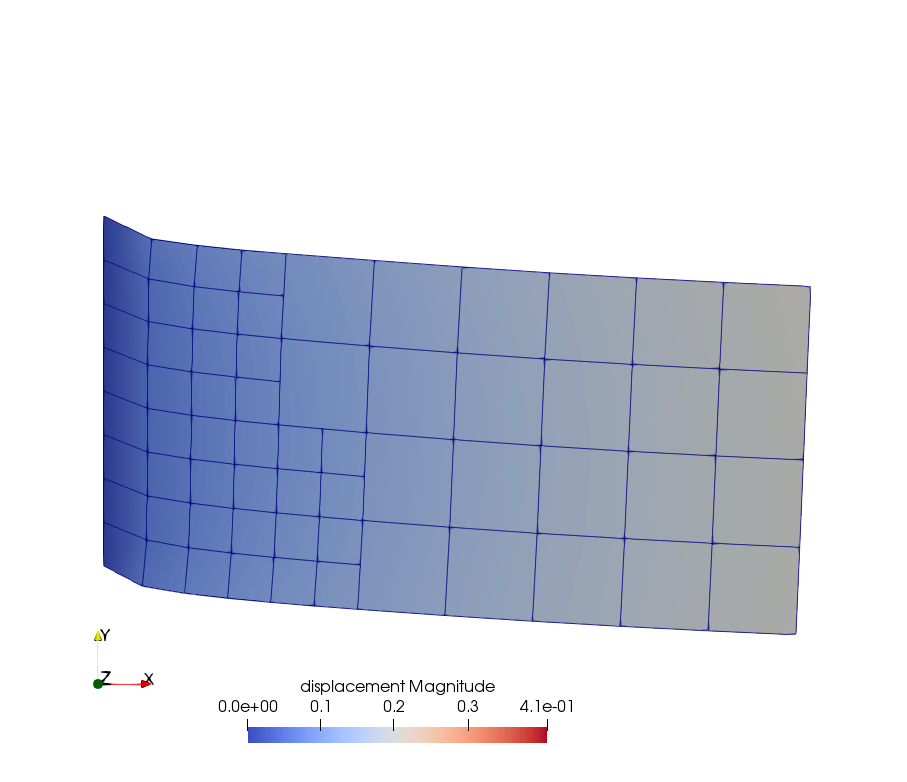
\includegraphics[width=0.9\textwidth]{beam_ref_1_load_half.png}
%\caption{Ref. cycle 1 (half load)}
%\label{fig:1.5.3}
%\end{subfigure}
\begin{subfigure}[b]{0.45\textwidth}
\centering
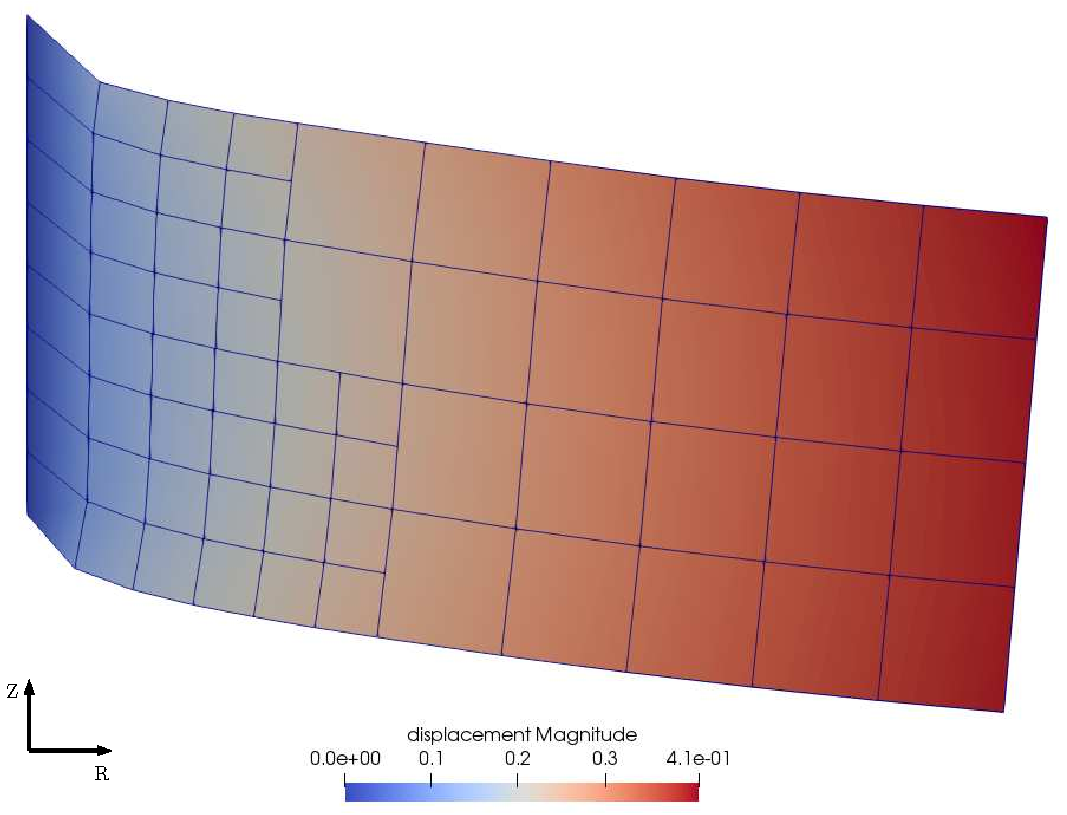
\includegraphics[width=0.9\textwidth]{beam_ref_1_full_load.pdf}
\caption{Ref. cycle 1}
\label{fig:2.5.4}
\end{subfigure}
\caption{Beam displacement}
\label{fig:2.5}
\end{figure}

In the following, the algorithmic scheme for h-adaptive mesh refinement is highlighted. Due to a high solution gradient in the elements near the axis of symmetry (b.id = 0) in the coarse grid, cf \Cref{fig:2.5.2}, the resulting error in solution is high in these elements. To reduce the error in the solution we need to make the mesh fine where the local ($H^2$) norm of the solution is large. We compute a local indicator of error $\eta_K$ for every cell K employing a standard error estimator such as the ``\textbf{Kelly error estimator}'' from the literature \cite{Kelly1983} which constitutes to an ``\textbf{a-posteriori}'' error estimate. The local Kelly error indicator $\eta_K$ for each cell is given as 
\begin{equation}
\eta_K \coloneqq h_K^{\frac{1}{2}} \left( \ \int\limits_{\partial K} \seminorm{{\llbracket\nabla \mathbf{u_h} \rrbracket}}^2 \ \right)^{\frac{1}{2}},
\label{eq:2.27}
\end{equation}
where $h_k$ is taken to be the greatest length of the diagonals of the cell K, $\nabla \mathbf{u_h}$ is the gradient of the computed FE solution and $\llbracket\nabla \mathbf{u_h} \rrbracket$ denotes the jump in the gradient which is an indicator of the second derivative of the solution field. \par 

\Cref{alg:2.2} highlights the procedure one carries out to perform h-adaptive mesh refinement. We employ the \textbf{SOLVE-ESTIMATE-MARK-REFINE} cycle for adaptive refinement. In the solve phase we assemble the linear system of equations and solve it on the coarse/current mesh. By use of heuristically derived error estimator such as the Kelly error estimator, we estimate the error on each cell of the mesh. In the mark phase, following some chosen strategy we mark the cells with largest error for refinement and coarsening. In the last phase, we refine and coarsen the marked cells and continue this iterative procedure for a user selected number of refinement cycles. More details of the refinement procedure with the mathematical foundations for the error estimator and the different marking strategies one can employ can be found in \cite[Chapter 4]{Gholap_project}. \par 

\begin{algorithm}[h]
\begin{enumerate}
\item Start with the coarse mesh
\item Solve on this mesh
\item Compute error indicator $\eta_K$ for every cell based on the numerical solution
\item Mark a fraction of the cells with largest error
\item Refine the marked cells to get the new mesh
\item Start over at 2
\end{enumerate}
\caption{\textbf{H-ADAPTIVE MESH REFINEMENT CYCLE}}
\label{alg:2.2} 
\end{algorithm}

The final deformed state for individual refinement cycles are as observed in \Cref{fig:2.5.2} and \Cref{fig:2.5.4}. As expected, upon mesh refinement we observe the solution field is more accurate and has reduced jump in the gradient of the solution field in the (refined) cells near the axis of symmetry. This test proves the effectiveness of an adaptively refined mesh in computing the solution more accurately and motivates the need of such adaptivity in the region of interest for a complex geometry and multi-physics problem discussed in the further section.\par  

\subsubsection{Test for instability behaviour}

Mechanical instability is an important phenomenon in determining the limit loads a structure can handle before becoming unstable. A stable design of the structure exists when the deformations increase as the applied load increases; an unstable design occurs when the deformations increase as the load decreases due to loss of stiffness. The study of such finite elastic deformations of structures helps in understanding the limit loads and prevent sudden buckling/snap-through failures of the structure for applied loads. Referring to \Cref{fig:2.8} commonly known as the load-deflection plot of the equilibrium path, elastic limit point is the critical point after which the structure/material begins to deform largely even for slightly increasing loads. For a load past the critical limit point $(1)$, the structure undergoes a non-linear buckling which includes a post-buckling instability region. The ``snap-through'' occurs in the non-linear instability region and the equilibrium path goes from one stable point $(1)$ to another stable point $(2)$. The non-linear behaviour places the next stable point $(2)$ at the same critical limit load as point $(1)$, but this new load limit at point $(2)$ now corresponds to a new structural shape \cite{Hrinda2010}. The slope of the equilibrium path during the snap-through eventually becomes zero. The slope of this curve is also known as ``tangent stiffness''. From a mathematical point of view the determination of instability points is related to the investigation of tangent stiffness with respect to singularities. At the bifurcation point a secondary equilibrium path branches off the primary equilibrium path. Bifurcation point is the limit point at which the structure immediately becomes unstable and buckles. The structure is unable to support any further loads. \par 

\begin{figure}[h]
\centering 
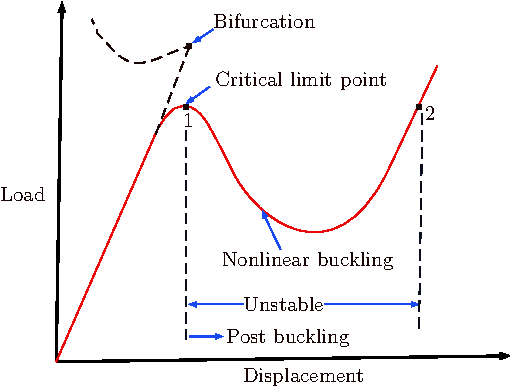
\includegraphics[width=0.6\textwidth]{nonlinear_eq_path.pdf}
\caption{Equilibrium paths for non-linear buckling}
\label{fig:2.8}
\end{figure}

\begin{figure}[ht!]
\centering
\begin{subfigure}[b]{0.7\textwidth}
\centering
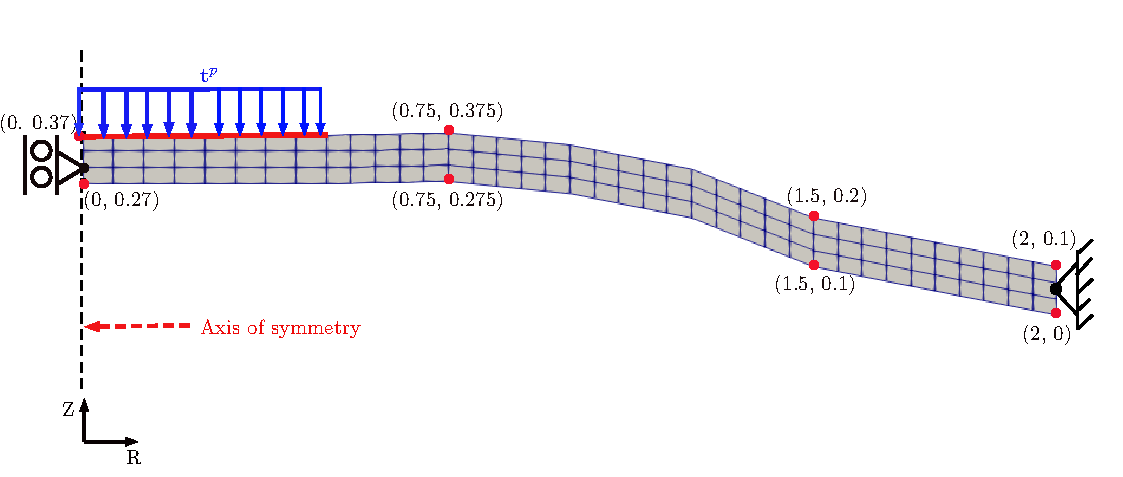
\includegraphics[width=0.95\textwidth]{hooped_beam_grid.pdf}
\caption{Hooped beam test model}
\label{fig:2.6.1}
\end{subfigure}
\begin{subfigure}[b]{0.29\textwidth}
\centering
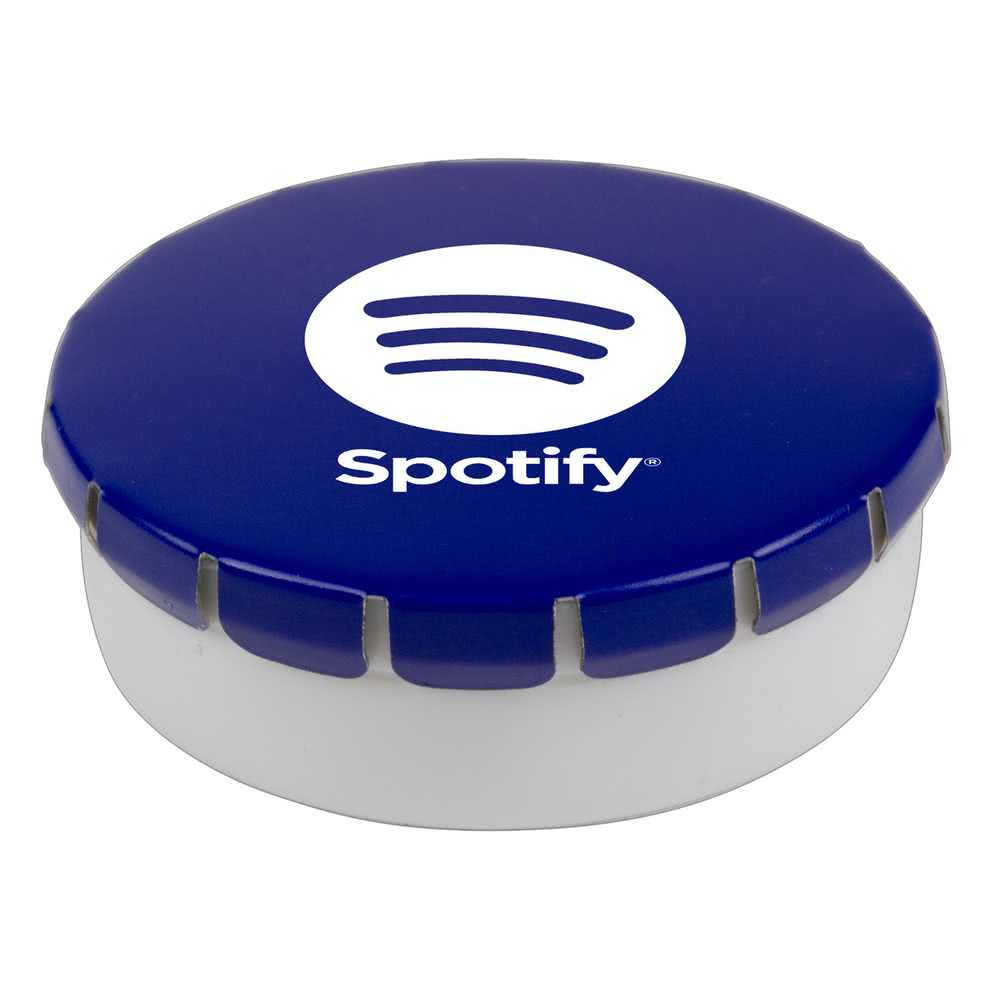
\includegraphics[width=0.8\textwidth]{snap_top_mint_box.jpg}
\caption{Mint box that exhibits snap through behaviour}
\label{fig:2.6.2}
\end{subfigure}
\caption{Mechanical instability test model 1}
\label{fig:2.6}
\end{figure}

For the stability analysis two test models were implemented as seen in \Cref{fig:2.6.1} and \Cref{fig:2.14}. The first mechanical test model was inspired by a commonly occurring tin mint box with round top, \Cref{fig:2.6.2}, that snaps through to open the box. The cap of this box undergoes a sudden large deformation for an applied point load at the middle point of the round cap. This instability mode is a desired deformation to open the box. On application of equal loads on the opposite ends of the cap, the cap snaps back to the original shape/form to close the box. To simulate such a sudden snap through behaviour using robust non-linear solvers we developed the axisymmetric hooped beam test model as illustrated in \Cref{fig:2.6.1}. The out-of-plane displacement of the beam end is fixed by considering pin support (homogeneous Dirichlet boundary condition) and the edge lying on the axis of symmetry has a ``sliding'' constraint ($u_x = 0, u_y \neq 0$) that preserves the symmetry about the axis of the problem. A uniformly distributed traction load $\mathbf{t}^p = 1.5e^{-4} \ \frac{\text{N}}{\text{m}}$ acts on the top surface of beam as shown in the model. The hyperelastic Neo-Hookean material model as stated in \Cref{eq:2.2} was considered for the hooped beam with material parameters $\mu = 3e^{-2}$ Pa and $\nu = 0.4$.\par 

\begin{figure}[ht!]
\centering
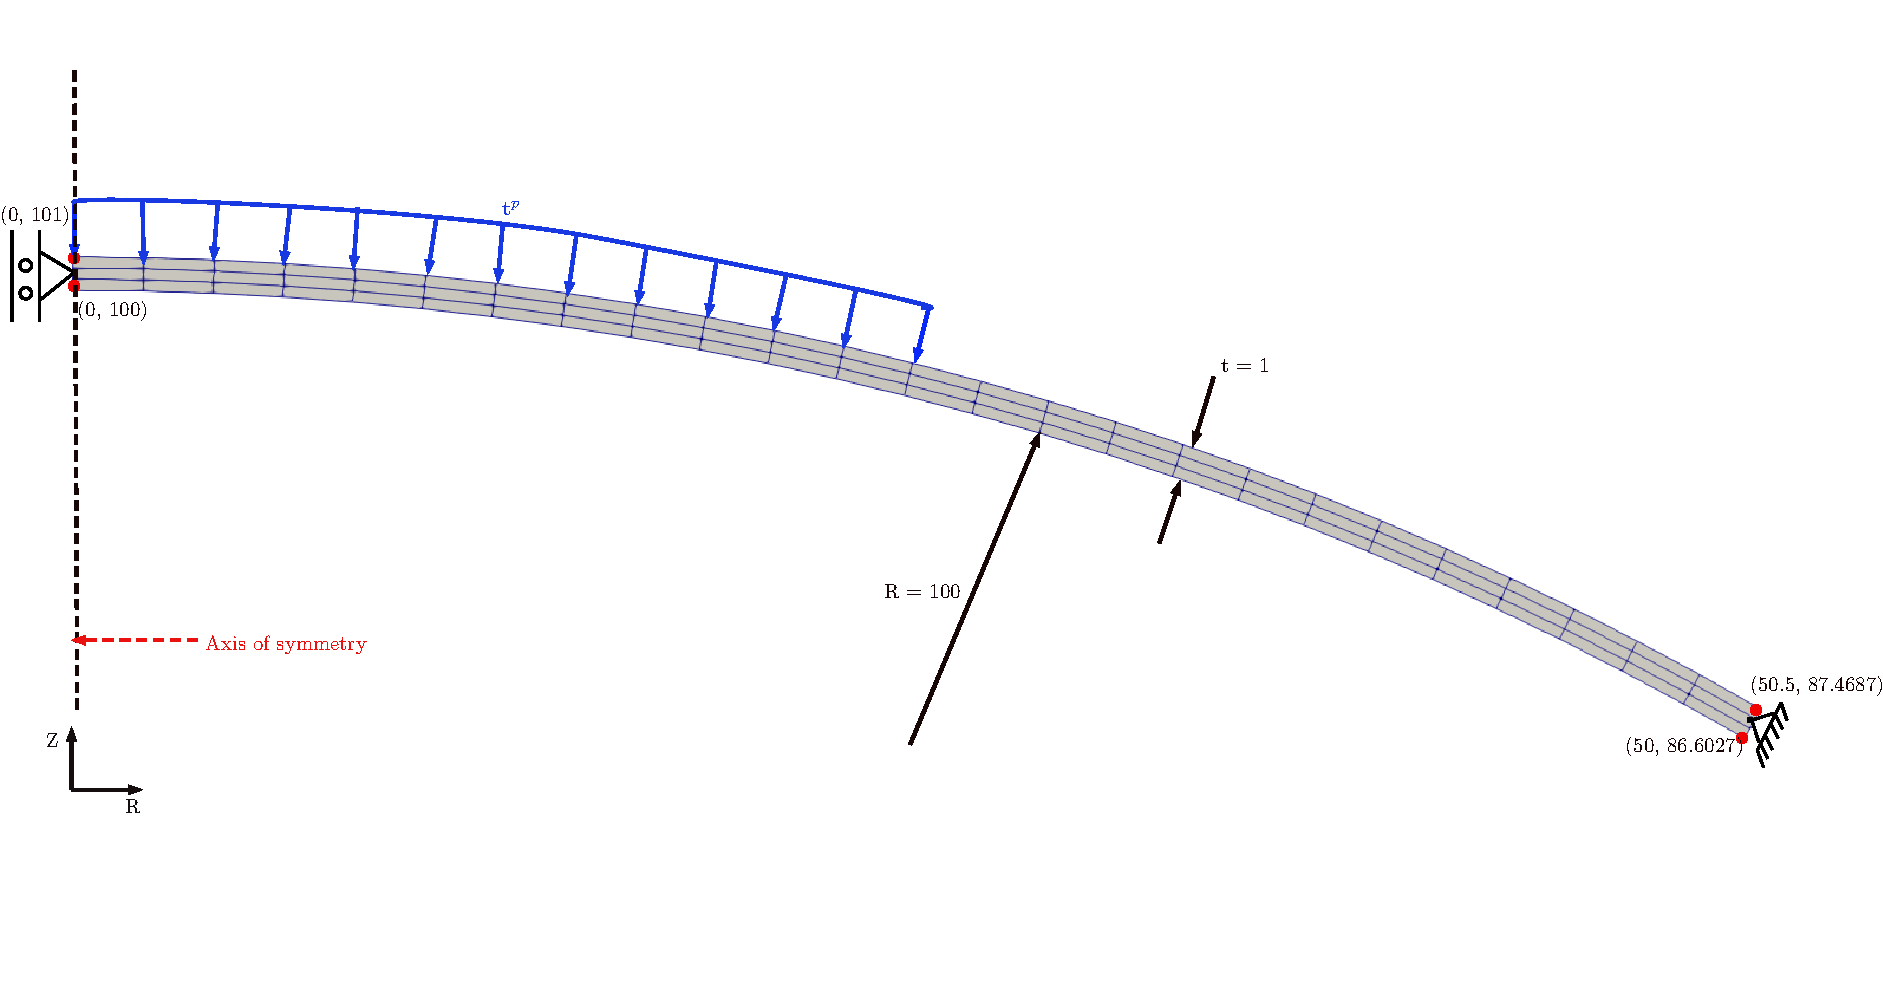
\includegraphics[width=0.8\textwidth]{crisfield_beam.pdf}
\caption{Crisfield beam test model}
\label{fig:2.14}
\end{figure}

The second test model to perform stability analysis of structures is the Crisfield beam, cf. \Cref{fig:2.14}, which is used as a standard benchmark test model to study instability modes \cite[see][page 170]{Wriggers2008} and \cite{Hrinda2010}. The considered beam has an inner radius of 100 m and outer radius of 101 m and the included angle of $\ang{30}$. For this test model, same boundary conditions were considered as used for the hooped beam test model. A uniformly distributed traction load $\mathbf{t}^p = 2e^{-4} \ \frac{\text{N}}{\text{m}}$ was applied as illustrated in the representative figure. Same material parameter values were considered as employed in the hooped beam model. \par 

\begin{figure}[ht!]
\begin{subfigure}[t]{0.49\linewidth}
\centering
\resizebox{\linewidth}{!}{
\begin{tikzpicture}[spy using outlines={rectangle, magnification=2.5,connect spies}]
\begin{axis}[
xlabel = $\text{Displacement (L2 norm)}$,
ylabel = $\text{Load}$,
%grid =both,
%grid style=dashed,
%minor grid style ={gray!30},
%major grid style ={gray!30},
%width=0.8\linewidth,
legend pos=north west,
]
\addplot[
color=red,
mark=x,
mark size=2pt,
line width=1pt,
]
table[x=Disp_norm,y=Load_value]{hooped_beam_eq_path.dat};
\addlegendentry{Eq. path}
% for spy
\coordinate (spypoint) at (axis cs:0.44,1.0e-4);
\coordinate (spyviewer) at (axis cs:0.4,0.2e-4);
\spy[width=3cm, height=1cm] on (spypoint) in node [fill=white] at (spyviewer);
\end{axis}
\end{tikzpicture}
}
\caption{Hooped beam test}
\label{fig:2.16.1}
\end{subfigure}
\begin{subfigure}[t]{0.49\linewidth}
\centering
\resizebox{\linewidth}{!}{
\begin{tikzpicture}[spy using outlines={rectangle, magnification=2,connect spies}]
\begin{axis}[
xlabel = $\text{Displacement (L2 norm)}$,
ylabel = $\text{Load}$,
%grid =both,
%grid style=dashed,
%minor grid style ={gray!30},
%major grid style ={gray!30},
%width=0.8\linewidth,
legend pos=north west,
]
\addplot[
color=red,
mark=x,
mark size=2pt,
line width=1pt,
]
table[x=Disp_norm,y=Load_value]{crisfield_beam_eq_path.dat};
\addlegendentry{Eq. path}
% for spy
\coordinate (spypoint) at (axis cs:2.75,1.0e-5);
\coordinate (spyviewer) at (axis cs:4,1.5e-4);
\spy[width=4.5cm, height=1cm] on (spypoint) in node [fill=white] at (spyviewer);
\end{axis}
\end{tikzpicture}
}
\caption{Crisfield beam test}
\label{fig:2.16.2}
\end{subfigure}
\caption{Equilibrium paths for test models}
\label{fig:2.16}
\end{figure}

The results using the Newton-Raphson solution method for the solution of the non-linear test models are presented in \Cref{fig:2.15}. The resulting load-displacement plots, also known as the equilibrium path, for the point $(0, 0.27)$ in the hooped beam test and the point $(0, 100)$ in the crisfield beam test are depicted in \Cref{fig:2.16} (lower edge points on the boundary along the axis of symmetry). For the hooped beam test, as observed in \Cref{fig:2.16.1}, in the early stages of loading, for each load increment of size $7.5e^{-7}$ N there is a proportional increase in the resulting displacement. We observe a linear relation between the load and displacement in this stage which one can identify as the initial linear response of a hyperelastic material. After a certain load limit is reached, we observe for a small load increment a resulting large displacement identified by the jumps in the cross marked points in the zoomed view in \Cref{fig:2.16.1}. This is also clearly observable in the results of \Cref{fig:2.15.1}. Between the load step number 134 and 135 corresponding to the zoomed region of interest, the structure undergoes a sudden large deformation for a small increment in the applied load. A similar result is also observed for the crisfield beam test in the early stages of loading cycle. The large jump in the displacement from $\approx 1.3$ m to $\approx 4.3$ m for a small increment of load of size $1e^{-6}$ N in \Cref{fig:2.16.2} indicates that the structure has undergone unstable deformation. This significantly large displacement is clearly illustrated in \Cref{fig:2.15.2} between the load step 10 and 11. This work softening of the structure is due to the reduced material stiffness after reaching a certain limit load point that leads to material instability and buckling. \par 

\begin{figure}[ht!]
\centering
\begin{subfigure}[b]{0.49\textwidth}
\centering
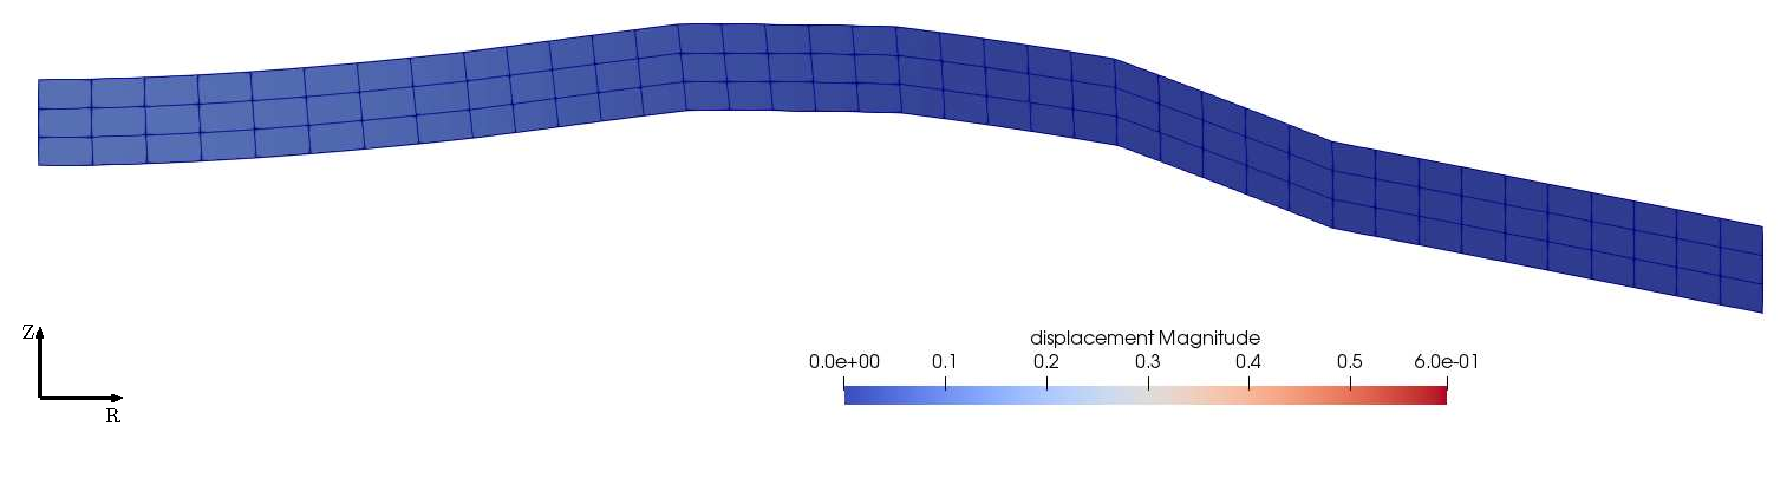
\includegraphics[width=0.95\textwidth]{hooped_beam_ls_50.pdf}
\caption*{Load step 50}
\vspace{1cm}
\centering
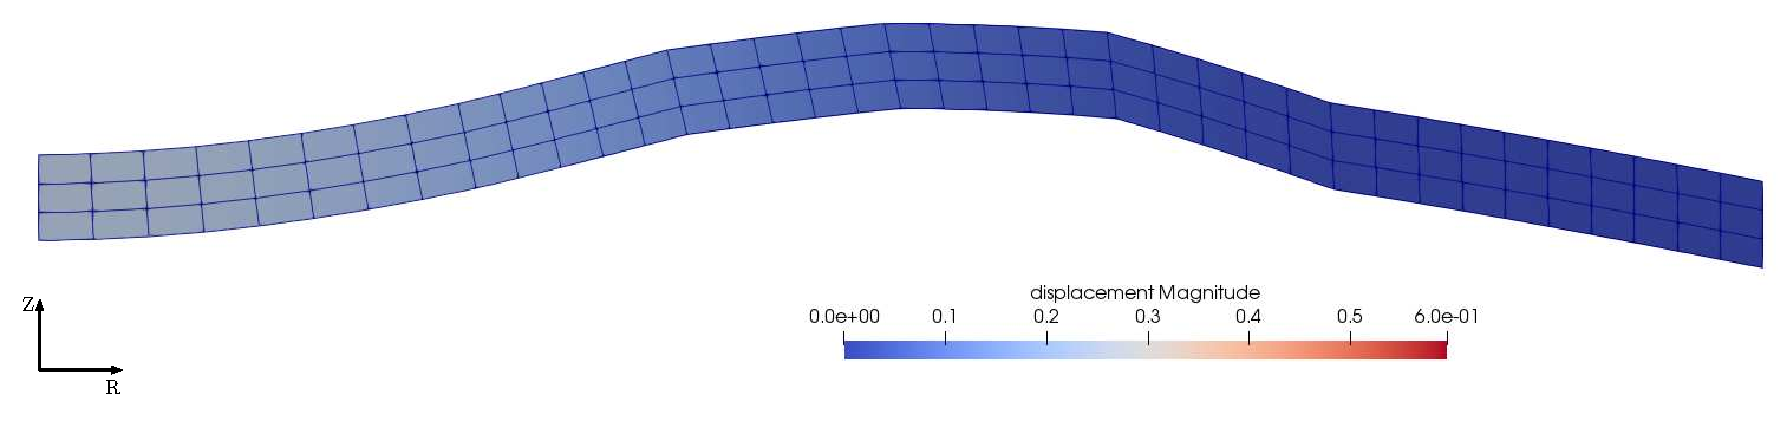
\includegraphics[width=0.95\textwidth]{hooped_beam_ls_100.pdf}
\caption*{Load step 100}
\vspace{1cm}
\centering
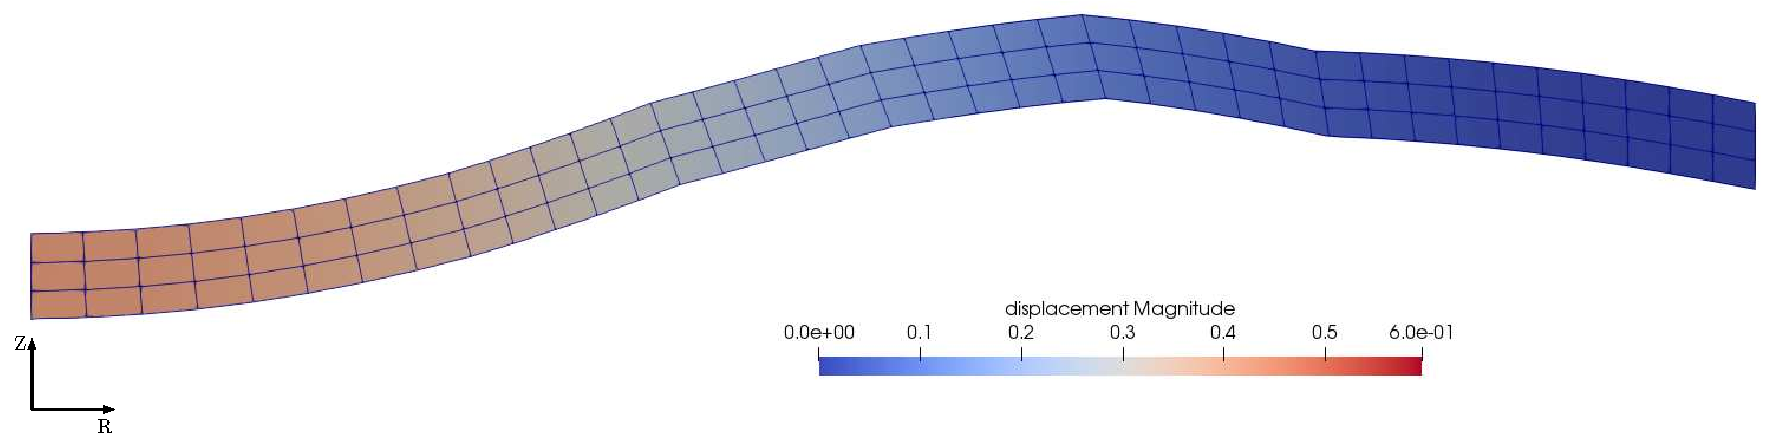
\includegraphics[width=0.95\textwidth]{hooped_beam_ls_134.pdf}
\caption*{Load step 134}
\vspace{1cm}
\centering
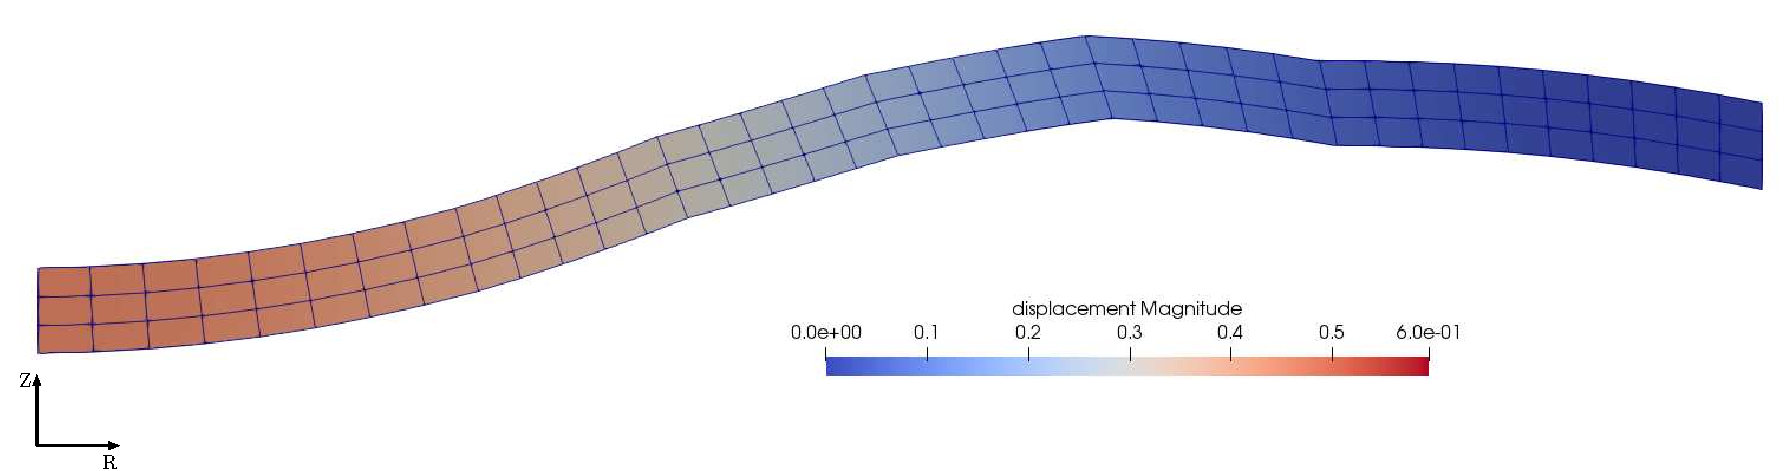
\includegraphics[width=0.95\textwidth]{hooped_beam_ls_135.pdf}
\caption*{Load step 135}
\vspace{1cm}
\centering
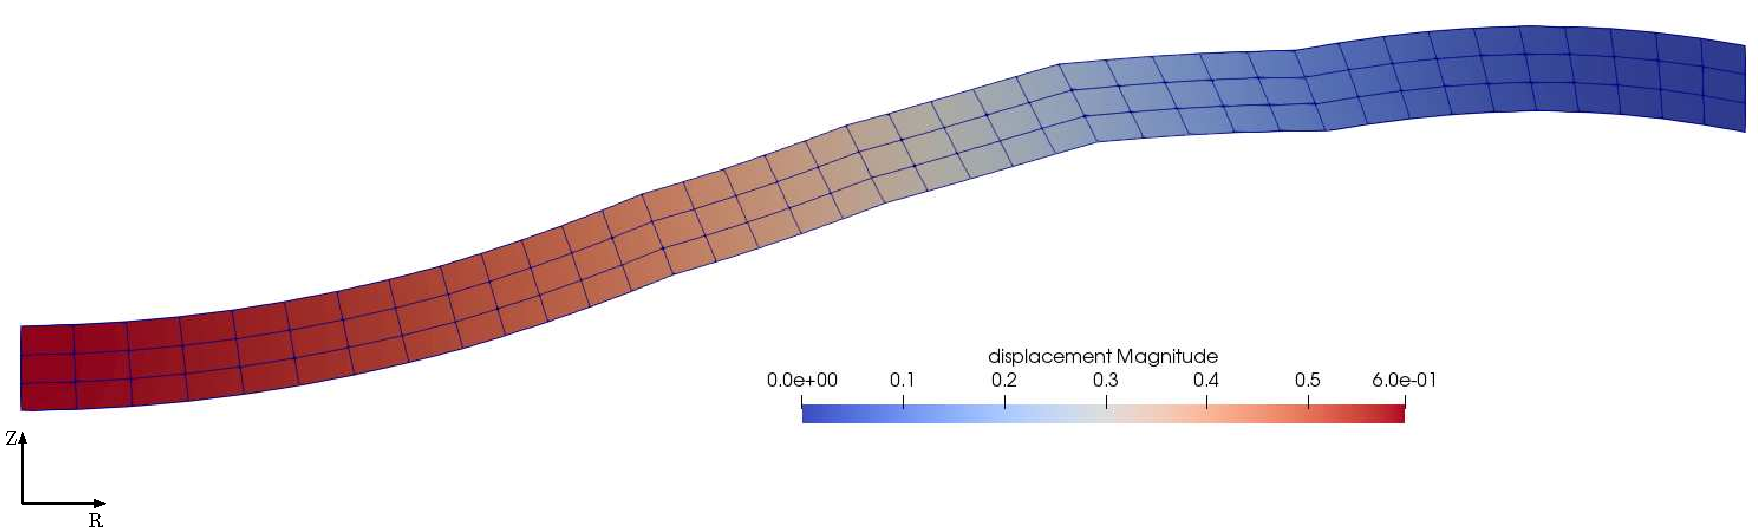
\includegraphics[width=0.95\textwidth]{hooped_beam_ls_199.pdf}
\caption*{Load step 199}
\caption{Hooped beam deformations}
\label{fig:2.15.1}
\end{subfigure}
\begin{subfigure}[b]{0.49\textwidth}
\centering
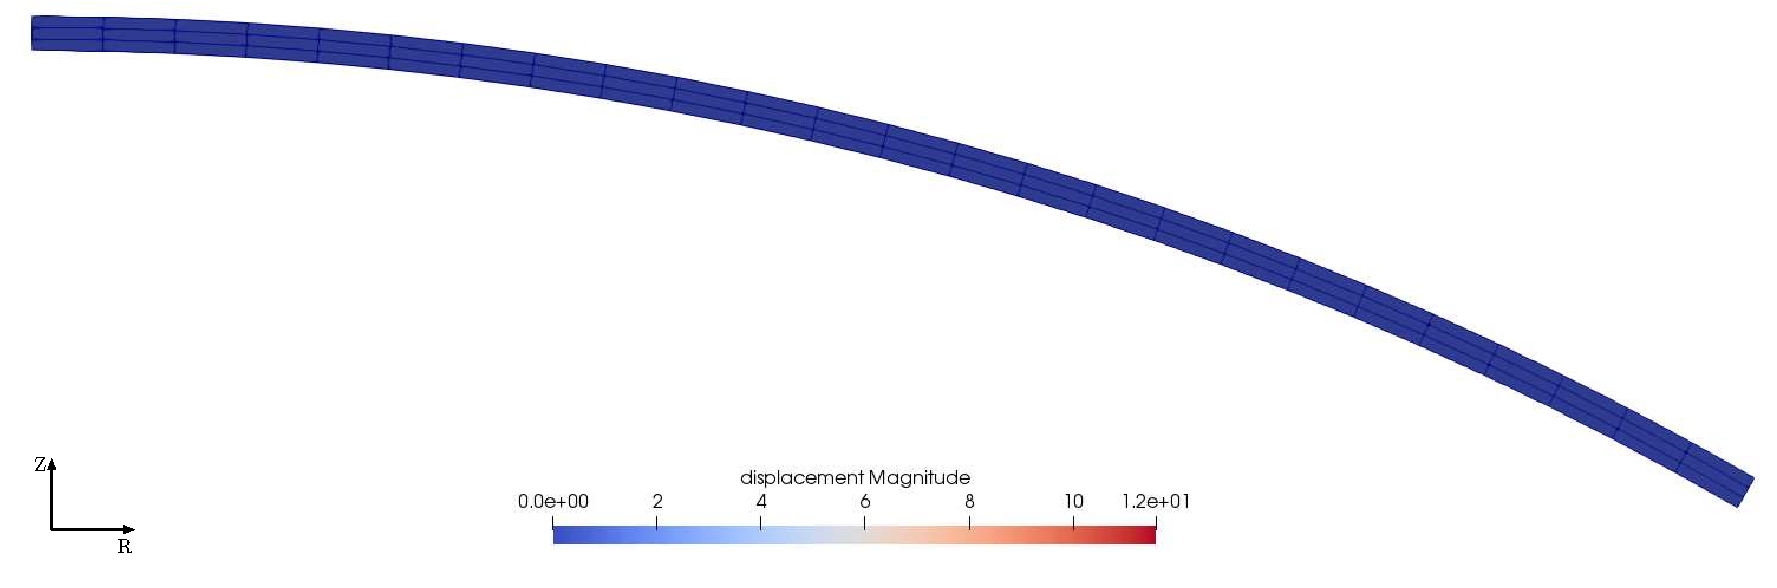
\includegraphics[width=0.95\textwidth]{crisfield_beam_ls_0.pdf}
\caption*{Load step 0}
\vspace{1cm}
\centering
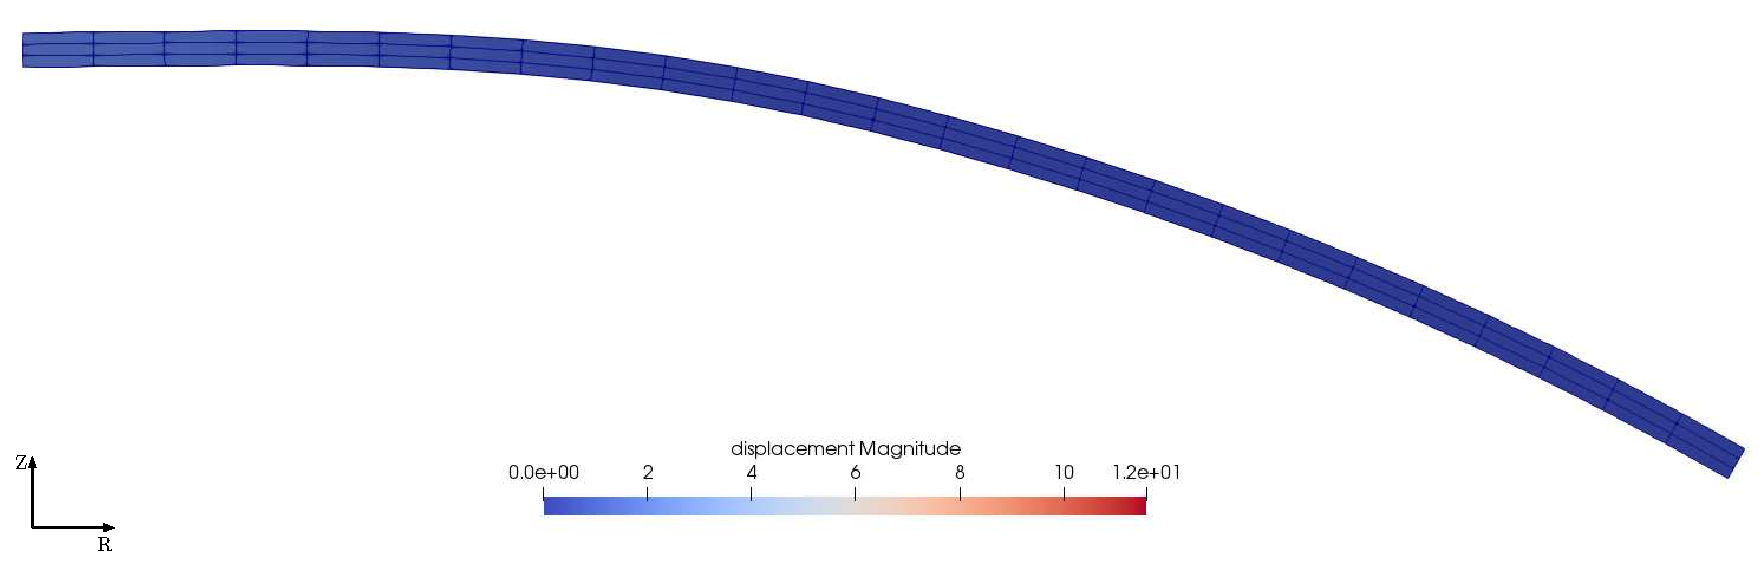
\includegraphics[width=0.95\textwidth]{crisfield_beam_ls_10.pdf}
\caption*{Load step 10}
\vspace{1cm}
\centering
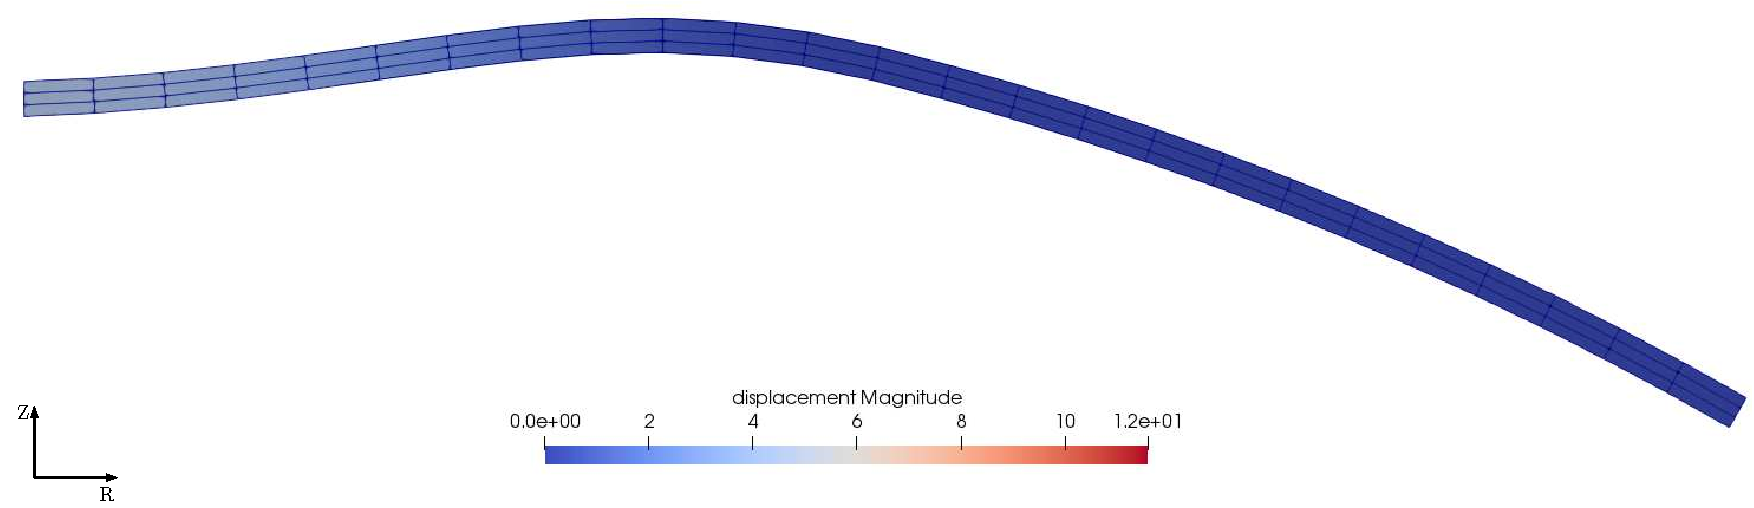
\includegraphics[width=0.95\textwidth]{crisfield_beam_ls_11.pdf}
\caption*{Load step 11}
\vspace{1cm}
\centering
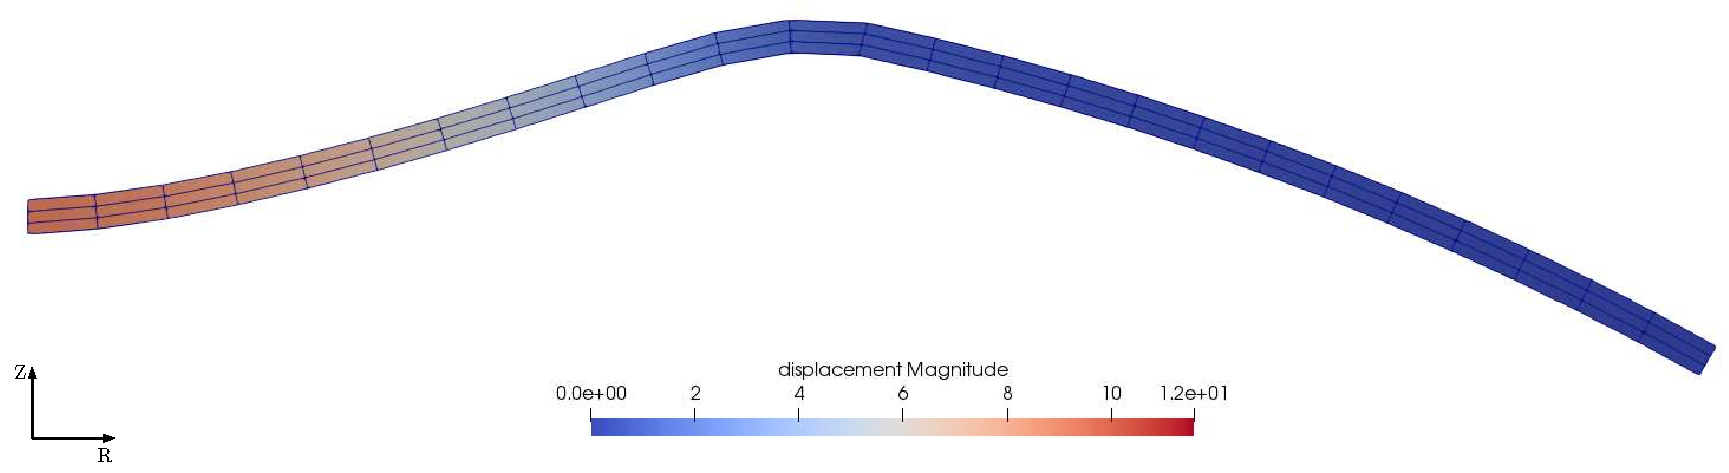
\includegraphics[width=0.95\textwidth]{crisfield_beam_ls_99.pdf}
\caption*{Load step 99}
\vspace{1cm}
\centering
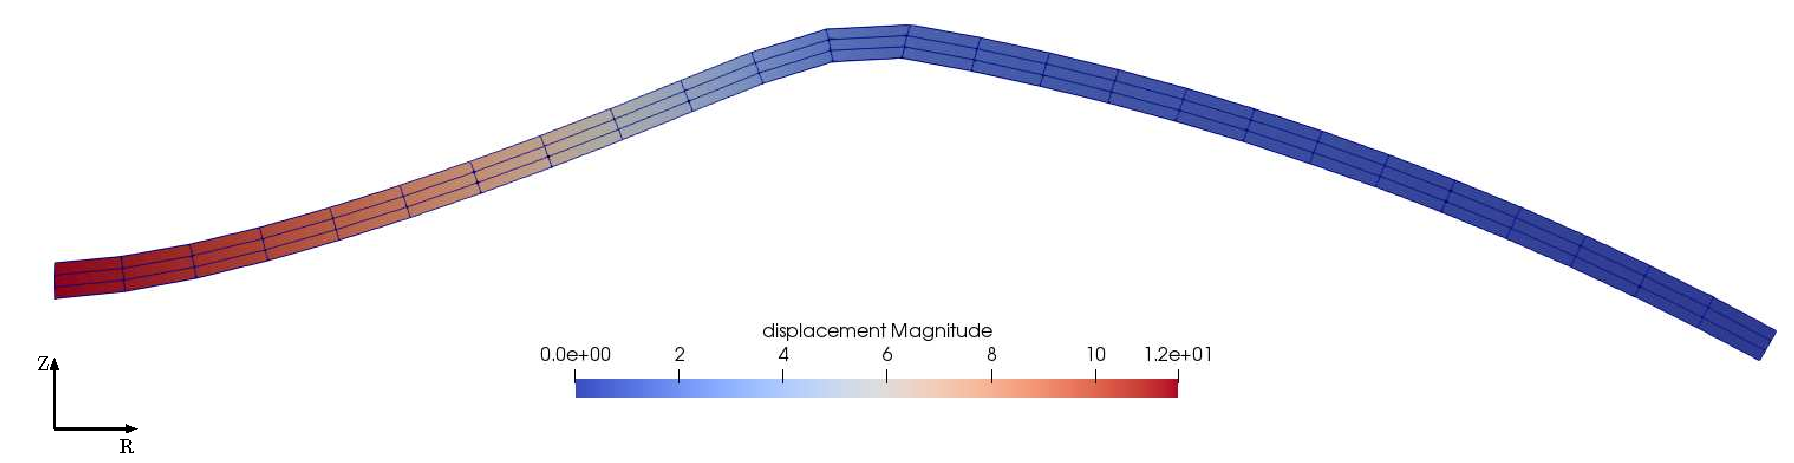
\includegraphics[width=0.95\textwidth]{crisfield_beam_ls_199.pdf}
\caption*{Load step 199}
\caption{Crisfield beam deformations}
\label{fig:2.15.2}
\end{subfigure}
\caption{Instability test results}
\label{fig:2.15}
\end{figure}

As observed in both the \Cref{fig:2.16.1,fig:2.16.2} in the region of interest near the limit point, the tangent to the equilibrium path, also known as the tangent stiffness, approaches to zero. As already pointed out in the literature \cite{Riks1979}, \cite{CRISFIELD1981} and \cite{Vasios}, a major drawback of the employed Newton's method is the failure of the method to accurately follow the equilibrium path once the tangent stiffness reaches zero. This happens due to the formulation of Newton's method, and in particular that it restricts the load parameter to change monotonically in every increment \cite{Vasios}. This problem is better visualized in \Cref{fig:2.17}. The jump from one stable point to another without following the actual unstable buckling path is clearly identified in the result for the crisfield beam equilibrium path in \Cref{fig:2.16.2}. Thus, the failure of the Newton method after the limit point was verified by our tests and it should be noted that the method was not able to capture the material instability resulting in incorrect deformations after the limit point. Employing a robust non-linear path-following solution method from the literature \cite{CRISFIELD1981} (such as the Arc-Length method) can be seen as the logical extension to study the instability behaviour of such structures. \par 

\begin{figure}[h]
\centering
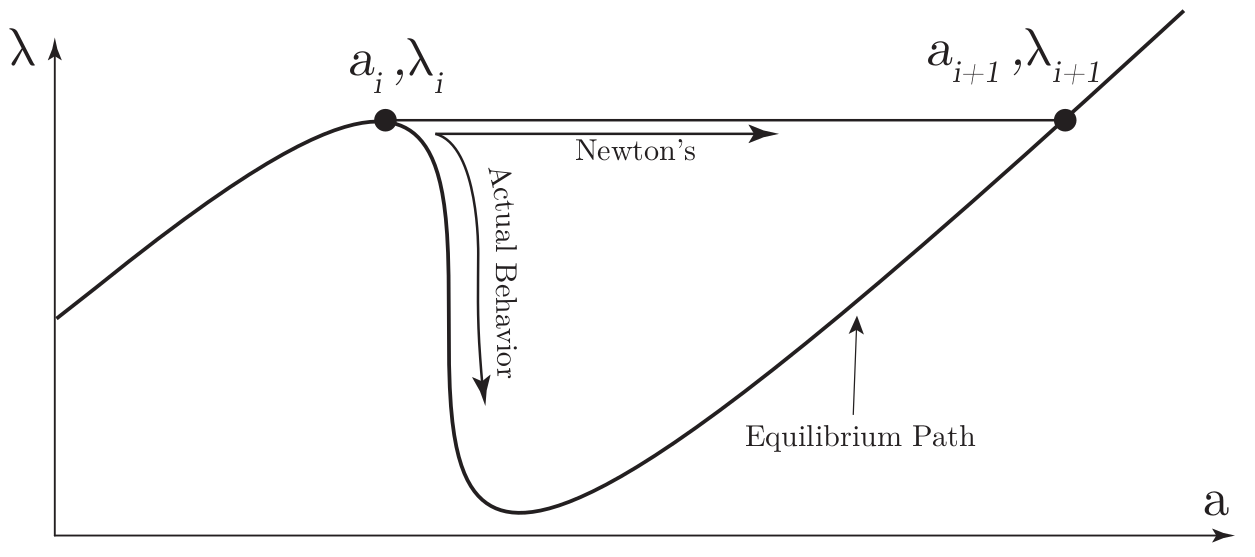
\includegraphics[width=0.6\textwidth]{newton_method_failure.png}
\caption{Failure of Newton's method to accurately capture the solution after a limit point is reached \cite{Vasios}}
\label{fig:2.17}
\end{figure}

\section{Finite deformations of torus membrane with free space}
For the geometry of our interest as observed in \Cref{fig:2.7.1}, we now study the elastic finite deformations of the torus magneto-elastic membrane with initial circular cross-section under a quasi-static inflating pressure load. The membrane is modelled as a non-linear elastic material employing the hyperelastic Neo-Hookean material model, cf. \Cref{eq:2.2}. The material parameter values for the magneto-elastic membrane were taken as $\mu = 3e^4$ Pa, $\nu = 0.4$. The surrounding free space (vacuum) through which the magnetic field $\mathbb{H}$ permeates is also modelled as a relatively less stiff elastic material, employing the same Neo-Hookean material model but with different material parameter values of $\mu = 3e^{-2}$ Pa and $\nu = 0.3$. Employing the total Lagrangian formulation, the inflating pressure load was applied on the undeformed/reference domain in uniformly increasing load steps as:

\begin{equation}
\mathbf{t}^p = \mathbf{P}\mathbf{N} = \left[ p_0 \mathbf{I} \right] \mathbf{N} = p_0 \mathbf{N},
\end{equation}

\noindent where $\mathbf{P}$ is the $1^{st}$ Piola-Kirchhoff stress, $p_0$ is the inflating pressure load (scalar) and $\mathbf{N}$ is the referential unit inward pointing normal vector for any point on the inner interface of the torus membrane. The inflating pressure load was taken as $p_0 = 1e^{3} \frac{\text{N}}{\text{m}^2}$. Homogeneous Dirichlet boundary condition was considered for the boundary of the free space domain.\par 

\begin{figure}[h]
\centering 
\begin{subfigure}[b]{0.6\textwidth}
\centering
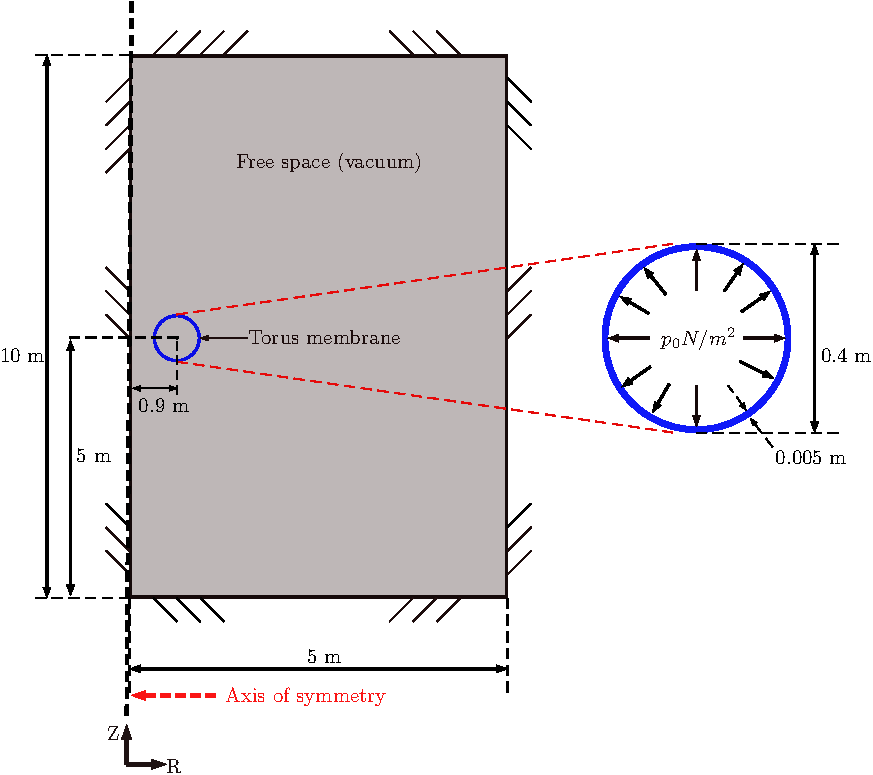
\includegraphics[width=0.9\textwidth]{torus_membrane_grid.pdf}
\caption{\scriptsize{Problem description}}
\label{fig:2.7.1}
\end{subfigure}
\begin{subfigure}[b]{0.39\textwidth}
\centering
\includegraphics[width=0.9\textwidth]{torus_grid_domain_decomp.png}
\caption{\scriptsize{Domain decomposition for 4 MPI processes}}
\label{fig:2.7.2}
\end{subfigure}
\caption{Magneto-elastic membrane under uniform inflating pressure load}
\label{fig:2.7}
\end{figure} 

The result of the above described uniformly inflating membrane problem is as observed in the \Cref{fig:2.9}. Due to the applied mechanical load, here quasi-static uniform inflating pressure load on inner interface of the membrane, large deformations are observed in the membrane and the surrounding elements of the free space. The deformations in the free space region far away from the torus membrane are small/negligible compared to the deformations in the elements belonging to the torus membrane. As observed in the displacement field of the deformed membrane (lower right image in \Cref{fig:2.9}), the deformations in the membrane are relatively large on the right half of the circular cross section when compared to the left half. This is due to the dependence of the deformation gradient $\mathbf{F}$ (component $F_{33}$) on the radial distance of the respective point on the membrane from the axis of symmetry, cf. \Cref{eq:2.26}. Thus, for any point on the torus membrane, with increasing radial distance the resulting displacements increase. \par  

\begin{figure}[h!]
\centering
\includegraphics[width=0.7\textwidth]{torus_disp_mue_1e6.pdf}
\caption{Deformations at full load}
\label{fig:2.9}
\end{figure}

For the considered free space parameters of $\mu = 3e^{-2}$ Pa and $\nu = 0.3$, one can observe that the free space material modelled with relatively less stiffness acts as a very complaint elastic material. This complaint elastic free space material allows for a free inflation of the membrane without any considerable reactive force/pressure load exerted by the free space material on the inflating membrane. The degree of deformations of the free space elements for increasing pressure load can be observed in \Cref{fig:2.10}. The torus membrane elements are ignored from the visualization and thus we observe a white circular section in the presented results.\par 

\begin{figure}[h!]
\centering 
\begin{subfigure}[b]{0.32\textwidth}
\centering
\includegraphics[width=0.95\textwidth]{vacuum_deformations_ls_0.png}
\caption{Load step 0 (no load)}
\label{fig:2.10.1}
\end{subfigure}
\begin{subfigure}[b]{0.32\textwidth}
\centering
\includegraphics[width=0.92\textwidth]{vacuum_deformations_half_load.png}
\caption{Load step 9 (Half load)}
\label{fig:2.10.2}
\end{subfigure}
\begin{subfigure}[b]{0.32\textwidth}
\centering
\includegraphics[width=0.93\textwidth]{vacuum_deformations_full_load.png}
\caption{Load step 19 (Full load)}
\label{fig:2.10.3}
\end{subfigure}
\caption{Free space (vacuum) deformations}
\label{fig:2.10}
\end{figure}

Element-wise volume averaged Cauchy stress $\bm{\sigma}$ components (radial component $\sigma_{rr}$ and theta component $\sigma_{\theta \theta}$) were also computed to have an understanding of the resulting engineering stress in the torus membrane. The element-wise volume averaged stress was computed as:
\begin{equation}
\left\langle \bm{\sigma} \right\rangle_e := \dfrac{\int\limits_{\Omega_{e}} \bm{\sigma} \mathrm{d}V_e}{\int\limits_{\Omega_{e}} \mathrm{d}V_e} = \dfrac{\sum\limits_{q} \bm{\sigma}(q) * J(q) * w(q)}{\sum\limits_{q} J(q) * w(q)}.
\end{equation}  
The resulting element averaged Cauchy stress components can be observed in \Cref{fig:2.11}. The dependence of the stress component $\sigma_{\theta \theta}$ on the radial distance of the point on the membrane from the axis of symmetry is clearly observed in \Cref{fig:2.11.2}. Thus, we observe a symmetry in the stress component field $\sigma_{\theta \theta}$ about the centre line cutting the membrane horizontally. Whereas a symmetry in the stress component field $\sigma_{rr}$ about the centre line cutting the membrane vertically can be observed in \Cref{fig:2.11.1}. \par 
 
\begin{figure}[ht!]
\centering 
\begin{subfigure}[b]{0.49\textwidth}
\centering
\includegraphics[width=0.9\textwidth]{membrane_avg_sigma_rr_mue_1e6.pdf}
\caption{$\sigma_{rr}$}
\label{fig:2.11.1}
\end{subfigure}
\begin{subfigure}[b]{0.49\textwidth}
\centering
\includegraphics[width=0.9\textwidth]{membrane_avg_sigma_tt_mue_1e6.pdf}
\caption{$\sigma_{\theta \theta}$}
\label{fig:2.11.2}
\end{subfigure}
\caption{Element averaged Cauchy stress components for torus membrane}
\label{fig:2.11}
\end{figure} 

\subsection{Parametric study of free space parameter $\mu$}
To model the free space material surrounding the torus membrane as a very compliant elastic we needed to select the elastic stiffness of the free space material such that there would be no reactive force by the free space material on the inflating torus membrane. For a selected less stiffer free space material one could then assume the torus membrane to inflate freely, adhering to the reality of the physics. Thus, a parametric study of the free space shear modulus $\mu$ was carried out for the finite strain axisymmetric torus elasticity problem. For the given inflating pressure load of $p_0 = 1e^{3} \frac{\text{N}}{\text{m}^2}$, torus membrane parameters $\mu = 3e^4$ Pa and $\nu = 0.4$, along with fixed value for the Poisson's ratio of the free space material as $\nu = 0.3$, the free space shear modulus $\mu$ was varied between $\mu_1 = 3e1$ Pa and $\mu_2 = 3e^{-2}$ Pa. \par 

As expected and observed in \Cref{fig:2.12}, with higher value of the free space shear modulus $\mu = 3e^{1}$ Pa the free space material acts more stiff and we observe the effect of this increased stiffness on the deformation of the torus membrane for the same applied pressure load. The resultant deformed state of the torus membrane in \Cref{fig:2.12.2} for the value of $\mu_1$, the stiffer free space material obstructs the free inflation of the membrane. Thus, we have relatively less deformed membrane when compared to the deformed state for $\mu_2$. \par 

\begin{figure}[h!]
\centering 
\begin{subfigure}[b]{0.49\textwidth}
\centering
\includegraphics[width=0.9\textwidth]{mue_study_1e3_vs_1e6_half_load.pdf}
\caption{Load step 9 (Half load)}
\label{fig:2.12.1}
\end{subfigure}
\begin{subfigure}[b]{0.49\textwidth}
\centering
\includegraphics[width=0.9\textwidth]{mue_study_1e3_vs_1e6_full_load.pdf}
\caption{Load step 19 (Full load)}
\label{fig:2.12.2}
\end{subfigure}
\caption{Deformations of torus membrane for different free space material parameter value $\mu$}
\label{fig:2.12}
\end{figure}

The resulting element averaged Cauchy stress components can be observed in \Cref{fig:2.13}. The developed stress due to larger deformations of the membrane for less stiffer ($\mu_2$) free space material is higher than the resulting stress for the more stiffer ($\mu_1$) free space material. \par 

\begin{figure}[h!]
\centering 
\begin{subfigure}[b]{0.49\textwidth}
\centering
\includegraphics[width=0.9\textwidth]{sigma_rr_1e3_vs_1e6_full_load.pdf}
\caption{$\sigma_{rr}$}
\label{fig:2.13.1}
\end{subfigure}
\begin{subfigure}[b]{0.49\textwidth}
\centering
\includegraphics[width=0.9\textwidth]{sigma_tt_1e3_vs_1e6_full_load.pdf}
\caption{$\sigma_{\theta \theta}$}
\label{fig:2.13.2}
\end{subfigure}
\caption{Element averaged Cauchy stress components of torus membrane for different free space material parameter value $\mu$}
\label{fig:2.13}
\end{figure}

For appropriate modelling of the membrane and free space with considered assumptions, it is necessary that we choose the material values for the free space such that we can closely approximate our free space material as being a compliant solid with negligible stiffness and thus exerting negligible loads on the inflating elastic torus membrane geometry of our interest. For values of $\mu < 3e^{-2}$ Pa, we observed negligible differences in the resulting deformed states and stress when compared to the results for the value of $\mu = 3e^{-2}$ Pa. Thus, a chosen value of $\mu \approx 3e^{-2}$ Pa can be considered as appropriate to model the free space. \par 

\section{Extensions planned for coupled problem}
The planned extensions for the next task are introducing the coupled problem and multi-physics employing a material model for the magneto-elastic material of our interest. The to be considered Neo-Hookean material model for the magneto-elastic material is given as
\begin{equation}
\Psi \equiv \dfrac{\mu}{2} [\mathbf{C} : \mathbf{I} - \mathbf{I} : \mathbf{I} - 2 \ln J] + \dfrac{\lambda}{2} (\ln J)^2 \textcolor{red}{- \dfrac{\mu_0 \mu_r}{2} \left[ J \ \mathbf{C}^{-1} : \mathbb{H} \otimes \mathbb{H} \right]}.
\end{equation}
The additional highlighted term takes into account the energy stored in the body due to applied external magnetic load $\mathbb{H}$ and the response of the coupled interaction between the displacement field and the magnetic field. The loads to be applied would be the uniformly distributed inflating pressure load on the inner interface of the torus membrane and the static magnetic field as mentioned in the results of previous Task 1. Furthermore, we would then consider the solution field to be comprised of two blocks, the scalar magnetic potential $\phi$ and the vector-valued displacement field $\mathbf{u}$. The corresponding linear algebra concepts for such a multi-physics problem are mentioned in further sections.

\subsection{Vector-valued problem} 
The solution in the elasticity problem discussed here is not just a single scalar function but has displacements $\mathbf{u} := \left\lbrace u_x, u_y, u_z \right\rbrace^T$ in each euclidean direction, thus we have a vector system which is a set of scalar functions and thus is also addressed as \textit{vector-valued solution}. When considering the coupled magneto-elastic problem, the resulting vector-valued solution has elements $\left\lbrace \phi, u_x, u_y, u_z \right\rbrace^T$. These elements of the vector-valued solution can be grouped into \textit{blocks}, where for the coupled magneto-elastic problem we have two blocks at each global degree of freedom in the finite element mesh, one block for the magnetic scalar potential function $\phi$ and the second block for the vector displacement function $\mathbf{u}$ with three individual components $u_x, u_y, u_z$ in 3D. This way one is able to access all the components/elements of the vector field such as displacement together without splitting them into their individual components. 

\subsection{Block linear algebra} 
Use of the block structure also proves advantageous in terms of linear algebra and solution methods. One can think of the global linear system of equation $\mathbf{A}\mathbf{x} = \mathbf{b}$ as
\begin{equation*}
\begin{bmatrix}
\mathbf{A}_{\phi\phi} & \mathbf{A}_{\phi \mathbf{u}} \\
\mathbf{A}_{\mathbf{u} \phi} & \mathbf{A}_{\mathbf{u}\mathbf{u}} 
\end{bmatrix}
\begin{bmatrix}
\phi \\
\mathbf{u}
\end{bmatrix} 
= 
\begin{bmatrix}
\mathbf{F_{\phi}} \\
\mathbf{F_{\mathbf{u}}}
\end{bmatrix},
\end{equation*}
where $\phi$ and $\mathbf{u}$ are the values of the scalar magnetic potential field and the displacement field. $\mathbf{A}_{\phi\phi}$ denotes the matrix contributions arising from the linearisation of the magnetic problem and $\mathbf{A}_{\mathbf{u}\mathbf{u}}$ describes the tangent matrix contribution from the elasticity problem. $\mathbf{A}_{\phi \mathbf{u}}$ and $\mathbf{A}_{\mathbf{u} \phi}$ are the coupled interaction contributions. One can solve the complete system considering as a single unit which can be convenient for the assembly of the matrix and right-hand-side vector for some class of problems. When employing the Gauss elimination rather than solving the problem monolithically, depending upon the properties of the (block) matrices for individual problem, one can then define individual preconditioners that best suite the operators present in the system of equations rather than defining a single preconditioner for the global matrix $\mathbf{A}$.

\subsection{Vector-valued Finite Elements} 
We shall consider here in all the discussions only \textit{primitive finite elements}. A finite element is said to be primitive if there is a unique relation from the shape function number to the vector component of the vector-valued element. This means for a primitive element we have exactly one non-zero component for each shape function of the vector-valued element. The Lagrangian elements that we shall employ are primitive elements. For the considered vector-valued coupled magneto-elastic problem we build the vector-valued finite element from simpler base elements using tensor product of the base elements. We take multiple simple elements (eg. scalar linear Lagrange elements $Q_1$) and connect them to have an element with more than one block. For the vector-valued displacement field in 2D, we can construct a vector-valued finite element using two $Q_1$ elements (each constituting to a single component $u_x$ and $u_y$) to form using a tensor product $Q_1 \times Q_1$ element with two components. This will form a single block in our coupled problem where the second block for the scalar magnetic potential will have only a single component such as a quadratic element $Q_2$. Thus, the vector-valued element we shall employ, for e.g., can be represented in block form as ($Q_1 \times Q_1, Q_2$) which will have in total $\text{dim}+1$ individual components in 2D as [$u_x, u_y, \phi$]. \newline 



\documentclass[11pt,a4paper,final]{article}
\usepackage[utf8]{inputenc}
\usepackage[T1]{fontenc}
\usepackage{amsmath}
\usepackage{amsfonts}
\usepackage{mathtools}
\usepackage{amssymb}
\usepackage{bm,bbm}
\usepackage[final]{graphicx}
\graphicspath{{./images/}}
\usepackage{caption}
\usepackage{subcaption}
\usepackage[usenames, dvipsnames]{color}
\usepackage[margin=1in]{geometry} % to adjust the page margins
%\pagenumbering{gobble} % To suppress page numbering 

\DeclarePairedDelimiterX{\norm}[1]{\lVert}{\rVert}{#1}
\newcommand{\seminorm}[1]{\left\lvert #1 \right\rvert}

\usepackage{breqn}
\usepackage{empheq}
\usepackage[most]{tcolorbox}

\usepackage{tikz,pgfplots}
\usetikzlibrary{spy}
\pgfplotsset{table/search path={./data}} %checks in data folder
\pgfplotsset{compat=newest}	%mention version to avoid warnings
\pgfplotsset{every axis/.append style={
                    label style={font=\small},
                    legend style={font=\small, draw=none, fill=none},
                    tick label style={font=\small}
                    }}

\usepackage{array}                            % better table support
\newcolumntype{C}[1]{>{\centering\arraybackslash}m{#1}}
\usepackage{multicol}                         % spanning columns
\usepackage{multirow}                         % spanning rows
\usepackage[ruled,vlined]{algorithm2e}
\usepackage{stmaryrd} % for jump in gradient symbol
\usepackage{siunitx}
\usepackage{textcomp} % for trademark and registered symbols
\usepackage[capitalise, noabbrev]{cleveref}
\usepackage[backend=biber,style=numeric,sorting=ynt]{biblatex}
\addbibresource{task2_ref.bib}

\begin{document}
\begin{center}
\textbf{\Large Master thesis: documentation of task 2.2}\\ \vspace{0.25cm}
\textbf{\large Vinayak Gholap}
\end{center}

\section{Tasks performed}
\begin{enumerate}
\item abc
\end{enumerate}

\section{Introduction}
Coupled magneto-elasticity problem. Multi-physics theory, arising difficulties, challenges in modelling. Summarising results and conclusions from task 1 and 2.1. 

\section{Constitutive material model for coupled problem}
The material response is characterised by a Helmholtz free energy density function. For the considered magneto-elastic material, in addition to the dependence on the deformation gradient $\mathbf{F}$ and the Jacobian $J$ (as already seen in quasi-static finite strain compressible elasticity, Task 2.1), the free energy density function now also depends on the referential magnetic vector field. The strain energy function (S.E.F.) is given as: 
\begin{equation}
\Psi = \Psi (J, \mathbf{F}, \mathbb{H}) = \Psi (J, \mathbf{C}, \mathbb{H}).
\label{eq:3.1}
\end{equation}
Using the symmetry argument from the definition of the right Cauchy-Green deformation tensor $\mathbf{C} := \mathbf{F}^T \cdot \mathbf{F}$, the dependence of $\mathbf{F}$ is simplified to a dependence on $\mathbf{C}$. The isotropic hyperelastic material response when $\mathbf{C}$ is used to describe the S.E.F. is given by the constitutive relation as
\begin{equation}
\mathbf{S} = 2 \dfrac{\partial \Psi (J, \mathbf{C}, \mathbb{H})}{\partial \mathbf{C}}.
\label{eq:3.2}
\end{equation}
The referential magnetic induction vector field $\mathbb{B}$ is modelled in terms of the referential magnetic vector field $\mathbb{H}$, taking $\mathbb{H}$ as the independent field
\begin{equation}
\mathbb{B} = \mathbb{B}(\mathbb{H}),
\label{eq:3.3}
\end{equation}
which is termed as the alternative formulation in \cite{dorfmann2004}. With $\mathbb{H}$ chosen as the independent field, its components can be chosen to satisfy the vector equation $\text{Curl} \mathbb{H} = \mathbf{0}$ and then the resulting $\mathbb{B}$ has to satisfy the scalar equation $\text{Div} \mathbb{B} = 0$. This alternative formulation does not put restrictions on the admissible class of constitutive laws (which arise if one were to proceed with $\mathbb{B}$ as the independent field) and also avoids the complexities of a vector-valued magnetic field from the finite element modelling aspects. The fundamental constitutive equation that relates the magnetic quantities $\mathbb{B}, \mathbb{H}$ and the magnetization vector $\mathbb{M}$ is given as \cite{dorfmann2004,dorfmann2005}
\begin{equation}
J^{-1} \mathbf{C} \cdot \mathbb{B} = \mu_0 \left[ \mathbb{H} + \mathbb{M} \right].
\label{eq:3.3.2}
\end{equation}
The magnetization vector field exists only in the solid magneto-elastic material and vanishes in the free space. $\mathbb{B}$ is given by another constitutive relation as \cite{dorfmann2004}: 
\begin{equation}
\mathbb{B} = -\dfrac{\partial \Psi (J, \mathbf{C}, \mathbb{H})}{\partial \mathbb{H}}.
\label{eq:3.4}
\end{equation}
The S.E.F corresponding to a compressible coupled magneto-elastic Neo-Hookean material is given as: 
\begin{align}
\Psi (J, \mathbf{C}, \mathbb{H}) &= \dfrac{\mu}{2} \left[ \mathbf{C} : \mathbf{I} - \mathbf{I} : \mathbf{I} -2 \ln J \right] + \dfrac{\lambda}{2} (\ln J)^2 \textcolor{red}{- \frac{\mu_0 \mu_r}{2} [J \mathbf{C}^{-1} : \mathbb{H} \otimes \mathbb{H}]}, \\
&= \Psi_0^{\text{elas}} (\mathbf{C}) + \mu_r M_0 (J, \mathbf{C}, \mathbb{H}), \\
& \text{with} \ M_0 (J, \mathbf{C}, \mathbb{H}) := -\frac{\mu_0}{2} [J \mathbf{C}^{-1} : \mathbb{H} \otimes \mathbb{H}],
\label{eq:3.5}
\end{align}
where $\mu$ and $\nu$ are the Lam\'e parameters, $\mu_0 = 4 \pi \times 10^{-7} \ \text{Hm}^{-1}$ is the free space (vacuum) magnetic permeability and $\mu_r$ is the relative magnetic permeability of the magneto-elastic material ($\mu_r = 1$ represents the free space material). The term highlighted in red takes into account the energy stored in the body due to applied external magnetic load $\mathbb{H}$ and the response of the coupled interaction between the displacement field and the magnetic field. The term $\Psi_0^{\text{elas}} (\mathbf{C})$ describes the purely elastic response of the material and the term $M_0 (J, \mathbf{C}, \mathbb{H})$ describes the total energy per unit volume stored in the magnetic fields in the free space \cite{dorfmann2004}. The constant $\mu_r > 1$ represents a magnetisable material such as the membrane. \par 

The second Piola-Kirchhoff stress $\mathbf{S}$ for the considered S.E.F. as stated in \Cref{eq:3.5} is derived below.
\begin{align*}
\mathbf{S} &= 2 \dfrac{\partial \Psi (J, \mathbf{C}, \mathbb{H})}{\partial \mathbf{C}} \\
&= 2 \left[ \dfrac{\mu}{2} \left\lbrace \dfrac{\partial [\mathbf{C} : \mathbf{I}]}{\partial \mathbf{C}} - 2 \dfrac{\partial \ln J}{\partial \mathbf{C}} \right\rbrace + \dfrac{\lambda}{2} \dfrac{\partial (\ln J)^2}{\partial \mathbf{C}} - \dfrac{\mu_0 \mu_r}{2} \dfrac{\partial [J \mathbf{C}^{-1} : \mathbb{H} \otimes \mathbb{H}]}{\partial \mathbf{C}} \right]
\end{align*}
Side calculation 1:
\begin{align*}
\dfrac{\partial [\mathbf{C} : \mathbf{I}]}{\partial \mathbf{C}} &= \mathbf{I} \\ 
\dfrac{\partial \ln J}{\partial \mathbf{C}} &= \dfrac{1}{J} \dfrac{\partial J}{\partial \mathbf{C}} \\
\dfrac{\partial (\ln J)^2}{\partial \mathbf{C}} &= 2 \ \ln J \ \dfrac{\partial \ln J}{\partial \mathbf{C}} \\
\dfrac{\partial J}{\partial \mathbf{C}} &= \dfrac{1}{2} J \mathbf{C}^{-1} \ \  \text{c.f. \cite[see][page 46 Equation (3.124)]{Wriggers2008}}
\end{align*}
\begin{align*}
\mathbf{S} &= \mu \mathbf{I} -  \mu \mathbf{C}^{-1} + \lambda \ln J \mathbf{C}^{-1} - \mu_0 \mu_r \dfrac{\partial [J \mathbf{C}^{-1} : \mathbb{H} \otimes \mathbb{H}]}{\partial \mathbf{C}}
\end{align*}
Side calculation 2: Note $\mathbf{C} := \mathbf{F}^T \cdot \mathbf{F} \ $ is symmetric $\implies \mathbf{C}^{-1}$ is also symmetric 
\begin{align*}
\dfrac{\partial [J \mathbf{C}^{-1} : \mathbb{H} \otimes \mathbb{H}]}{\partial \mathbf{C}} &= \dfrac{\partial [J C^{-1}_{IJ} H_I H_J]}{\partial C_{KL}} \ \mathbf{E}_K \otimes \mathbf{E}_L \\
&= C^{-1}_{IJ} \ H_I \ H_J \ \dfrac{\partial J}{\partial C_{KL}} \ \mathbf{E}_K \otimes \mathbf{E}_L + J \ H_I \ H_J \ \dfrac{\partial C^{-1}_{IJ}}{\partial C_{KL}} \ \mathbf{E}_K \otimes \mathbf{E}_L \\
&= C^{-1}_{IJ} \ H_I \ H_J \ \dfrac{J}{2} \ C^{-1}_{KL} \ \mathbf{E}_K \otimes \mathbf{E}_L + J \ H_I \ H_J \  \dfrac{\partial C^{-1}_{IJ}}{\partial C_{KL}} \ \mathbf{E}_K \otimes \mathbf{E}_L
\end{align*}
c.f. \cite[see][page 519]{Wriggers2008}: 
\begin{align*}
\dfrac{\partial C^{-1}_{IJ}}{\partial C_{KL}} = -\dfrac{1}{2} [C^{-1}_{IK} \ C^{-1}_{LJ} + C^{-1}_{IL} \ C^{-1}_{KJ}]
\end{align*}
\begin{align*}
\dfrac{\partial [J \mathbf{C}^{-1} : \mathbb{H} \otimes \mathbb{H}]}{\partial \mathbf{C}} &= \dfrac{J}{2} \ C^{-1}_{IJ} \ H_I \ H_J \ C^{-1}_{KL} \ \mathbf{E}_K \otimes \mathbf{E}_L + \dfrac{-J}{2} \left[ C^{-1}_{IK} \ C^{-1}_{LJ} \ H_I \ H_J + C^{-1}_{IL} \ C^{-1}_{KJ}  \ H_I \ H_J \right] \ \mathbf{E}_K \otimes \mathbf{E}_L \\
&= \dfrac{J}{2} \ C^{-1}_{IJ} \ H_I \ H_J \ C^{-1}_{KL} \ \mathbf{E}_K \otimes \mathbf{E}_L - \dfrac{J}{2} \left[ C^{-1}_{KI} \ H_I \ C^{-1}_{LJ} \ H_J + C^{-1}_{LI} \ H_I \ C^{-1}_{KJ} \ H_J \right] \ \mathbf{E}_K \otimes \mathbf{E}_L \\
&= \dfrac{J}{2} \ C^{-1}_{IJ} \ H_I \ H_J \ C^{-1}_{KL} \ \mathbf{E}_K \otimes \mathbf{E}_L - J [C^{-1}_{KI} \ H_I \ C^{-1}_{LJ} \ H_J]^{sym} \ \mathbf{E}_K \otimes \mathbf{E}_L \\
&= \dfrac{J}{2} [ \mathbf{C}^{-1} : \mathbb{H} \otimes \mathbb{H}] \mathbf{C}^{-1} - J [ (\mathbf{C}^{-1} \cdot \mathbb{H}) \otimes (\mathbf{C}^{-1} \cdot \mathbb{H})]^{sym}
\end{align*}
\begin{empheq}[box=\tcbhighmath]{equation}
\mathbf{S} = \mu \mathbf{I} - [\mu - \lambda \ln J] \mathbf{C}^{-1} - \dfrac{\mu_0 \mu_r}{2} \ J \ [ \mathbf{C}^{-1} : \mathbb{H} \otimes \mathbb{H}] \mathbf{C}^{-1} + \mu_0 \mu_r \ J \ [ (\mathbf{C}^{-1} \cdot \mathbb{H}) \otimes (\mathbf{C}^{-1} \cdot \mathbb{H})]^{sym}
\label{eq:3.6}
\end{empheq}

The referential magnetic induction vector field is given as:
\begin{align*}
\mathbb{B} &= - \dfrac{\partial \Psi (J, \mathbf{C}, \mathbb{H})}{\partial \mathbb{H}} \\
&= \dfrac{\mu_0 \mu_r}{2} \dfrac{\partial [J \ \mathbf{C}^{-1} : \mathbb{H} \otimes \mathbb{H}]}{\partial \mathbb{H}} \\
&= \dfrac{\mu_0 \mu_r}{2} \dfrac{\partial [J \ C^{-1}_{IJ} \ H_I \ H_J	]}{\partial H_K} \mathbf{E}_K \\
&= \dfrac{\mu_0 \mu_r}{2} \left[ J \ C^{-1}_{IJ} \dfrac{\partial H_I}{\partial H_K} \ H_J + J \ C^{-1}_{IJ} \ H_I \dfrac{\partial H_J}{\partial H_K} \right] \mathbf{E}_K \\
&= \dfrac{\mu_0 \mu_r}{2} \left[ J \ C^{-1}_{IJ} \ \delta_{IK} \ H_J + J \ C^{-1}_{IJ} \ H_I \ \delta_{JK} \right] \mathbf{E}_K \\
&= \dfrac{\mu_0 \mu_r}{2} \left[ J \ C^{-1}_{JI} \ \delta_{IK} \ H_J + J \ C^{-1}_{IJ} \ \delta_{JK} \ H_I \right] \mathbf{E}_K \\
&= \dfrac{\mu_0 \mu_r}{2} \left[ J \ C^{-1}_{JK} \ H_J + J \ C^{-1}_{IK} \ H_I \right] \mathbf{E}_K \\
&= \dfrac{\mu_0 \mu_r}{2} \left[ J \ C^{-1}_{KJ} \ H_J + J \ C^{-1}_{KI} \ H_I \right] \mathbf{E}_K
\end{align*}
\begin{empheq}[box=\tcbhighmath]{align}
\mathbb{B} = \mu_0 \mu_r \ J \ [\mathbf{C}^{-1} \cdot \mathbb{H}]
\label{eq:3.7}
\end{empheq}
The referential material elasticity tangent $\mathfrak{C}$ is defined as 
\begin{equation}
\mathfrak{C} := 2 \dfrac{\partial \mathbf{S}(J, \mathbf{C}, \mathbb{H})}{\partial \mathbf{C}} = 4 \dfrac{\partial^2 \Psi (J, \mathbf{C}, \mathbb{H})}{\partial \mathbb{C} \otimes \partial \mathbf{C}}.
\label{eq:3.8}
\end{equation} 
Using the result of \Cref{eq:3.6}, $\mathfrak{C}$ is derived as follows.
\begin{align*}
\mathfrak{C} &= 2 \dfrac{\partial \mathbf{S}}{\partial \mathbf{C}} \\
&= 2 \dfrac{\partial S_{KL}}{\partial C_{MN}} \ \mathbf{E}_K \otimes \mathbf{E}_L \otimes \mathbf{E}_M \otimes \mathbf{E}_N \\
\begin{split}
=\ & 2 \left\lbrace - \mathbf{C}^{-1} \otimes \dfrac{\partial [\mu - \lambda \ln J]}{\partial \mathbf{C}} - [\mu - \lambda \ln J] \dfrac{\partial \mathbf{C}^{-1}}{\partial \mathbf{C}} - \dfrac{\mu_0 \mu_r}{2} [\mathbf{C}^{-1} : \mathbb{H} \otimes \mathbb{H}] \ \mathbf{C}^{-1} \otimes \dfrac{\partial J}{\partial \mathbf{C}} \right\rbrace \\
&+ 2 \left\lbrace - \dfrac{\mu_0 \mu_r}{2} \ J \ \mathbf{C}^{-1} \otimes \dfrac{\partial [\mathbf{C}^{-1} : \mathbb{H} \otimes \mathbb{H}]}{\partial \mathbf{C}} - \dfrac{\mu_0 \mu_r}{2} \ J \ [\mathbf{C}^{-1} : \mathbb{H} \otimes \mathbb{H}] \dfrac{\partial \mathbf{C}^{-1}}{\partial \mathbf{C}} \right\rbrace \\
&+ 2 \left\lbrace \mu_0 \mu_r [ (\mathbf{C}^{-1} \cdot \mathbb{H}) \otimes (\mathbf{C}^{-1} \cdot \mathbb{H})]^{sym} \otimes \dfrac{\partial J}{\partial \mathbf{C}} + \mu_0 \mu_r \ J \ \dfrac{\partial [ (\mathbf{C}^{-1} \cdot \mathbb{H}) \otimes (\mathbf{C}^{-1} \cdot \mathbb{H})]^{sym}}{\partial \mathbf{C}} \right\rbrace
\end{split} \\
\begin{split}
=\ & 2 \left\lbrace C^{-1}_{KL} \ \dfrac{\lambda}{J} \dfrac{\partial J}{\partial C_{MN}} - [\mu - \lambda \ln J] \left\lbrace \dfrac{-1}{2} \left( C^{-1}_{KM} \ C^{-1}_{NL} + C^{-1}_{KN} \ C^{-1}_{ML} \right) \right\rbrace \right\rbrace \ \mathbf{E}_K \otimes \mathbf{E}_L \otimes \mathbf{E}_M \otimes \mathbf{E}_N\\
&+ 2 \left\lbrace - \dfrac{\mu_0 \mu_r}{2} \ [C^{-1}_{IJ} \ H_I \ H_J] C^{-1}_{KL} \dfrac{1}{2} \ J \ C^{-1}_{MN} - \dfrac{\mu_0 \mu_r}{2} J \ C^{-1}_{KL} \dfrac{\partial [C^{-1}_{IJ} \ H_I \ H_J]}{\partial C_{MN}} \right\rbrace \ \mathbf{E}_K \otimes \mathbf{E}_L \otimes \mathbf{E}_M \otimes \mathbf{E}_N \\
&+ 2 \left\lbrace - \dfrac{\mu_0 \mu_r}{2} \ J \ [C^{-1}_{IJ} \ H_I \ H_J] \left\lbrace \dfrac{-1}{2} (C^{-1}_{KM} \ C^{-1}_{NL} + C^{-1}_{KN} \ C^{-1}_{ML}) \right\rbrace \right\rbrace \ \mathbf{E}_K \otimes \mathbf{E}_L \otimes \mathbf{E}_M \otimes \mathbf{E}_N \\
&+ 2 \left\lbrace \mu_0 \mu_r [C^{-1}_{KI} \ H_I \ C^{-1}_{LJ} \ H_J]^{sym} \ \dfrac{1}{2} J \ C^{-1}_{MN} + \mu_0 \mu_r \ J \ \dfrac{\partial [C^{-1}_{KI} \ H_I \ C^{-1}_{LJ} \ H_J]^{sym}}{\partial C_{MN}} \right\rbrace \ \mathbf{E}_K \otimes \mathbf{E}_L \otimes \mathbf{E}_M \otimes \mathbf{E}_N
\end{split}\\
\begin{split}
=\ & \lambda \ C^{-1}_{KL} \ C^{-1}_{MN} + [\mu - \lambda \ln J] \left( C^{-1}_{KM} \ C^{-1}_{NL} + C^{-1}_{KN} \ C^{-1}_{ML} \right) - \dfrac{\mu_0 \mu_r}{2} \ J \ [C^{-1}_{IJ} \ H_I \ H_J] C^{-1}_{KL} \ C^{-1}_{MN}  \\
&- \mu_0 \mu_r J \ C^{-1}_{KL} \ \dfrac{\partial [C^{-1}_{IJ} \ H_I \ H_J]}{\partial C_{MN}} + \dfrac{\mu_0 \mu_r}{2} \ J \ [C^{-1}_{IJ} \ H_I \ H_J] (C^{-1}_{KM} \ C^{-1}_{NL} + C^{-1}_{KN} \ C^{-1}_{ML}) \\
&+ \mu_0 \mu_r \ J \ [C^{-1}_{KI} \ H_I \ C^{-1}_{LJ} \ H_J]^{sym} \ C^{-1}_{MN} + 2 \mu_0 \mu_r \ J \ \dfrac{\partial [C^{-1}_{KI} \ H_I \ C^{-1}_{LJ} \ H_J]^{sym}}{\partial C_{MN}} \ \mathbf{E}_K \otimes \mathbf{E}_L \otimes \mathbf{E}_M \otimes \mathbf{E}_N
\end{split}\\
\end{align*}
Side calculation 1:
\begin{align*}
\dfrac{\partial [C^{-1}_{IJ} \ H_I \ H_J]}{\partial C_{MN}} &= H_I \ H_J \ \dfrac{\partial C^{-1}_{IJ}}{\partial C_{MN}}\\
&= \dfrac{-1}{2} \ H_I \ H_J \ [C^{-1}_{IM} \ C^{-1}_{NJ} + C^{-1}_{IN} \ C^{-1}_{MJ}]\\
&= \dfrac{-1}{2} [C^{-1}_{MI} \ H_I \ C^{-1}_{NJ} \ H_J + C^{-1}_{NI} \ H_I \ C^{-1}_{MJ} \ H_J]\\
&= - [C^{-1}_{MI} \ H_I \ C^{-1}_{NJ} \ H_J]^{sym}\\
&= - [ (\mathbf{C}^{-1} \cdot \mathbb{H}) \otimes (\mathbf{C}^{-1} \cdot \mathbb{H}) ]^{sym}
\end{align*}
Side calculation 2:
\begin{align*}
\dfrac{\partial [C^{-1}_{KI} \ H_I \ C^{-1}_{LJ} \ H_J]^{sym}}{\partial C_{MN}} &= \dfrac{1}{2} \dfrac{\partial \left[ C^{-1}_{KI} \ H_I \ C^{-1}_{LJ} \ H_J + C^{-1}_{LI} \ H_I \ C^{-1}_{KJ} \ H_J \right] }{\partial C_{MN}}\\
\begin{split}
= & \ \dfrac{1}{2} \dfrac{\partial C^{-1}_{KI}}{\partial C_{MN}} \ H_I \ C^{-1}_{LJ} \ H_J + \dfrac{1}{2} C^{-1}_{KI} \ H_I \ \dfrac{\partial C^{-1}_{LJ}}{\partial C_{MN}} \ H_J \\
&+ \dfrac{1}{2} \dfrac{\partial C^{-1}_{LI}}{\partial C_{MN}} \ H_I \ C^{-1}_{KJ} \ H_J + \dfrac{1}{2} C^{-1}_{LI} \ H_I \ \dfrac{\partial C^{-1}_{KJ}}{\partial C_{MN}} \ H_J \\
\end{split}\\
\begin{split}
= & \ \dfrac{1}{2} \dfrac{-1}{2} \left[ C^{-1}_{KM} C^{-1}_{NI} + C^{-1}_{KN} C^{-1}_{MI} \right] \ H_I \ C^{-1}_{LJ} \ H_J \\
&+ \ \dfrac{1}{2} \dfrac{-1}{2} C^{-1}_{KI} \ H_I \left[ C^{-1}_{LM} C^{-1}_{NJ} + C^{-1}_{LN} C^{-1}_{MJ} \right] \ H_J \\
&+ \ \dfrac{1}{2} \dfrac{-1}{2} \left[ C^{-1}_{LM} C^{-1}_{NI} + C^{-1}_{LN} C^{-1}_{MI} \right] \ H_I \ C^{-1}_{KJ} \ H_J \\
&+ \ \dfrac{1}{2} \dfrac{-1}{2} C^{-1}_{LI} \ H_I \left[ C^{-1}_{KM} C^{-1}_{NJ} + C^{-1}_{KN} C^{-1}_{MJ} \right] \ H_J \\
\end{split}\\
\begin{split}
= &- \textcolor{blue}{\dfrac{1}{4} \left[ C^{-1}_{KM} \ C^{-1}_{NI} \ H_I \ C^{-1}_{LJ} \ H_J + C^{-1}_{KN} \ C^{-1}_{MI} \ H_I \ C^{-1}_{LJ} \ H_J \right]} \\
&- \textcolor{red}{\dfrac{1}{4} \left[ C^{-1}_{KI} \ H_I \ C^{-1}_{LM} \ C^{-1}_{NJ} \ H_J + C^{-1}_{KI} \ H_I \ C^{-1}_{LN} \ C^{-1}_{MJ} \ H_J \right]} \\
&- \textcolor{blue}{\dfrac{1}{4} \left[ C^{-1}_{LM} \ C^{-1}_{NI} \ H_I \ C^{-1}_{KJ} \ H_J + C^{-1}_{LN} \ C^{-1}_{MI} \ H_I \ C^{-1}_{KJ} \ H_J \right]} \\
&- \textcolor{red}{\dfrac{1}{4} \left[ C^{-1}_{LI} \ H_I \ C^{-1}_{KM} \ C^{-1}_{NJ} \ H_J + C^{-1}_{LI} \ H_I \ C^{-1}_{KN} \ C^{-1}_{MJ} \ H_J \right]}\\
\end{split}\\
&= -\textcolor{red}{\mathbb{X}} - \textcolor{blue}{\mathbb{Y}}
\end{align*}
The tensors with indices $\mathbf{E}_K \otimes \mathbf{E}_L \otimes \mathbf{E}_M \otimes \mathbf{E}_N$ are
\begin{align*}
\textcolor{red}{\mathbb{X}} &:= \dfrac{1}{4} \left[ C^{-1}_{KI} H_I C^{-1}_{LM} C^{-1}_{NJ} H_J + C^{-1}_{KI} H_I C^{-1}_{LN} C^{-1}_{MJ} H_J + C^{-1}_{LI} H_I C^{-1}_{KM} C^{-1}_{NJ} H_J + C^{-1}_{LI} H_I C^{-1}_{KN} C^{-1}_{MJ} H_J \right]\\
\textcolor{blue}{\mathbb{Y}} &:= \dfrac{1}{4} \left[ C^{-1}_{KM} C^{-1}_{NI} H_I C^{-1}_{LJ} H_J + C^{-1}_{KN} C^{-1}_{MI} H_I C^{-1}_{LJ} H_J + C^{-1}_{LM} C^{-1}_{NI} H_I C^{-1}_{KJ} H_J + C^{-1}_{LN} C^{-1}_{MI} H_I C^{-1}_{KJ} H_J \right]
\end{align*}
\noindent are both symmetric rank-4 tensors such that for given symmetric rank-2 tensors $\mathbf{M}, \mathbf{N}, \mathbf{P}, \mathbf{Q}$, we have:
\begin{align*}
\mathbf{N} &= \textcolor{red}{\mathbb{X}} : \mathbf{M}, \\
\mathbf{Q} &= \textcolor{blue}{\mathbb{Y}} : \mathbf{P}.
\end{align*}
\begin{align*}
\mathfrak{C} =  & \ \lambda \ \mathbf{C}^{-1} \otimes \mathbf{C}^{-1} -2 [\mu - \lambda \ln J] \ \dfrac{\partial \mathbf{C}^{-1}}{\partial \mathbf{C}} \\
&- \dfrac{\mu_0 \mu_r}{2} \ J \ [\mathbf{C}^{-1} : \mathbb{H} \otimes \mathbb{H}] (\mathbf{C}^{-1} \otimes \mathbf{C}^{-1}) + \mu_0 \mu_r \ J \ (\mathbf{C}^{-1} \otimes [ (\mathbf{C}^{-1} \cdot \mathbb{H}) \otimes (\mathbf{C}^{-1} \cdot \mathbb{H}) ]^{sym}) \\
&- \mu_0 \mu_r \ J \ [\mathbf{C}^{-1} : \mathbb{H} \otimes \mathbb{H}] \ \dfrac{\partial \mathbf{C}^{-1}}{\partial \mathbf{C}} + \mu_0 \mu_r \ J \ ([ (\mathbf{C}^{-1} \cdot \mathbb{H}) \otimes (\mathbf{C}^{-1} \cdot \mathbb{H}) ]^{sym} \otimes \mathbf{C}^{-1}) \\
&- 2 \mu_0 \mu_r \ J \ (\textcolor{red}{\mathbb{X}} + \textcolor{blue}{\mathbb{Y}})
\end{align*}
For given symmetric rank 2 tensors $\mathbf{A}$ and $\mathbf{B}$, we know: $\mathbf{A} \otimes \mathbf{B} = \mathbf{B} \otimes \mathbf{A}.$
\begin{empheq}[box=\tcbhighmath]{align}
\mathfrak{C} = & \ \lambda \ \mathbf{C}^{-1} \otimes \mathbf{C}^{-1} -2 [\mu - \lambda \ln J] \ \dfrac{\partial \mathbf{C}^{-1}}{\partial \mathbf{C}} \nonumber \\
&- \dfrac{\mu_0 \mu_r}{2} \ J \ [\mathbf{C}^{-1} : \mathbb{H} \otimes \mathbb{H}] (\mathbf{C}^{-1} \otimes \mathbf{C}^{-1}) - \mu_0 \mu_r \ J \ [\mathbf{C}^{-1} : \mathbb{H} \otimes \mathbb{H}] \ \dfrac{\partial \mathbf{C}^{-1}}{\partial \mathbf{C}} \nonumber \\
&+ 2 \mu_0 \mu_r \ J \ (\mathbf{C}^{-1} \cdot \mathbb{H}) \otimes (\mathbf{C}^{-1} \cdot \mathbb{H}) ]^{sym} \otimes \mathbf{C}^{-1}) - 2 \mu_0 \mu_r \ J \ (\textcolor{red}{\mathbb{X}} + \textcolor{blue}{\mathbb{Y}})
\label{eq:3.9}
\end{empheq}
The fourth-order referential material elasticity tensor possess both major and minor symmetries, i.e. $\mathfrak{C} = C_{KLMN} = C_{MNKL} = C_{KLNM} = C_{LKMN}$.

\section{Problem setup}
Geometry description. BC's and externally applied loads. Magnetic load and mechanical load. Load application setup. 

\section{Variational formulation}

The corresponding system of partial differential equations (the strong forms of the local balance equations) for each field, the scalar-valued magnetic potential field in Task 1 and the vector-valued displacement field for an axisymmetric solid in Task 2.1, were described in details. The required boundary conditions to formulate a boundary-value problem were also mentioned for both the individual field (decoupled) problems. We now consider the fully-coupled problem of the (axisymmetric) magneto-elastic membrane immersed in a free space. The strong form of the complete system for the coupled problem in the total Lagrangian formulation is as follows:
\begin{align}
\text{Kinematics}:& \ \mathbb{H}, \ \mathbf{F}, \ \mathbf{C} := \mathbf{F}^T \cdot \mathbf{F}, \ \mathbf{E} := \dfrac{1}{2} (\mathbf{C} - \mathbf{I}) \label{eq:3.22.1}\\
\text{Equilibrium}:& \ \text{Div} \mathbb{B} = 0 \label{eq:3.22.2}\\
& \ \text{Div}(\mathbf{F} \cdot \mathbf{S}) + \mathbf{b}^p = \mathbf{0} \label{eq:3.22.3}\\
\text{Constitutive equation}:& \ \mathbb{B} = -\dfrac{\partial \Psi (J, \mathbf{C}, \mathbb{H})}{\partial \mathbb{H}} \label{eq:3.22.4}\\
& \ \mathbf{S} = 2\dfrac{\partial \Psi (J, \mathbf{C}, \mathbb{H})}{\partial \mathbf{C}}.
\label{eq:3.22.5}
\end{align}
The boundary conditions to be enforced for each field are: 
\begin{align}
\mathbf{N} \cdot \llbracket \mathbb{B} \rrbracket = 0 \ \text{on} \ \partial \mathcal{S}_{0, \phi}, \label{eq:3.23.1}\\
\mathbf{u} = \mathbf{u}^p \ \text{on} \ \partial \mathcal{S}_{0, \mathbf{u}}, \label{eq:3.23.2}\\
\mathbf{F} \cdot \mathbf{S} \cdot \mathbf{N} = \mathbf{t}^p \ \text{on} \ \partial \mathcal{B}_{0, t}.
\label{eq:3.23.3}
\end{align}
\Cref{eq:3.23.1} at the bounding surface of the free space material enforces the normal component of the referential magnetic induction vector field to remain continuous on the specified boundary \cite{Pelteret2016}. This is a natural boundary condition in the unreformed configuration. \Cref{eq:3.23.2} is the homogeneous Dirichlet boundary condition for the displacement field. Here, the displacements on the free space boundary are constrained to zero. \Cref{eq:3.23.3} is the traction on the inner interface of the circular cross-section torus magneto-elastic membrane. From a mechanical perspective, this constitutes to a quasi-static inflating pressure load on the membrane and is analogues to an effect such as the air blown in a toy balloon to inflate the balloon. \newline \par 

\noindent \textbf{Principle of stationary potential energy:} \\
Based on the S.E.F. \Cref{eq:3.5}, to derive the weak form of the governing equations, we define the total potential energy function as
\begin{align}
\Pi &= \Pi_{int} + \Pi_{ext}, \\
\text{with} \ \Pi_{int} &= \int\limits_{\mathcal{D}_0} \Psi (J, \mathbf{C}, \mathbb{H}) \ \mathrm{d}V = \int\limits_{\mathcal{B}_0} \Psi_0^{\text{elas}} (\mathbf{C}) + \mu_r \int\limits_{\mathcal{B}_0} M_0 (J, \mathbf{C}, \mathbb{H}) + \int\limits_{\mathcal{S}_0} M_0 (J, \mathbf{C}, \mathbb{H}), \label{eq:3.24.1}\\
\text{and} \ \Pi_{ext} &= -\int\limits_{\mathcal{B}_0} \mathbf{u} \cdot \mathbf{b}^p \mathrm{d} V - \int\limits_{\partial \mathcal{B}_{0,t}} \mathbf{u} \cdot \mathbf{t}^p \mathrm{d}A -\int\limits_{\partial \mathcal{S}_{0,\mathbb{B}}} \phi \left[ \mathbb{B}_{\infty} \cdot \mathbf{N}_{\infty} \right] \mathrm{d}A.  
\label{eq:3.24.2}
\end{align}
The internal energy contribution \Cref{eq:3.24.1} is a sum of total potential energy per unit volume due to magneto-elastic material's deformation and magnetisation and the magnetic energy stored in the free space. The external energy contribution \Cref{eq:3.24.2} accounts for the referential mechanical body and traction forces respectively, and the last term describes the magnetic induction prescribed on the far-field boundary of the free space material. Due to the assumption that the magnetic field and magnetic induction are co-aligned, the last term in $\Pi_{ext}$ drops out. \par 

The stationary (saddle-)point $\min_{\mathbf{u}} \max_{\phi} \Pi \implies \delta \Pi$ describes the equilibrium solution to the coupled boundary value problem. The stationary point $\min_{\mathbf{u}} \max_{\phi} \Pi$ is that point at which all the directional derivatives of the total potential energy vanish. Using the G\^ateaux derivative we have
\begin{align}
\delta \Pi = D_{\delta \mathbf{u}} \Pi_{int} + D_{\delta \phi} \Pi_{int} + D_{\delta \mathbf{u}} \Pi_{ext} + D_{\delta \phi} \Pi_{ext} = 0.
\label{eq:3.25}
\end{align}
The components of the variation of the internal potential energy are given as \cite{Saxena2015}
\begin{align}
D_{\delta \mathbf{u}} \Pi_{int} &= \int\limits_{\mathcal{D}_0} \delta \mathbf{E} : \mathbf{S} \ \mathrm{d}V, \label{eq:3.26.1}\\
D_{\delta \phi} \Pi_{int} &= -\int\limits_{\mathcal{D}_0} \delta \mathbb{H} \cdot \mathbb{B} \ \mathrm{d}V,
\label{eq:3.26.2}
\end{align}
and that of the external potential energy are
\begin{align}
D_{\delta \mathbf{u}} \Pi_{ext} &= -\int\limits_{\mathcal{B}_0} \delta \mathbf{u} \cdot \mathbf{b}^p \mathrm{d}V - \int\limits_{\partial \mathcal{B}_{0,t}} \delta \mathbf{u} \cdot \mathbf{t}^p \mathrm{d}A, \label{eq:3.27.1}\\
D_{\delta \phi} \Pi_{ext} &= 0.
\label{eq:3.27.2}
\end{align}
The variations of the kinematic quantities are defined as 
\begin{align}
\delta \mathbf{F} &= \nabla_0 \delta \mathbf{u}, \\
\delta \mathbf{E} &= \left[ \mathbf{F}^T \cdot \delta \mathbf{F} \right]^{\text{sym}}, \\ 
\delta \mathbb{H} &= -\nabla_0 \delta \phi.
\label{eq:3.28}
\end{align}
The second Piola-Kirchhoff stress $\mathbf{S}$ in \Cref{eq:3.26.1} can further be split into two components, the total stress within the elastic body (membrane) and the Maxwell stress contribution from the free space (non-magnetisable) material respectively, as follows:
\begin{align}
\mathbf{S} &= \mathbf{S}^{\text{tot}} + \mathbf{S}^{\text{max}} =: 2 \dfrac{\partial \Psi (J, \mathbf{C}, \mathbb{H})}{\partial \mathbf{C}}, \\
\text{with} \ \mathbf{S}^{\text{tot}} &= 2 \dfrac{\partial \Psi_0^{\text{elas}} (\mathbf{C})}{\partial \mathbf{C}} + 2 \mu_r \dfrac{M_0 (J, \mathbf{C}, \mathbb{H})}{\partial \mathbf{C}}, \ \ (\text{note:} \ \mu_r > 1)\\
\text{and} \ \mathbf{S}^{\text{max}} &= 2 \dfrac{M_0 (J, \mathbf{C}, \mathbb{H})}{\partial \mathbf{C}}  \ \ (\text{note:} \ \mu_r = 1).
\end{align}
Similarly, the referential magnetic induction vector $\mathbb{B}$ in \Cref{eq:3.26.2} can be split into the induction within the elastic solid and the induction in the free space material as
\begin{align}
\mathbb{B} &= \mathbb{B}^{\text{tot}} + \mathbb{B}^{\text{max}} =: -\dfrac{\partial \Psi (J, \mathbf{C}, \mathbb{H})}{\partial \mathbb{H}}, \\
\text{with} \ \mathbb{B}^{\text{tot}} &= -\dfrac{\partial \Psi_0^{\text{elas}} (\mathbf{C})}{\partial \mathbb{H}} - \mu_r \dfrac{M_0 (J, \mathbf{C}, \mathbb{H})}{\partial \mathbb{H}}, \ \ (\text{note:} \ \mu_r > 1)\\
\text{and} \ \mathbb{B}^{\text{max}} &= -\dfrac{M_0 (J, \mathbf{C}, \mathbb{H})}{\partial \mathbb{H}}, \ \ (\text{note:} \ \mu_r = 1).
\end{align}
\Crefrange{eq:3.25}{eq:3.27.2} collectively represent the equivalent weak form of the equilibrium equations of our interest as mentioned in \Cref{eq:3.22.2,eq:3.22.3}. The continuity of the normal magnetic induction as given in \Cref{eq:3.23.1} at the material interfaces is also satisfied within this formulation. \par 

\noindent The variations in \Cref{eq:3.26.2,eq:3.27.1} belong to the following space
\begin{equation}
\delta \mathbf{u} \in H^1 (\overline{\mathcal{B}_0}), \ \ \delta \phi \in H^1 (\overline{\mathcal{B}_0}, \cup \mathcal{S}_0),
\end{equation}
with the constraints 
\begin{equation}
\delta \mathbf{u} = \mathbf{0} \ \text{on} \ \partial \mathcal{B}_{0,\mathbf{u}} \cup \left[ \overline{\mathcal{S}_0} \setminus \Gamma_{0, \mathcal{BS}} \right] \ \delta \phi = 0 \ \text{on} \ \partial \mathcal{B}_{0,\phi} \ \text{and} \ \partial \mathcal{S}_{0,\phi},
\end{equation}
where $\Gamma_{0, \mathcal{BS}} = \overline{\mathcal{S}_0} \cap \overline{\mathcal{B}_0}$ indicates the boundary of the magneto-elastic solid body exposed to the free space material. 


\section{FEM discretization}
Space discretization using finite elements. Final fem form using quadrature rule. 

\section{Implementation details}

\subsection{Saddle point system}
Theory on saddle point problems arising in coupled problems, compressible elasticity. Few properties of the block system in saddle point system and requirements to be satisfied to classify the linear system of equations as a saddle point system. \par 

A discretized system of linear equations valid for all the variations $\delta \mathbf{u}$ and $\delta \phi$ in the linearized variational formulation can be formed. At any Newton iteration $i$ and time step $t_n$ the algebraic equations are
\begin{equation}
\begin{bmatrix}
\mathbf{K}_{\phi \phi} & \mathbf{K}_{\phi \mathbf{u}} \\
\mathbf{K}_{\mathbf{u} \phi} & \mathbf{K}_{\mathbf{u} \mathbf{u}}
\end{bmatrix}
\begin{bmatrix}
\Delta \mathbf{d}_{\phi} \\
\Delta \mathbf{d}_{\mathbf{u}}
\end{bmatrix}
=
\begin{bmatrix}
-\mathbf{R}_{\phi} \\
-\mathbf{R}_{\mathbf{u}}
\end{bmatrix}
\implies \ \mathbf{K} \cdot \Delta \mathbf{d} = -\mathbf{R}.
\label{eq:3.10}
\end{equation}
Consider the scalar-valued magnetic potential solution block vector $\mathbf{d}_{\phi}$ be of size $p$ and the vector-valued displacement solution block vector $\mathbf{d}_{\mathbf{u}}$ for an axisymmetric formulation be of size $q$. Then the total number of unknowns, called as number of DoFs, will be $n_{dofs} = p + q$. For the case where the same order finite elements are employed for both the fields, for e.g., for a total number of support points $n_d$, for linear Lagrange finite element $(Q_1)$ used for the solution field $\phi$ with $p = n_d$ and bi-linear Lagrange finite elements $(Q_1 \times Q_1)$ for the solution field $\mathbf{u}$ with $q = 2 n_d$, then the total number of unknowns would be $n_{dofs} = 3 n_d$. By definition, a support point is a point $p_i$ such that for a shape function $N_j$ (finite element families based on the Lagrange interpolation) it holds $N_j (p_i) = \delta_{ij}$. The corresponding tangent matrix blocks will be of the following dimensions:
\begin{equation}
\mathbf{K}_{\phi \phi} \in \mathbb{R}^{p \times p}, \ \mathbf{K}_{\phi \mathbf{u}} \in \mathbb{R}^{p \times q}, \ \mathbf{K}_{\mathbf{u} \phi} \in \mathbb{R}^{q \times p}, \ \mathbf{K}_{\mathbf{u} \mathbf{u}} \in \mathbb{R}^{q \times q}.
\end{equation}
The increment in the solution $\Delta \mathbf{d} := \{ \Delta \mathbf{d}_{\phi}, \Delta \mathbf{d}_{\mathbf{u}} \}^T$ is then used to get the solution at the current unknown state $\mathbf{d}_{i+1}$ as
\begin{equation}
\mathbf{d}_{i+1} = \mathbf{d}_i + \Delta \mathbf{d}.
\end{equation} 
The system of equations in \Cref{eq:3.10} represents a saddle point system for the coupled multi-physics problem of our interest. Saddle point systems arise when a certain quantity such as the energy of a continuum body has to be minimized, subject to a set of linear constraints. The constraints typically represent some basic conservation law such as the balance law of linear momentum in our case of non-linear solid mechanics. Because saddle point systems can be derived as equilibrium conditions for a physical system, they are sometimes also referred to a \textit{equilibrium equations} \cite{Benzi2005}. We therefore briefly discuss the saddle point systems and also mention the necessary requirements to be satisfied for a linear system of equations to be classified as a saddle point system. \newline \par 
For a general linear system 
\begin{equation}
\begin{bmatrix}
\mathbf{A} & \mathbf{B} \\
\mathbf{C} & \mathbf{D}
\end{bmatrix}
\begin{bmatrix}
\mathbf{x} \\
\mathbf{y}
\end{bmatrix}
=
\begin{bmatrix}
\mathbf{f} \\
\mathbf{g}
\end{bmatrix}
\implies \mathbf{K} \cdot \mathbf{u} = \mathbf{r}
\label{eq:3.11}
\end{equation}
equivalent to \Cref{eq:3.10} to be classified as a (generalized) saddle point problem, the individual blocks $\mathbf{A}, \mathbf{B}, \mathbf{C}, \mathbf{D}$ of the tangent matrix $\mathbf{K}$ have to satisfy one or more of the following conditions \cite{Benzi2005}:
\begin{itemize}
\item[C1] $\mathbf{A}$ is symmetric: $\mathbf{A} = \mathbf{A}^T$
\item[C2] Symmetric part of $\mathbf{A}$, $\mathbf{A}^{sym} = \dfrac{1}{2} \left( \mathbf{A} + \mathbf{A}^T \right)$, is positive semidefinite
\item[C3] $\mathbf{B} = \mathbf{C}$
\item[C4] $\mathbf{D}$ is symmetric and positive semidefinite
\item[C5] $\mathbf{D} = \mathbf{0}$ (zero matrix)
\end{itemize}
When all the above conditions are satisfied, the tangent matrix $\mathbf{K}$ is symmetric positive semidefinite and we have a symmetric linear system of equations. Consider the following minimization problem:
\begin{equation}
J(\mathbf{u}) = \dfrac{1}{2} \left\langle \mathbf{K} \cdot \mathbf{u}, \mathbf{u} \right\rangle - \left\langle \mathbf{r}, \mathbf{u} \right\rangle,
\label{eq:3.12}
\end{equation}
subject to 
\begin{equation}
\mathbf{C} \cdot \mathbf{x} = \mathbf{g},
\label{eq:3.13}
\end{equation}
with $\left\langle \cdot, \cdot \right\rangle$ denoting the standard inner product in $\mathbb{R}^{p+q}$.
Note that
\begin{equation}
\nabla J(\mathbf{u}) = \mathbf{K} \cdot \mathbf{u} - \mathbf{r}.
\end{equation}
Any solution $(\mathbf{x}_{\ast}, \mathbf{y}_{\ast})^T$ of the general case (satisfying all of the conditions C1-C5), is a saddle point of the Lagrangian defined as
\begin{equation}
\mathcal{L}(\mathbf{x}, \mathbf{y}) = \dfrac{1}{2} \left\langle \mathbf{K} \cdot \mathbf{u}, \mathbf{u} \right\rangle - \left\langle \mathbf{r}, \mathbf{u} \right\rangle + (\mathbf{C} \cdot \mathbf{x} - \mathbf{g})^T \cdot \mathbf{y}.
\label{eq:3.14}
\end{equation}
The saddle point $(\mathbf{x}_{\ast}, \mathbf{y}_{\ast})^T \in \mathbb{R}^{p+q}$ satisfies
\begin{equation}
\mathcal{L}(\mathbf{x}_{\ast}, \mathbf{y}) \leq \mathcal{L}(\mathbf{x}_{\ast}, \mathbf{y}_{\ast}) \leq \mathcal{L}(\mathbf{x}, \mathbf{y}_{\ast}) \ \forall \mathbf{x} \in \mathbb{R}^p \ \& \ \forall \mathbf{y} \in \mathbb{R}^q, 
\label{eq:3.15.1}
\end{equation}
or equivalently, 
\begin{equation}
\min_{\mathbf{x}} \max_{\mathbf{y}} \mathcal{L}(\mathbf{x}, \mathbf{y}) = \mathcal{L}(\mathbf{x}_{\ast}, \mathbf{y}_{\ast}) = \max_{\mathbf{x}} \min_{\mathbf{y}} \mathcal{L}(\mathbf{x}, \mathbf{y}).
\label{eq:3.15.2}
\end{equation}

\begin{figure}[h]
\centering
\includegraphics[width=0.6\textwidth]{saddle_point_problem.png}
\caption{Saddle point over a 3D surface \cite{Buduma_book}}
\label{fig:3.1}
\end{figure}

A better understanding of \Cref{eq:3.15.1,eq:3.15.2} can be observed in \Cref{fig:3.1}. Depending upon how one cuts the surface moving along the direction A to B or from C to D (orthogonal direction to A to B), the critical point looks like a local minima or a local maxima, but in reality it is neither. It is a saddle point. \par 

\Cref{eq:3.10} for the coupled multi-physics problem of magneto-elastic membrane in free space is a special case of the (generalized) saddle point system. Here, the conditions C1-C4 are satisfied, but not C5 which arises in the discretization of equations describing slightly compressible solids \cite{Benzi2005}.

\subsection{Numerical solution of saddle point systems}
Iterative method using preconditioners: Schur complement method. Algorithm. Use of preconditioners (AMG theory?). Use of linear operator data structure from deal.ii. \par 

Explain the LSAE for our coupled problem. The properties of each block of the matrix. Choice of the block to proceed with schur complement of that block of matrix (why phi phi block?). Precomputations performed to transform the corresponding block from neg def to pos def (for solution by use of iterative method such as CG). \par 

Direct solution method: Monolithic approach using UMFPACK. Assembly in serial block solution and rhs vectors. 

To solve the linear system of equations \Cref{eq:3.10}, one of the following approach can be taken:
\begin{itemize}
\item Direct solver solving the complete system monolithically.
\item Global iterative solver with a global preconditioner constructed for the tangent matrix $\mathbf{K}$.
\item Sequentially solve for each unknown field $\phi$ and $\mathbf{u}$ exploiting the tangent matrix's block structure.
\end{itemize}
Below we explain the direct solver and the iterative solution method exploiting the block structure that were implemented. Before we discuss the details of the solution methods, it is important to highlight the properties of each block in the tangent matrix $\mathbf{K}$. This will also explain the motive for the choice of block to proceed with iterative solution method detailed in the further section.\par 

As observed in the finite element discretized form for the coupled problem, the block for purely magnetic scalar potential contribution $\mathbf{K}_{\phi \phi} = - \int\limits_{\mathcal{D}_0} \nabla_0 N^I \cdot \mathbf{D} \cdot \nabla_0 N^J$ results in a symmetric negative-definite matrix of size $p \times p$. The block for purely non-linear elastic contribution $\mathbf{K}_{\mathbf{u} \mathbf{u}} = \int\limits_{\mathcal{D}_0} \left[ \left[ \nabla_0^T \mathbf{N}^I \cdot \nabla_0 \mathbf{N}^J \right] : \mathbf{S} + \left[ \mathbf{F}^T \cdot \nabla_0 \mathbf{N}^I \right] : \mathfrak{C} : \left[ \mathbf{F}^T \cdot \nabla_0 \mathbf{N}^J \right] \right]$ represents a symmetric positive-definite matrix of size $q \times q$. For the considered axisymmetric problem, we know that for any given total number of support points $n_d$, $p < q$ given that we solve for a single scalar-valued magnetic potential $\phi$ and a vector-valued displacement $(u_r, u_z)^T$. Thus, the size of block $\mathbf{K}_{\phi \phi}$ is always less than the block $\mathbf{K}_{\mathbf{u} \mathbf{u}}$ (unless we solve for a 1D problem). The blocks resulting from the coupling between the two fields, namely $\mathbf{K}_{\phi \mathbf{u}}$ and $\mathbf{K}_{\mathbf{u} \phi}$ are symmetric negative-definite matrices with sizes $p \times q$ and $q \times p$, respectively and are transposes of each other. Thus, one can assemble one block and store the other as the transpose of the assembled block to save computations. Due to the sparsity arising in each individual block, the structure of the tangent matrix $\mathbf{K}$ is an unsymmetric sparse banded block matrix.\par 

\subsubsection{Direct solver}
This category of solvers is also known as `\textit{coupled}' or `all at once' methods. Coupled solvers deal with the system such as \Cref{eq:3.10} as a whole, computing both the fields $\phi$ and $\mathbf{u}$ simultaneously and without making any explicit use of reduced systems. In most cases, due to the ease of implementation, the direct solver is employed. One doesn't have to care about the properties of the tangent matrix $\mathbf{K}$ and also about the properties of individual blocks. \par 

We use a sparse direct solver called UMFPACK \cite{davis2004algorithm}, which is part of the SuiteSparse library \cite{davis2015suitesparse}. Interface to this solver is provided in the \texttt{deal.II} \cite{Alzetta2018} library in the form of the class \textbf{SparseDirectUMFPACK}. UMFPACK is a set of routines for solving unsymmetric sparse linear systems of the form $\mathbf{A} \cdot \mathbf{x} = \mathbf{b}$. It employs the unsymmetric multifrontal method and direct sparse LU factorization. It is heavily used as a built-in routine in MATLAB\textsuperscript{\tiny\sffamily\textregistered} and appears as lu and $\mathbf{x} = \mathbf{A} \setminus \mathbf{b}$ (back slash operator). It is important to note that this solver is a serial solver and therefore one cannot employ parallel (MPI) data structures for the vectors and reap the benefits of distributed memory parallelism for a large system of equations. Thus, solution time for a large system using such a serial direct solver would be high compared to a parallelized iterative solver in most cases. But for our problem of interest, in axisymmetric formulation it was observed that the computation time for the total solution was comparable to that of a parallelized iterative solver mentioned in the next section.

\subsubsection{Segregated iterative solver using Schur complement reduction}
The other category of solvers is the so called segregated solver which computes both the unknown fields $\phi$ and $\mathbf{u}$ separately. This approach involves the solution of two linear systems of size smaller than $p+q$ which are termed as \textit{reduced systems}. One reduced system is formed for the field $\phi$ and the other reduced system for the field $\mathbf{u}$. Depending upon the number of unknown fields, for example, in cases of a Lagrange multiplier, a separate reduced system for that unknown field is also formed and solved. Here, we shall look at one of the representatives of such a segregated approach known as the Schur complement reduction which we implemented for the solution of the fully-coupled magneto-elastic problem of our interest. \par 

The Schur complement reduction is based on the block LU factorization of the sparse block tangent matrix $\mathbf{K}$. Consider the saddle point system of our interest  from \Cref{eq:3.10}:
\begin{equation}
\mathbf{K}_{\phi \phi} \cdot \Delta \mathbf{d}_{\phi} + \mathbf{K}_{\phi \mathbf{u}} \cdot \Delta \mathbf{d}_{\mathbf{u}} = -\mathbf{R}_{\phi}, \ \ \mathbf{K}_{\mathbf{u} \phi} \cdot \Delta \mathbf{d}_{\phi} + \mathbf{K}_{\mathbf{u} \mathbf{u}} \cdot \Delta \mathbf{d}_{\mathbf{u}} = -\mathbf{R}_{\mathbf{u}}. 
\label{eq:3.16}
\end{equation}
If the block $\mathbf{K}_{\phi \phi}$ is square and non-singular (invertible), which in our case is true, the saddle point matrix $\mathbf{K}$ admits the following block triangular factorization:
\begin{equation}
\mathbf{K} = 
\begin{bmatrix}
\mathbf{K}_{\phi \phi} & \mathbf{K}_{\phi \mathbf{u}} \\
\mathbf{K}_{\mathbf{u} \phi} & \mathbf{K}_{\mathbf{u} \mathbf{u}}
\end{bmatrix} 
= 
\begin{bmatrix}
\mathbf{I} & \mathbf{0} \\
\mathbf{K}_{\mathbf{u} \phi} \mathbf{K}_{\phi \phi}^{-1} & \mathbf{I}
\end{bmatrix}
\begin{bmatrix}
\mathbf{K}_{\phi \phi} & \mathbf{0} \\
\mathbf{0} & \mathbf{S}
\end{bmatrix}
\begin{bmatrix}
\mathbf{I} & \mathbf{K}_{\phi \phi}^{-1} \mathbf{K}_{\phi \mathbf{u}}^T \\
\mathbf{0} & \mathbf{I}
\end{bmatrix},
\label{eq:3.17}
\end{equation} 
where $\mathbf{I}$  and $\mathbf{0}$ are the unit identity matrix and null matrix of appropriate size, respectively. The matrix $\mathbf{S}$ is the Schur complement of block $\mathbf{K}_{\phi \phi}$ in $\mathbf{K}$ and is defined as:
\begin{equation}
\mathbf{S} = \mathbf{K}_{\mathbf{u} \mathbf{u}} - \mathbf{K}_{\mathbf{u} \phi} \mathbf{K}_{\phi \phi}^{-1} \mathbf{K}_{\phi \mathbf{u}} \equiv \mathbf{D} - \mathbf{C} \mathbf{A}^{-1} \mathbf{B} \ \text{from \Cref{eq:3.11}}.
\label{eq:3.18}
\end{equation}
With the magnetic potential stiffness block $\mathbf{K}_{\phi \phi}$ and the total stiffness matrix $\mathbf{K}$ being square and invertible, by the block triangular factorization in \Cref{eq:3.17} the Schur complement $\mathbf{S}$ is also invertible. Pre-multiplying both the sides of the first equation in \Cref{eq:3.16} by $\mathbf{K}_{\mathbf{u} \phi} \mathbf{K}_{\phi \phi}^{-1}$, we obtain
\begin{equation}
\mathbf{K}_{\mathbf{u} \phi} \cdot \Delta \mathbf{d}_{\phi} +  \mathbf{K}_{\mathbf{u} \phi} \mathbf{K}_{\phi \phi}^{-1} \mathbf{K}_{\phi \mathbf{u}} \cdot \Delta \mathbf{d}_{\mathbf{u}} = -\mathbf{K}_{\mathbf{u} \phi} \mathbf{K}_{\phi \phi}^{-1} \cdot \mathbf{R}_{\phi}.
\end{equation}
Using $\mathbf{K}_{\mathbf{u} \phi} \cdot \Delta \mathbf{d}_{\phi} = -\mathbf{R}_{\mathbf{u}} - \mathbf{K}_{\mathbf{u} \mathbf{u}} \cdot \Delta \mathbf{d}_{\mathbf{u}}$ from the second equation in \Cref{eq:3.16}, after rearranging we see
\begin{equation}
\left( \mathbf{K}_{\mathbf{u} \mathbf{u}} - \mathbf{K}_{\mathbf{u} \phi} \mathbf{K}_{\phi \phi}^{-1} \mathbf{K}_{\phi \mathbf{u}} \right) \cdot \Delta \mathbf{d}_{\mathbf{u}} = \mathbf{K}_{\mathbf{u} \phi} \mathbf{K}_{\phi \phi}^{-1} \cdot \mathbf{R}_{\phi} - \mathbf{R}_{\mathbf{u}} \implies \mathbf{S} \cdot \Delta \mathbf{d}_{\mathbf{u}} = \mathbf{R}_{\mathbf{u}}^',
\label{eq:3.19}
\end{equation}
with the modified right-hand side vector $\mathbf{R}_{\mathbf{u}}^' := \mathbf{K}_{\mathbf{u} \phi} \mathbf{K}_{\phi \phi}^{-1} \cdot \mathbf{R}_{\phi} - \mathbf{R}_{\mathbf{u}}$ arising from the condensation step.
In terms of the general representation as in \Cref{eq:3.11}, we arrive at
\begin{equation}
\left( \mathbf{D} - \mathbf{C} \mathbf{A}^{-1} \mathbf{B} \right) \cdot \mathbf{y} = \mathbf{g} - \mathbf{C} \mathbf{A}^{-1} \mathbf{f} \implies \mathbf{S} \cdot \mathbf{y} = \mathbf{g}^'.
\label{eq:3.20} 
\end{equation}
\Cref{eq:3.19,eq:3.20} represent a reduced system of order $q$ for the solution update in displacement field $\Delta \mathbf{d}_{\mathbf{u}}$. It is important to note that unless $-\mathbf{R}_{\phi} \equiv \mathbf{f} = \mathbf{0}$, pre-processing the condensed right-hand side vector $\mathbf{R}_{\mathbf{u}}^' \equiv \mathbf{g}^'$ requires solving another linear system of equation of the form $\mathbf{A} \cdot \mathbf{v} = \mathbf{f}$. Once the solution (or an approximation) $\Delta \mathbf{d}_{\mathbf{u}}$ of the reduced system \Cref{eq:3.19} is computed, we then post-process the solution update for the other field $\Delta \mathbf{d}_{\phi}$ using the solution from the first update $\Delta \mathbf{d}_{\mathbf{u}}$ as
\begin{equation}
\mathbf{K}_{\phi \phi} \cdot \Delta \mathbf{d}_{\phi} = -\mathbf{R}_{\phi} - \mathbf{K}_{\phi \mathbf{u}} \cdot \Delta \mathbf{d}_{\mathbf{u}}.
\label{eq:3.21}
\end{equation}
\Cref{eq:3.21} represents the other reduced system of size $p$ that needs to be solved for the magnetic potential solution update. \Cref{alg:3.1} highlights the algorithmic steps needed to solve any saddle point system using the segregated iterative solver. The algorithm is explained for the fully-coupled magneto-elastic problem of our interest, solving for the displacement field first and then for the magnetic potential, but can be applied for any general saddle point system such as \Cref{eq:3.11}.

\begin{algorithm}[h]
\begin{enumerate}
\item Define the inverse $\mathbf{K}_{\phi \phi}^{-1}$ using a solver with preconditioner.
\item Define the Schur complement $\mathbf{S} = \mathbf{K}_{\mathbf{u} \mathbf{u}} - \mathbf{K}_{\mathbf{u} \phi} \mathbf{K}_{\phi \phi}^{-1} \mathbf{K}_{\phi \mathbf{u}}$.
\item Define the inverse of the Schur complement $\mathbf{S}^{-1}$ using another solver with a preconditioner to compute the approximate inverse operation of $\mathbf{S}$. 
\item Perform the pre-processing step to condense the right-hand side vector $\mathbf{R}_{\mathbf{u}}^' := \mathbf{K}_{\mathbf{u} \phi} \mathbf{K}_{\phi \phi}^{-1} \cdot \mathbf{R}_{\phi} - \mathbf{R}_{\mathbf{u}}$.
\item Solve for the solution update $\Delta \mathbf{d}_{\mathbf{u}}$: $\Delta \mathbf{d}_{\mathbf{u}} = \mathbf{S}^{-1} \cdot \mathbf{R}_{\mathbf{u}}^'$.
\item Post-process the solution for the other field: $\Delta \mathbf{d}_{\phi} = \mathbf{K}_{\phi \phi}^{-1} \left( -\mathbf{R}_{\phi} - \mathbf{K}_{\phi \mathbf{u}} \cdot \Delta \mathbf{d}_{\mathbf{u}} \right)$. 
\end{enumerate}
\caption{Schur complement reduction}
\label{alg:3.1}
\end{algorithm}

\begin{large}
\noindent \textbf{Choice of the block to compute the Schur complement of $\mathbf{K}$:}\\
\end{large}
\indent The choice of the block $\mathbf{K}_{\phi \phi}$  of size $p \times p$ to proceed with the Schur complement of $\mathbf{K}$ is due to the small size of the block compared to the other diagonal block $\mathbf{K}_{\mathbf{u} \mathbf{u}}$ of size $q \times q$, with $p < q$ as mentioned in the previous section. The motive behind the choice of the block of small size is the need to compute the inverse of the chosen block in computing the Schur complement $\mathbf{S}$ as observed in \Cref{eq:3.18}. Computational cost of computing the inverse of a matrix of size $q \times q$ exceeds that of the cost for a matrix of size $p \times p$. One also needs to take into account the lower bandwidth of the scalar magnetic potential stiffness matrix block compared to that of the displacement stiffness matrix block \cite{Pelteret2016}. \newline \par 

Typically this inversion of the chosen block matrix is performed by using a robust Krylov subspace iterative solver such as the Conjugate Gradient method with some form of preconditioning. The CG method works on only symmetric positive-definite matrices \cite{EdwinK.P.Chong2013}. Whereas the block $\mathbf{K}_{\phi \phi}$ and $\mathbf{K}_{\phi \mathbf{u}}$ of the first equation in \Cref{eq:3.16} are symmetric negative-definite matrices. In order to compute the inverse $\mathbf{K}_{\phi \phi}^{-1}$ using the CG iterative solver we need to transform the matrix $\mathbf{K}_{\phi \phi}$ to a positive-definite matrix. We do this by multiplying the first equation in \Cref{eq:3.16} by a factor of -1. This leads to a system of equations as
\begin{equation}
-\mathbf{K}_{\phi \phi} \cdot \Delta \mathbf{d}_{\phi} - \mathbf{K}_{\phi \mathbf{u}} \cdot \Delta \mathbf{d}_{\mathbf{u}} = \mathbf{R}_{\phi},
\end{equation}
with symmetric positive-definite matrix blocks. The matrix block $\mathbf{K}_{\phi \phi}$ is preconditioned to reduce the condition number and thus have a good convergence rate within the iterative solver computing an approximation to the inverse $\mathbf{K}_{\phi \phi}^{-1}$. We have employed the Trilinos \cite{heroux2005overview} linear algebra suite for the parallel and efficient data structures of vectors, matrices, preconditioners and solvers. Jacobi, SSOR and the Algebraic Multigrid (AMG) \cite{gee2006ml} preconditioners were used from the Trilinos suite. Depending on a user input parameter one of the three would be used. To compute the inverse $\mathbf{K}_{\phi \phi}^{-1}$ a reduced-iteration CG solver was employed. The linear transformations such as the scaling of matrix with a factor of -1, forming the inverse operator $\mathbf{K}_{\phi \phi}^{-1}$ and the Schur complement $\mathbf{S}$ was carried out using the class \textbf{LinearOperator} from the \texttt{deal.II} library. Lazy evaluation of linear transformations and expressions using vectors and matrices is performed by this class. The lazy evaluation of an expression helps in avoiding any intermediate storage of temporary objects. The class stores the sequence of operations that need to be performed on the vector/matrix object and executes them only when the value of the object is required. The class \textbf{LinearOperator} provides several member functions that aid the user implementing a Schur complement reduction solver. The member function \textbf{linear\_operator()} was used on each block of the tangent matrix $\mathbf{K}$ to transform the underlying Trilinos sparse matrix to a \textbf{LinearOperator} data structure. The function \textbf{inverse\_operator()}, which takes the matrix of which inverse is to be computed, the iterative linear solver and the preconditioner for the matrix as arguments, was employed to form the inverse operator $\mathbf{K}_{\phi \phi}^{-1}$. The Schur complement was defined using the member function \textbf{schur\_complement()} which takes the four matrix blocks as arguments required to define the Schur complement $\mathbf{S} := \mathbf{D} - \mathbf{C} \mathbf{A}^{-1} \mathbf{B}$. \par 

Another reduced-iteration CG solver was used with one of the three precondtioner to define the inverse operator for the Schur complement $\mathbf{S}^{-1}$. To pre-process the condensed right-hand side vector as mentioned in \Cref{alg:3.1}, the member function \textbf{condense\_schur_rhs()} of the class \textbf{LinearOperator} was employed. To post-process the solution update for the second field the member function \textbf{postprocess\_schur_solution()} was employed. Thus, in total two different iterative solvers with respective preconditioners were implemented within the Schur complement reduction method. An inner solver to compute $\mathbf{K}_{\phi \phi}^{-1}$ and an outer solver to compute $\mathbf{S}^{-1}$.

\section{Test case and Results}
\subsection{Unit test problem}

\subsection{Torus problem}
With mechanical load applied first, followed by magnetic load. Results. Conclusion. \par 

With magnetic load applied first, followed by mechanical load (to observe mechanically induced instabilities in the membrane). Results and conclusions.


\newpage
\printbibliography
\end{document}

\appendix
\chapter{Appendix}
\textbf{1. Sample}



\manualmark
\markleft{List of Acronyms}
\markright{List of Acronyms}
%\printglossary
\cleardoublepage

\markleft{Index}
\markright{Index}
\printindex

\automark[chapter]{section}
%\bibliographystyle{plain}
\printbibliography[heading=bibintoc]


\end{document}
